\documentclass[11pt,letterpaper]{article}
\usepackage[T1]{fontenc}
\usepackage[utf8]{inputenc}
\usepackage{lmodern,microtype}
\usepackage[margin=1.02in,top=.96in,bottom=1in,headheight=15pt]{geometry}
\usepackage{amsmath,amssymb,amsthm,mathtools,booktabs,longtable,tabularx,array,enumitem}
\usepackage{graphicx,xcolor,tikz,fancyhdr,needspace,xurl,multicol}
\definecolor{ink}{HTML}{17364A}
\definecolor{accent}{HTML}{11655D}
\definecolor{lighttone}{HTML}{E6F1EE}
\usepackage[colorlinks=true,linkcolor=ink,urlcolor=accent,citecolor=accent]{hyperref}
\usepackage{bookmark}
\hypersetup{pdftitle={Topology in intuitionistic primitive recursive arithmetic},pdfauthor={Research report prepared for Vladimir Reshetnikov},pdfsubject={Finite topology, constructive metric spaces, homology, and constructive sphere obstructions}}
\pagestyle{fancy}\fancyhf{}
\fancyhead[L]{\small\sffamily\color{ink}Topology in iPRA}
\fancyhead[R]{\small\sffamily\color{ink}Finite and quantitative proofs}
\fancyfoot[C]{\small\thepage}
\renewcommand{\headrulewidth}{0.25pt}
\setlength{\parindent}{1.15em}\setlength{\parskip}{2.5pt plus 1pt}
\setlength{\emergencystretch}{3em}
\setlist{topsep=4pt,itemsep=2pt}
\setcounter{tocdepth}{1}
\newtheoremstyle{proved}{9pt}{4pt}{\itshape}{}{\bfseries\color{ink}}{.}{.5em}{}
\theoremstyle{proved}
\newtheorem{theorem}{Theorem}[section]
\newtheorem{lemma}[theorem]{Lemma}
\newtheorem{proposition}[theorem]{Proposition}
\newtheorem{corollary}[theorem]{Corollary}
\theoremstyle{definition}
\newtheorem{definition}[theorem]{Definition}
\newtheorem{remark}[theorem]{Remark}
\newcolumntype{L}[1]{>{\raggedright\arraybackslash}p{#1}}
\begin{document}
\hypersetup{pageanchor=false}
\begin{titlepage}
\vspace*{.32in}
{\sffamily\bfseries\color{accent}\large CONSTRUCTIVE MATHEMATICS\par}
\vspace{.25in}
{\sffamily\bfseries\color{ink}\raggedright\fontsize{34}{39}\selectfont Topology in intuitionistic\\primitive recursive arithmetic\par}
\vspace{.22in}
{\Large Finite spaces, continuous maps, and the shape of surfaces\par}
\vspace{.40in}
{\noindent\rule{\linewidth}{.6pt}\par}
\vspace{.13in}
\noindent\textbf{Can a sphere be deformed into a torus?}
A small square of a proposed circle homotopy contributes zero winding. Adding those squares proves that a loop going once around a torus cannot contract. On a sphere of dimension at least two, a bounded search constructs a contraction for each loop. The two arguments distinguish these surfaces inside a first-order theory of numbers.

\medskip\noindent
The same arithmetic handles much more of topology than this example suggests. A finite preorder determines every open set and homotopy core of its space. A grid scan finds the two sides of a lattice polygon. Integer boundary matrices distinguish the projective plane from the sphere. Where a result uses an infinite object, the hypotheses specify what can be evaluated and how accurately.

\vspace{.25in}
\begin{center}
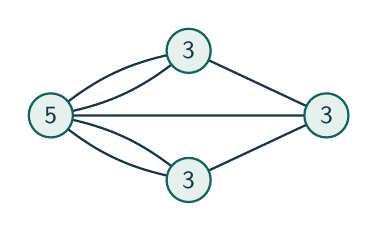
\begin{tikzpicture}[x=1cm,y=1cm,thick,draw=ink,every node/.style={font=\small\sffamily}]
\coordinate (a) at (0,0); \coordinate (b) at (1.75,.82);
\coordinate (c) at (1.75,-.82); \coordinate (d) at (3.5,0);
\draw (a) to[bend left=15] (b) (a) to[bend right=15] (b)
      (a) to[bend left=15] (c) (a) to[bend right=15] (c)
      (a) -- (d) (b) -- (d) (c) -- (d);
\foreach \p/\v in {a/5,b/3,c/3,d/3}
  \node[circle,inner sep=3pt,fill=lighttone,draw=accent,text=ink] at (\p) {\v};
\end{tikzpicture}\par
{\small Seven bridges, four odd degrees. No trail crosses every edge once.}
\end{center}
\vfill
{\sffamily\color{ink}Prepared for Vladimir Reshetnikov\par}
{\sffamily 22 November 2026\par}
\end{titlepage}
\hypersetup{pageanchor=true,bookmarksdepth=2}
\setcounter{page}{2}
\tableofcontents
\medskip
\noindent\textbf{Reading the collection.} The numbered sections form a self-contained manuscript. The three credited ProveIt companions extend the coverage of dimension, fixed points, and tangent fields. Section~\ref{sec:formal} gives the Lean targets, and Section~\ref{sec:sources} maps topics to their sources and precise scope.
\newpage
\section{What a topological assertion means in iPRA}\label{sec:arithmetic}
The number system is first-order intuitionistic primitive recursive arithmetic. Its axioms are the defining equations for the primitive recursive (PR) function symbols, the successor axioms, and induction for quantifier-free formulas with free numerical parameters. Outer universal and existential quantifiers and intuitionistic reasoning with hypotheses are available. The restriction is on the \emph{induction formula}. For example, the formula asserting that an arbitrary component of a space is connected should never be used as an induction invariant before the component and the connectedness test have been encoded.

There are two readings of the results below. A finite theorem, such as the assertion that every even grid chain has a filling, is a single number-theoretic assertion uniform in the size of the input. A theorem about a named continuum is a schema: substitute fixed PR routines for the names, maps, and moduli. Their numerical parameters remain free and may be quantified. A procedure constructed in the proof is a composition and iteration of those fixed routines. The implications from the advertised numerical contracts are genuine first-order formulas. None of this requires a universal total evaluator for PR codes: if $U(e,n)$ were such a PR function, the PR function $n\mapsto U(n,n)+1$ could not have an index in it.

\paragraph{A common encoding.}
Put $[n]=\{0,\ldots,n-1\}$. A subset of $[n]$ is a number below $2^n$, with membership given by binary digit extraction. A table of $r$ entries below $B$, with $B\ge2$, is a number below $B^r$; entry $i$ is $\lfloor a/B^i\rfloor\bmod B$. Store its length. Matrices of bits, families of subsets, flags on cells, signed words, finite lattices and graphs all use these conventions after fixing a row order. For variable-sized entries an alternative is the cons code $2^a(2b+1)$ for head $a$ and tail $b$, with zero as nil. Bounded division recovers both components; each tail is strictly smaller than the cons. Length, concatenation, and indexed reads have primitive recursive definitions. Ill-formed inputs receive default values, and theorem hypotheses test validity. The integer $z$ is coded by $2z$ if $z\ge0$, by $-2z-1$ otherwise. Rationals are a signed numerator and positive denominator. Cross multiplication decides equality and order, Euclid's division algorithm can normalize them (at most the sum of positive inputs many strict decreases). Norms, sums and products below involve finite rational vectors unless a name or approximation is explicitly indicated.

\begin{lemma}[Bounded decisions and witnesses]\label{lem:bounded}\label{idx-arithmetic9}
For a fixed PR bit test $P(i,u)$, the statements $\forall i<B\ P(i,u)=1$ and $\exists i<B\ P(i,u)=1$ have PR characteristic bits with provable introduction and elimination rules. In the existential case the first successful index is a PR term on success.
\end{lemma}
\begin{proof}
Scan $i=0,\ldots,B-1$, storing the first hit and a found bit. For a proof without a quantified induction invariant, fix a candidate index $j$ throughout. By induction on the scan length, if $j$ has already been seen and $P(j,u)=1$, the found bit is one and the stored witness is at most $j$. In a second quantifier-free invariant, when the bit is one the witness has been seen and its recomputed test is one. For the universal bit run the same search for a failed entry. If the resulting bit indicates success on every entry, specializing to each $j$ proves $P(j,u)=1$. Conversely the numerical hypothesis that all entries succeed rules out the recorded counterexample. Taking $B=0$ gives the usual empty conventions. Nest the construction to any fixed depth, allowing bounds to depend on earlier indices.
\end{proof}

\begin{proposition}[Finite loop reasoning]\label{prop:loops}\label{idx-arithmetic16}
Let $s(0,u)=a(u)$ and $s(i+1,u)=F(i,s(i,u),u)$, with $F,a,T$ PR. Suppose a quantifier-free invariant, possibly obtained by Lemma~\ref{lem:bounded}, holds initially and is preserved at every step $i<T(u)$. It holds at the terminal state and at every prior state.
\end{proposition}
\begin{proof}
Induct on the quantifier-free formula $i\le T(u)\Rightarrow I(i,s(i,u),u)$. At a successor within the bound the predecessor is within it and a permitted step yields the invariant. Substitute $T(u)$ or any smaller index. Several state registers can be paired. Recording all earlier states converts course-of-values computations of bounded length to ordinary primitive recursion. One may hold an input table fixed throughout, including when checking the same identity on all of its subfaces or rows.
\end{proof}

\paragraph{The step that requires proof.}
Giving a PR search bound establishes termination. It does not establish that the search succeeds. In the grid theorem the success argument is a parity identity. In the sphere contraction it is a bound on the number of roots of finitely many rational polynomials. In the homology computations it is a pivot invariant. These mathematical steps are where the restriction to iPRA must be checked. Quantifying over a fixed finite list of objects of unbounded-in-advance size is legitimate when each run produces its own bound. Reasoning over all names at once, replacing a cover by a finite one without data, or choosing an infinite coherent subsequence requires a separate argument.

\paragraph{Equality, apartness, and continuity.}
Equality of two names of a point will mean agreement to every prescribed accuracy. A positive distance certificate is stronger data than a negation of equality. We use a positive lower bound for division and a positive margin for side-of-curve decisions. Classical conclusions about all functions or all open covers do not automatically follow from the results for supplied PR presentations. Conversely, the finiteness of a description does not force its represented space to be discrete, finite, or of dimension zero. The manifold and homotopy constructions give examples.

\section{Finite spaces from their least neighbourhoods}
\label{sec:finite-spaces}

Consider the two-point space with opens $\varnothing,\{1\},\{0,1\}$.
Every open neighbourhood of $0$ contains $1$, whereas $1$ has a
neighbourhood missing $0$. Keeping track of this directional information
recovers the entire topology of every finite space. It also gives us small
witnesses for questions that the open-set description presents as
quantification over families.

\subsection{From a table of opens to a preorder and back}

Write $X=[n]=\{0,\ldots,n-1\}$. A subset is a bit mask $A<2^n$, a
family of masks is a mask $T<2^{2^n}$, and the complement $A^c$ is relative
to $X$. Test $T$ by checking membership of $\varnothing,X$ and checking
binary union and intersection of every pair of members. A scan starting at
$\varnothing$ and adding in each chosen member proves closure under the
union of every coded subfamily. A scan starting at $X$ proves the
corresponding intersection statement. During each scan the accumulator is
in $T$ and agrees, bit by bit, with the operation on the prefix. These are
bounded induction predicates. This also proves that complements of opens
contain $\varnothing,X$, are closed under coded intersections and finite
unions, and that taking complements again recovers $T$. Each subset used below is supplied as a mask or constructed from an
explicitly bounded decidable test.

\begin{theorem}[Finite specialization correspondence]\label{idx-finite26}
The tested topology tables on $[n]$ are in primitive-recursive bijection
with the reflexive transitive relations on $[n]$. In the convention used here
the opens are the upper sets. Refining the topology shrinks the relation.
\end{theorem}
\begin{proof}
Intersect the members of $T$ containing $x$ to obtain the open mask $N_x$.
It contains $x$, and a set is a neighbourhood of $x$ (contains an open
through $x$) exactly when it contains $N_x$. Put $x\preceq y$ when
$y\in N_x$. Reflexivity follows from $x\in N_x$. If $x\preceq y$ then
$N_x$ is an open containing $y$, so $N_y\subseteq N_x$. This proves
transitivity. For each open $U$, membership of $x$ forces $N_x\subseteq U$.
Conversely, a mask with that property is the union of $N_x$ over $x\in U$,
since each such $x$ belongs to $N_x$. Hence exactly the upper masks are open.
Starting from a preorder, the upper masks pass all the topology tests:
membership propagates along a relation edge in each union and intersection.
The principal upper set $\uparrow x=\{y:x\preceq y\}$ is upper by
transitivity and is contained in every upper set through $x$. It is
therefore $N_x$, proving the other round trip. For two tables $T,S$ on
the same carrier, $T\subseteq S$ implies $N^S_x\subseteq N^T_x$.
Conversely any mask upper for the larger relation stays upper when relation
edges are removed. This gives the refinement equivalence.
\end{proof}

The $N_x$ give a basis of at most $n$ opens. Any basis must contain each
distinct $N_x$: apply its covering property to $x\in N_x$, then use
minimality. More generally, let $\mathcal S$ be a finite table of proposed
subbasic masks. Define $x\preceq_{\mathcal S}y$ when every listed mask
containing $x$ contains $y$. This is a preorder. Its principal upper set at
$x$ is the intersection of the listed masks containing $x$, with empty
intersection $X$. Every topology containing $\mathcal S$ therefore contains
these principal sets and all their unions. Each listed mask is already
upper. Thus the preorder gives exactly the topology generated by the input
subbasis. In particular the two-point example has specialization $0\preceq1$.
On a labelled pair there are precisely four topologies: the empty and full
masks are forced, and either choice of membership for each singleton
passes the two tests.

\subsection{Interior, closure, boundary and dense sets}

\begin{theorem}[Local formulas and the closure axioms]\label{idx-finite66}
For any mask $A$ one has
\[
 x\in\operatorname{int} A\ \Longleftrightarrow\ N_x\subseteq A,
 \qquad
 x\in\operatorname{cl} A\ \Longleftrightarrow\
    (\exists y<n)\,[y\in A\ \land\ x\preceq y].
\]
Interior is the greatest open submask of $A$. Closure is the least closed
supermask of $A$, preserves binary unions and the empty set, is extensive,
monotone and idempotent. Interior preserves binary intersections and $X$,
is contractive, monotone and idempotent. The boundary consists precisely of
the $x$ for which $N_x$ meets both $A$ and $A^c$.
\end{theorem}
\begin{proof}
If $N_x\subseteq A$ and $x\preceq y$, then $N_y\subseteq N_x\subseteq A$.
Thus the first formula defines an upper mask, contained in $A$ by
reflexivity. Any open submask of $A$ that contains $x$ contains $N_x$,
proving maximality. Taking complements yields the second formula:
the finite scan for a member of $N_x$ in $A$ either produces a witness or
shows $N_x\subseteq A^c$. Closed masks are precisely lower masks.
The displayed witness formula for closure is lower by transitivity,
contains $A$ by reflexivity and is contained in every closed supermask
of $A$. A witness in $A\cup B$ supplies a witness in at
least one summand by testing its membership bit. No witness exists for
the empty mask. Inclusion preserves witnesses, and two successive
witnesses compose by transitivity. These observations give the four usual
Kuratowski axioms and monotonicity. Complement duality gives the interior
identities. Finally the boundary is $\operatorname{cl}A\cap
\operatorname{cl}(A^c)$; the witness formula proves the claim and also shows
that the boundary is closed. In particular it is empty exactly when $A$ is
both open and closed: at a point of $A$, the point itself witnesses the
first intersection test, so emptiness forces $N_x\subseteq A$, and the
same argument applies to $A^c$.
\end{proof}

Conversely, these closure axioms suffice to construct the entire topology.
Suppose a table $c$ on masks satisfies $c(\varnothing)=\varnothing$,
$A\subseteq c(A)$, $c(c(A))=c(A)$, and $c(A\cup B)=c(A)\cup c(B)$.
If $A\subseteq B$ then $B=A\cup B$ implies $c(A)\subseteq c(B)$. The
fixed masks contain $X$ and $\varnothing$ and are closed under binary
union. For any intersection $D$ of fixed masks, monotonicity puts $c(D)$
inside every factor, hence inside $D$, while extensivity gives the reverse
inclusion. Their complements are consequently a topology. Now $c(A)$ is
fixed and is contained in every fixed supermask of $A$, so it is exactly
the topological closure. The specialization matrix can be read directly
from $x\in c(\{y\})$.

\begin{proposition}[A minimum dense subset]\label{idx-finite114}
Identify points $x,y$ when $x\preceq y\preceq x$. A mask is dense exactly
when it meets each maximal equivalence class in the resulting finite
partially ordered set. Choosing the least numbered point in each maximal
class gives a dense subset of minimum cardinality.
\end{proposition}
\begin{proof}
The relation on classes is well defined by transitivity. Above any class
one can find a maximal class by moving to the least labelled strict
successor as long as one exists. A strict ascent cannot revisit a class
by antisymmetry. More explicitly, the number of classes strictly above
the current one drops at each move. Iterating $n$ times, with terminal
points fixed, suffices. If $A$ meets all maximal classes, the chosen
point of a maximal class above $x$ witnesses $x\in\operatorname{cl}A$.
Conversely a witness above a point of a maximal class must belong to that
class. Since the classes are disjoint, their chosen representatives give
the lower bound as well as a set attaining it (an injection into every
dense set selects its first member in each such class).
\end{proof}

\subsection{Maps, separation and classification by open sets}

\begin{theorem}[Continuity tests]\label{idx-finite136}
For a table $f:X\to Y$, each of the following characterizes continuity:
monotonicity for specialization, preservation of closed sets under inverse
image, and $f(\operatorname{cl}A)\subseteq\operatorname{cl}(f(A))$ for
every mask $A$. A bijection is a homeomorphism exactly when it preserves
and reflects the relation. Homeomorphism of two given finite spaces is
primitive-recursively decidable.
\end{theorem}
\begin{proof}
A monotone map takes upper sets to upper sets under inverse image. For the
converse, $f^{-1}(N_{f(x)})$ is an open through $x$, so it contains every
$y$ with $x\preceq y$. Thus $f(x)\preceq f(y)$. The closed-set test follows
by complementing preimages. Given monotonicity, carry a closure witness
$x\preceq y\in A$ to $f(x)\preceq f(y)\in f(A)$. Conversely apply the
closure condition to $A=\{y\}$ for every $x\preceq y$. Identities and
composites preserve the relation. A bijection has monotone inverse precisely
when it reflects the relation; its inverse table uses first-preimage search.
One can enumerate all forward tables on the carriers and retain exactly
those with the bijection and two relation tests. For domain size $n$ and
target size $m$, digits with radix $m+1$ give bound $(m+1)^n$ after checking
each digit is $<m$. This convention handles the empty carriers as well.
\end{proof}

\begin{theorem}[Separation, reflection, and the Sierpi\'nski space]\label{idx-finite159}
A finite space is $T_0$ exactly when its preorder is antisymmetric. The
conditions $T_1$, Hausdorff, and discrete are equivalent here. The quotient
identifying mutually comparable-in-both-directions points is $T_0$ and
is universal for maps to $T_0$ spaces. For finite $X$, opens of $X$ are in
bijection with continuous maps to the two-point space
$S=(\{0,1\},0\preceq 1)$. Every finite $T_0$ space embeds in a finite
power of $S$.
\end{theorem}
\begin{proof}
The $T_0$ test asks for an open containing exactly one of two distinct
points. When $x\not\preceq y$, $N_x$ is one; if both comparisons hold every
open has equal membership at $x,y$. All comparison bits are decidable.
The $T_1$ test requires an open through $x$ missing $y$ for each ordered
pair of distinct points, so $N_x=\{x\}$ for all $x$ and every mask is open.
Discrete spaces separate distinct points by disjoint singletons. Disjoint
neighbourhoods imply the $T_1$ test.

Represent the equivalence class of $x$ by $r(x)$, the least $y$ with
$x\preceq y\preceq x$, and retain the subset $R$ of representatives. For
representatives the restricted relation is antisymmetric. For all points
$x\preceq y$ is equivalent to $r(x)\preceq r(y)$ by transitivity, so
projection $r$ and inclusion $j:R\to X$ are monotone. Any monotone $f$
to a $T_0$ target takes equivalent points to equal points by antisymmetry.
The unique factor is $f$ restricted to $R$ because $rj$ is the identity.

Finally $\chi_U:X\to S$ is monotone precisely when $U$ is upper. Use the
coordinates $e(x)_a=\chi_{N_a}(x)$ for $a\in X$. Coordinatewise order
on the tuples gives $e(x)\le e(y)$ exactly when $x\preceq y$: monotonicity
gives one direction, and the coordinate $a=x$ gives the other. Antisymmetry
makes $e$ injective. The induced order on the image is the subspace order
by the construction below. This proves the embedding, including the empty
space.
\end{proof}

A separate example marks the role of the inverse-continuity hypothesis.
The identity from the discrete two-point space to $S$ is a continuous
bijection; its inverse fails monotonicity at $(0,1)$. For finite spaces a
continuous bijection to a Hausdorff target does have continuous inverse:
the inverse images of its open singletons are singleton opens throughout
the domain.

\subsection{Reconstructing the points from the lattice of opens}

For upper masks $U,V$, meet and join are intersection and union. Their
Heyting implication also has a finite formula:
\[
 U\Rightarrow V=\{x:(\forall y\in N_x)\,[y\in U\ \Longrightarrow\ y\in V]\}.
\]
This is upper since $x\preceq z$ implies $N_z\subseteq N_x$. For any open
$W$, if $W\subseteq U\Rightarrow V$ then $W\cap U\subseteq V$ by using
$y=x$ at each $x\in W\cap U$. Conversely, if $W\cap U\subseteq V$ and
$x\in W$, every $y\in N_x$ lies in $W$ and so $y\in U$ forces $y\in V$.
This proves the Heyting adjunction. In the two-point example the
pseudocomplement $\{1\}\Rightarrow\varnothing$ is empty, so the join of
this open with its pseudocomplement is a proper open.

\begin{theorem}[Finite distributive lattice representation]\label{idx-finite216}
Given the operation tables of a finite bounded distributive lattice $L$,
iPRA constructs a finite $T_0$ space whose open-set lattice is isomorphic
to $L$. Conversely the open-set lattice determines a finite $T_0$ space
and all its continuous maps: every bounded lattice homomorphism
$h:\mathcal O(Y)\to\mathcal O(X)$ between open-set lattices of finite
$T_0$ spaces is the inverse-image operation of a unique continuous
$f:X\to Y$.
\end{theorem}
\begin{proof}
Set $a\le b$ when $a\wedge b=a$. Scan the table for the nonzero elements
$j$ such that $j=u\vee v$ always entails $j=u$ or $j=v$ (the
join-irreducibles). Every such $j$ is join-prime: if $j\le a\vee b$,
distributivity gives $j=(j\wedge a)\vee(j\wedge b)$, hence $j\le a$ or
$j\le b$. Induction on the length extends this test to a finite join,
including the empty join since $j\ne0$.

Each $a$ is the join of all join-irreducibles below it. For $0$ this is the
empty join. If $a$ is join-irreducible, it is itself among the factors.
Otherwise search the operation table: since all the tests are decidable,
for $a\ne0$ there are $u,v$ with $a=u\vee v$ and $u,v<a$.
Each of these has fewer elements below or equal to it than $a$ does, since
its lower mask omits $a$. Induct up to $|L|$ on this lower-mask cardinality,
with the invariant testing the asserted join equation for all elements of
cardinality at most the counter. The joins for $u,v$ then give $a$; adding
any further irreducibles below $a$ cannot increase it beyond $a$.

Let $P$ consist of the join-irreducibles, ordered oppositely to $L$.
Then $a\mapsto D_a=\{j:j\le a\}$ is an upper mask on $P$. It preserves
meet by the definition of lower bound, and join by join-primality. It
preserves both bounds. It reflects equality by the join formula. If $D$ is
an upper mask of $P$, put $a=\bigvee D$ in $L$. Then $D\subseteq D_a$;
conversely any $j\in D_a$ is below some member of $D$ by the finite
join-prime test, so lies in $D$. This gives a computable inverse, also
when $L$ is the one-element lattice and $P$ is empty.

For the map statement and $x\in X$, intersect all opens $U$ of $Y$ with
$x\in h(U)$ to obtain an open $B$. This family includes $Y$, and
$x\in h(B)$ since $h$ preserves finite meets. Because $h$ preserves the
empty open, $B$ is inhabited. Write $B$ as the union of the $N_y$ over
$y\in B$. Preservation of finite joins gives a first $y\in B$ with
$x\in h(N_y)$. By the defining intersection $B\subseteq N_y$, and
$N_y\subseteq B$ since $B$ is open. Thus $B=N_y$ and antisymmetry
uniquely determines $y$ from $B$. Put $f(x)=y$. If $x\in h(U)$, then
$y\in B\subseteq U$. If $y\in U$, then $B=N_y\subseteq U$, so
$x\in h(B)\subseteq h(U)$; monotonicity of $h$ follows from meet
preservation. Thus $h(U)=f^{-1}(U)$ on every open, giving continuity.
For a second such function, the membership of its value in every open
would be identical, and $T_0$ forces the values equal. Applied to identity
and composite homomorphisms, uniqueness proves the stated reconstruction
up to isomorphism: in particular two isomorphic lattices give mutually
inverse continuous maps. All joins, meets, tests for irreducibles and
first-witness searches here scan bounded tables.
\end{proof}

\subsection{Building spaces and testing their universal properties}

\begin{theorem}[Subspaces, products, sums and quotients]\label{idx-finite273}
The induced topology on a mask $A\subseteq X$ corresponds to the restricted
preorder. The product preorder is coordinatewise, and the disjoint sum
preorder compares only points of the same summand. For a surjection
$q:X\twoheadrightarrow Q$, the quotient topology is given by the reflexive
transitive closure of
\[
 uEv\quad\Longleftrightarrow\quad
 (\exists x,y\in X)\,[q(x)=u,\ q(y)=v,\ x\preceq y].
\]
All four constructions and their map tests are primitive recursive.
\end{theorem}
\begin{proof}
For a point of $A$, its least relative neighbourhood is $A\cap N_x$.
Indeed any relative open through $x$ contains this intersection, which
is itself relative open. For the product, the rectangles of principal
neighbourhoods are precisely the principal upper sets of the coordinatewise
preorder. Every upper mask is a union of such rectangles, and every product
of opens is upper; this identifies the topology generated by open rectangles.
A table into the product is monotone exactly when each of its two projections
is monotone. In the sum the upper masks restrict to arbitrary upper masks
on the summands, proving the usual open-set test, and a table out of the
sum is monotone precisely when both restrictions are.

In the quotient, $q^{-1}(V)$ is upper if and only if membership of $V$
propagates along every $E$-edge. This holds if and only if it propagates
along every finite directed $E$-path by induction along that path. The
reflexive transitive closure can be computed by starting with the identity
and adding a last edge at each of $|Q|$ rounds, retaining all old pairs.
The invariant states that after $k$ rounds entries represent paths of
at most $k$ edges. Repeated vertices in a path allow the intervening
segment to be erased without changing its endpoints. Alternatively,
from each start the reachable mask grows strictly until stationary, so is
stationary by $|Q|$ rounds. A predecessor table at each round provides a
path for every positive entry. Therefore the ultimate matrix is transitive
and has exactly the upper masks prescribed by the quotient open-set test.
A function $h:Q\to Z$ is monotone exactly when $hq$ is: necessity uses
monotonicity of $q$, and sufficiency propagates monotonicity from the
generating edges along paths. In particular a monotone $f:X\to Z$ constant
on fibres factors uniquely; at $u$ use the first $x$ with $q(x)=u$.
\end{proof}

These rules also yield the pasting lemma for a coded finite cover of $X$
by open masks, or by closed masks. Given continuous functions on the
pieces which agree on intersections, take at $x$ the value on the first
piece containing it. Agreement makes this the common value on any such
piece. To prove monotonicity for $x\preceq y$, an open piece containing
$x$ contains $y$; in the closed-cover case a piece containing $y$ contains
$x$. On that piece use its monotonicity. This proves continuity and the
restriction property, which in turn gives uniqueness.

\begin{proposition}[Finite function spaces]\label{idx-finite324}
Let $Y^X$ be the mask of monotone tables $X\to Y$ among the radix-coded
candidates above, with $f\preceq g$ when $f(x)\preceq g(x)$ for each $x$.
Evaluation is continuous. For each finite $Z$ there is a bijection
between continuous maps $Z\times X\to Y$ and $Z\to Y^X$. This topology
on $Y^X$ agrees with its compact-open topology for finite $X$.
\end{proposition}
\begin{proof}
If $(f,x)\preceq(g,y)$, then $f(x)\preceq g(x)\preceq g(y)$; this
proves evaluation is monotone. For $a:Z\times X\to Y$ monotone, its row
$x\mapsto a(z,x)$ is monotone, and rows increase pointwise with $z$.
Conversely evaluating such a table of rows produces a monotone $a$.
Digit lookup shows the two operations undo each other. For the last
assertion a compact-open subbasic set consists of the functions sending
a specified compact mask $K$ into a specified open $U$. It is upper.
Conversely the principal upper set through $f$ is the intersection over
$x\in X$ of these subbasic sets for $K=\{x\}$ and $U=N_{f(x)}$.
Singletons are compact since any specified cover of one has a containing
member. Hence all principal upper sets belong to the compact-open topology.
\end{proof}

\subsection{Components, compactness and finite covers}
\label{sec:finite-components}

\begin{theorem}[Components and clopens]\label{idx-finite348}
Join two points by an undirected edge when either specialization comparison
holds. Reachability in this graph computes the connected components and
the quasicomponents. It produces either a zigzag between two input points
or a specific clopen mask separating them. Every clopen is a union of
components; if there are $c$ components there are exactly $2^c$ clopens.
\end{theorem}
\begin{proof}
Use the reachability algorithm of the quotient construction with the
symmetric edge relation. Its classes are both upper and lower: an
edge from or to a class member meets the same class. Each is therefore
clopen. Within a reachable class, any clopen for the induced topology is
both upper and lower along edges inside it. Its membership bit is constant
along each witnessing zigzag and hence across the class. This proves each
class is connected (has no nonempty proper relative clopen). Any connected
mask containing $x$ lies in its class, since intersection with the class
and its complement would otherwise give a nontrivial clopen partition.
The classes are therefore the maximal inhabited connected masks. The
quasicomponent at $x$ is the intersection of the clopens through $x$.
Such clopens contain the class, and the class itself is among them.

Assign disjoint indices to classes by their least representatives. The union
of the classes indexed by any bit mask is clopen and all clopens are
obtained exactly once, by testing their membership at each representative.
The empty space has no components and has its one clopen; it has no
separation into two inhabited opens. These conventions also show that a
space has no separation if and only if every pair of points is joined by
a zigzag.
\end{proof}

Continuous images of connected masks are connected: a monotone table sends
a zigzag in the restricted preorder to a zigzag inside the image. A product
of two connected inhabited spaces is connected: follow the first coordinate's
zigzag with second coordinate fixed, then follow the second coordinate's
zigzag with first coordinate fixed. If either carrier is empty the product
has no separation. In particular the clopen count and component count are
homeomorphism invariants. For a nonempty family of connected masks with a
given common point $p$, their union is connected, since each of its points
is joined inside its own mask to $p$. Here the family is a table and $p$
is part of the hypotheses.

\begin{proposition}[A sharp subcover bound]\label{idx-finite389}
For a finite space $X$, let $b$ be the number of minimal specialization
classes after passage to $T_0$. From any list of open masks covering $X$ one
can extract a subcover of length at most $b$; this bound is attained by
some cover. Every subspace satisfies the same theorem in its restricted
order. Closed subsets have the corresponding finite-intersection test.
\end{proposition}
\begin{proof}
Take the first representative of each minimal class and, by bounded search,
the first member of the list covering it. Each point lies above a minimal
class by the descending version of the strict-ascent argument. The selected
opens therefore cover; repetitions may be removed. The principal opens of
the minimal representatives form a cover, and none contains a different
minimal representative, so every member of that cover is indispensable.
If $X$ is empty the empty list suffices. Apply the same argument to the
relative preorder for any subspace. Complementing a list of closed masks
with empty intersection yields an open cover, and the selected at most
$b$ complements correspond to closed masks with empty intersection.
\end{proof}

For an indexed open family supplied by a fixed primitive-recursive
membership predicate together with a primitive-recursive selector assigning
a containing index to each point, the same proof takes the indices supplied
at the minimal representatives. For a finite table the selector is computed
from the table. This spells out which form of finite-space compactness
the arithmetic proof establishes, even when the outside indexing set is
presented as unbounded.

\subsection{A classification theorem for finite homotopy certificates}

A \emph{zigzag homotopy} from $f$ to $g$ is a list of monotone maps
$f=h_0,\ldots,h_s=g$ such that each consecutive pair is pointwise
comparable in one direction on the entire domain. This is a numerical
certificate: it equivalently gives a monotone map on $X$ times a finite
fence, the latter generated by an oriented edge between each pair of
successive list positions. The monotonicity check follows by changing
one coordinate at a time. Conversely restriction to the successive positions
gives the original certificate. Composition on either side preserves these
certificates. Reversing and concatenating lists proves symmetry and
transitivity.

There is a geometric interpretation of a certified comparison $f\preceq g$
in ordinary topology. Use the homotopy taking value $f$ at time $0$ and
$g$ at positive times. For an open $U$ its inverse image is
\[
  (f^{-1}U\times[0,1])\ \cup\ (g^{-1}U\times(0,1]),
\]
which is relatively open, and the restriction to either endpoint is as
claimed. This describes the inverse images directly, with no decision about
equality of a real name required by the certificate verifier. Reverse or
concatenate these homotopies for a whole zigzag. The arithmetic
classification below concerns the specified finite certificates. To see the
relation in the other direction in the usual interpretation, let $H$ be an
ordinary continuous interval homotopy between maps of finite spaces. Its
slices define a continuous map $s:[0,1]\to Y^X$: at any fixed $t_0$ the
inverse image of the least neighbourhood of $s(t_0)$ is the finite
intersection, over $x\in X$, of the open time sets on which
$H(x,t)\in N_{H(x,t_0)}$. Since each component of $Y^X$ is clopen,
the inverse image of the component of $s(0)$ is clopen and contains $0$.
Connectedness of the ordinary interval puts $s(1)$ in that component too.
The finite reachability algorithm then returns a zigzag. This comparison
uses the ordinary interval and its connectedness externally; the arithmetic
core proof below has only numerical inputs.

\begin{theorem}[Core reduction and rigidity]\label{idx-finite453}
In a finite poset call $x$ an upper beat point if its strict upper set has a
least element, and a lower beat point if its strict lower set has a greatest
element. Compute a core by passing to the $T_0$ representatives and deleting
beat points until none remain. Any such core is a retract of the given space
whose retraction followed by inclusion is zigzag-homotopic to the
identity. Two finite spaces admit mutually inverse maps up to zigzag homotopy
if and only if their cores are order isomorphic. This gives a
primitive-recursive decision and produces equivalence witnesses on success.
\end{theorem}
\begin{proof}
For the first reduction use $r,j$ from the separation theorem.
We have $rj=1$ and $jr$ is pointwise comparable to $1$ in both directions.
If $x$ is an upper beat point with least strict successor $y$, let $r$
fix the other points and send $x$ to $y$. Check an ordered pair
$a\preceq b$. If $a=x\ne b$, minimality gives $y\preceq b$; if
$b=x\ne a$, use $a\preceq x\preceq y$. Equality and the cases avoiding
$x$ follow at once. Thus $r$ is monotone, restricts to the identity on
the remaining subposet, and satisfies $1\preceq jr$. The lower case is
obtained by reversing every order comparison. The single comparison fixes
the remaining points. For successive deletions, composing the homotopy from
each step with the earlier inclusions and retractions gives the required
list; each earlier inclusion acts as identity on the ultimate subspace.
Tests for beat points and their witnesses scan pairs and all intermediate
points. Delete the least eligible point, preferring an upper deletion if
both tests pass, and iterate at most $n$ times. Alternatively any supplied
sequence of eligible choices gives the same properties.

Let $P$ be a beat-free finite poset and $h:P\to P$ monotone with
$1\preceq h$. If $h$ moves a point, choose a maximal moved point $x$ by
bounded ascent. For every $z>x$, maximality gives $h(z)=z$, so
$x<h(x)\preceq h(z)=z$. Then $h(x)$ is the least strict successor of
$x$, a contradiction. Because the set of moved points is a mask this proves
$h=1$. Dually $h\preceq 1$ also forces $h=1$. Along a list starting at
$1$, induction gives that every subsequent map is $1$. The prefix
invariant tests equality of two finite tables.

Given homotopy inverses between two original spaces, insert the
inclusions and retractions on both sides to get maps between their cores.
Their composites are zigzag-homotopic to the identities by composing the
certificates just constructed with the supplied maps. Rigidity makes both
composites actual identities. Thus these core maps are order isomorphisms.
Conversely, compose any isomorphism between two cores and its inverse with
the original retractions and inclusions. The displayed retraction
certificates verify the homotopy-inverse equations. The previous bounded
isomorphism search, followed by these explicit compositions, proves the
decision statement. Taking two reduction sequences on the same input gives
uniqueness of their cores up to isomorphism.
\end{proof}

For example, on a nonempty finite poset with least element the identity is
pointwise above the constant map to that element, so the space contracts in
one comparison. In contrast, take two incomparable minimal points each below
each of two incomparable maximal points. This four-point poset is connected
by zigzags. It has no beat points, since every nonempty strict upper or
lower set has two incomparable members. Its core has four points and
hence cannot be isomorphic to a singleton. It is connected and fails to
be contractible in the certificate model.

\begin{corollary}[Fixed points of finite-space maps]\label{idx-finite512}
A finite $T_0$ space has the property that every continuous self-map has a
fixed point if and only if its beat-free core has that property. In
particular every continuous self-map of a finite $T_0$ space that is
zigzag-contractible to a point has a computable fixed point.
\end{corollary}
\begin{proof}
For one deletion write $i:Y\to X$ for inclusion and $r:X\to Y$ for the
retraction. If $X$ has the property, apply it to $igr$ for $g:Y\to Y$.
Any fixed point belongs to $Y$ and there is fixed by $g$. Conversely,
suppose $Y$ has the property and let $f:X\to X$. Find a fixed point $y$
of $rfi$ by scanning $Y$. If $f(y)=y$ we are done. Otherwise $f(y)$
must be the deleted point $x$, and $y=r(x)$. For an upper deletion
$x<y$, so $f(x)\le f(y)=x$. Iterating $f$ from $x$ gives a descending
chain. Whenever a step changes value, the number of elements below or
equal to it strictly decreases, so at most $|X|$ iterations give a
stationary point. For a lower deletion reverse the inequalities.
This proves equivalence through the entire reduction. A contractible
$T_0$ space has singleton core by the rigidity theorem; the unique
self-map there has a fixed point. The $T_0$ assumption matters: both
points of the indiscrete doubleton are topologically indistinguishable,
and their transposition is a continuous fixed-point-free map although
the space contracts to either point by a single comparison.
\end{proof}

\subsection{Lean construction for the finite theorems}

At the numerical layer use \texttt{Nat} for each bounded table and use
\texttt{bit(n,A,i)} for membership, taken to be false when $i\ge n$.
Use \texttt{allBelow} and \texttt{anyBelow} by recursion on their bound.
Tabulate a predicate $p$ on $[k]$ by summing $2^i$ for the true indices.
An $n$-row relation uses bit $nx+y$, and a map is read by digit extraction
in radix $m+1$, with an explicit digit-range test. The following dependency
order gives the open proof obligations; names describe suggested Lean
declarations.
\begin{enumerate}
\item Prove \texttt{bit\_tabulate}, prefix specifications for the two
bounded scans, first-witness selection (with the bound as failure sentinel),
and digit-table extensionality for normalized codes. Define
\texttt{IsTopology}, \texttt{IsPreorder}, \texttt{upset}, \texttt{principal},
\texttt{specializes} and \texttt{opensOf} by the tests above. The invariant
for the defining intersection says a bit survives iff it survived every
selected mask in the processed prefix. This yields both round trips
by bit extensionality.
\item Define closure by witness search and interior with \texttt{allBelow}.
Prove the local formulas first. Then closure idempotence is a single use
of relation transitivity between the two chosen witnesses. Define
\texttt{MonotoneTable} by scanning ordered pairs. Use the mask
\texttt{principal (f x)} for the substantive direction of
\texttt{continuous\_iff\_monotone}.
\item Implement \texttt{reachStep} by adding endpoints of single edges
from the previous mask; retain for new endpoints their first predecessor.
Induct on the round to show that all recorded predecessors recover paths.
The cardinality of the current mask strictly increases if a new bit
appears; prove this by a scan counting bits. If a round adds nothing,
subsequent rounds repeat it. This proves stationarity at the carrier
bound. Applying the same routine to symmetric and directed edge tables
gives respectively the component and quotient constructions.
\item Use the least index in each equivalence class for the reflection,
count representatives, and implement product indexing by mixed radix.
Define currying and uncurrying by direct table lookup and prove their
equations entrywise. Select each cover index with first-witness search;
the minimum and maximum class searches use at most $n$ order steps.
\item For the lattice theorem, form the table of join-irreducibles by testing
all pairs. At stage $k$ verify the join reconstruction equation for all
$a$ whose lower mask has cardinality at most $k$. For the reconstruction
of a lattice homomorphism use the bounded intersection of qualifying opens
and extract the least principal open equal to this intersection.
\item Represent a homotopy certificate by a coded list of normalized
maps of the same dimensions. Verify each map and each adjacent comparison,
including equality at the endpoints. Implement \texttt{coreStep} on a mask
of surviving points, testing strict successors and predecessors only there.
Its invariant keeps a retraction, the inclusion and a list of maps from
the original identity to their composite. One deletion appends the new
composite, which is comparable to the preceding composite. The proof of
rigidity needs the bounded maximization of a moved point and induction
along the supplied list. Isomorphism of final cores is a search over maps,
with inverses computed on the surviving points or after increasing-order
reindexing. None of these loops needs induction on a formula with an
unbounded quantifier.
\end{enumerate}

\section{Metric topology at all precisions}
\label{sec:metric-names}

The source article says that a metric defines a topology, gives compactness and
connectedness as examples of invariants, and compares a cube and a sphere.
The linked articles on metric spaces and compact spaces also discuss completeness,
uniform continuity, finite nets, and extrema. Here the points themselves can carry
infinitely many approximations. Each approximation, each accuracy request, and
each construction used to answer it has an arithmetic meaning.

\subsection{Points and balls}

Use a coded countable dense domain $D$ with a primitive-recursive (PR)
rational metric $d$ and its three metric laws. The examples below are rational
vectors with $d(u,v)=\max_i |u_i-v_i|$, including the one-dimensional case,
and rational vectors in a cube. Write $e_p=2^{-p}$. A \emph{name} is a fixed PR
recipe $x_p\in D$, with its numerical parameters suppressed, satisfying
\[
 d(x_p,x_q)\le e_p+e_q\qquad(p,q\ge0).
\]
For a rational $a\ge0$ abbreviate by $D(x,y)\le a$ the arithmetic sentence
\[
 \forall p,q\quad d(x_p,y_q)\le e_p+a+e_q .
\]
Equality of points means $D(x,y)\le0$. Apartness means that some pair
$p,q$ violates the last inequality with $a=0$. A rational point is named by
its constant recipe. Quantifiers over names, dense-domain operations, or
moduli throughout this section specify theorem schemes, with their displayed
numerical assumptions as antecedents. In particular no number is evaluated as
the code of an arbitrary PR function.

\begin{lemma}[Error removal, density, and the metric laws]\label{idx-metric32}
If a rational inequality $b\le c+C e_h$ holds for every sufficiently large
$h$, with a given rational $C\ge0$, then $b\le c$. The relations
$D(x,y)\le a$ are symmetric and satisfy the triangle inequality in the sense
of adding bounds. Equality is an equivalence relation. Each $x_p$ is within
$e_p$ of $x$.
\end{lemma}
\begin{proof}
Decide the rational comparison. If $b-c>0$, write $b-c=u/v$ with positive
integer numerator and denominator. Take $h$ at least the given threshold and
at least $v(\lceil C\rceil+1)+1$. Then $2^h>vC$, which contradicts
the proposed inequality. For the triangle inequality bridge through the
$h$th entry of the middle name. This adds $2e_h$ to the desired rational
bound at fixed outer indices. Remove that error by the first assertion.
Reflexivity is regularity of a name, and symmetry comes from $d$. For density,
$d(x_p,x_q)\le e_p+e_q$ is precisely the required estimate against a
constant name (one may remove the constant name's extra error).
\end{proof}

\begin{proposition}[A countable basis and separation]\label{idx-metric51}
Rational balls form a countable basis on the named completion. PR-indexed
unions of presented opens and finite intersections of presented opens are
presented opens. Apart points have disjoint rational neighborhoods, and
failure of apartness implies equality.
\end{proposition}
\begin{proof}
A certificate for $x\in B(c,r)$ is an index $p$ with
$d(x_p,c)+e_p<r$. Passing to a different name for $x$ preserves membership:
at a sufficiently large stage $h$, the excess error $2e_h$ is smaller
than the displayed rational margin. The same calculation works for closeness
to a constant point: if $D(x,c)\le b<r$, taking $2e_h<r-b$ gives a
membership certificate.

Suppose $x$ belongs to two rational balls, with certificates for each.
Let $m>0$ be the smaller of their two rational margins, and take $h$ with
$4e_h<m$. The ball $B(x_h,2e_h)$ contains $x$ and lies inside both balls:
for each original center $c$, the triangle inequality gives
$d(x_h,c)+2e_h\le d(x_p,c)+e_p+3e_h<r$.
A presented open is a PR-indexed list of balls with a bit enabling each
entry. The empty list and the list of all balls present the empty and whole
spaces. To intersect two lists, enumerate triples of two enabled entries
and a rational ball $B(c,s)$ satisfying $d(c,c_j)+s<r_j$ for both entries.
These rational tests are decidable, and the refinement just proved shows the
result is exact. Use pairing of indices for a PR double list to take its union;
iterate the binary construction for any fixed finite number of lists.
For a uniformly given finite input family one can instead code all original
indices in a single tuple and make all its containment tests in a bounded scan.

For apart points take a certificate with rational surplus
$m=d(x_p,y_q)-e_p-e_q>0$. Balls at $x_p,y_q$ of radii $e_p+m/3,e_q+m/3$
contain the respective points and are disjoint, since their radii sum to less
than the distance of their centers. If no certificate exists, each individual
rational test for a violation fails by decidability. These inequalities give
equality. The weaker negative statement that two names are unequal does not
supply the positive margin used in the separation construction.
\end{proof}

\subsection{Completion and extension from a dense domain}

\begin{theorem}[Completion with a Cauchy modulus]\label{idx-metric91}
Let $x_{i,p}$ be a PR double array of names and $M$ a PR modulus such that
$i,j\ge M(k)$ implies $D(x_i,x_j)\le e_k$. Then a PR name $z$ satisfies
$D(x_i,z)\le e_k$ for every $i\ge M(k)$ and is the unique limit up to
equality. Thus the represented Euclidean space, and the represented closed
cube, are complete for such sequences.
\end{theorem}
\begin{proof}
Replace $M(k)$ by $\max_{j\le k}M(j)$ for constructing the name. Call this
larger bound $M^*(k)$ and put $z_p=x_{M^*(p+1),p+1}$. For $p\le q$ the
outer indices both exceed or equal $M(p+1)$, so
$d(z_p,z_q)\le 2e_{p+1}+e_{q+1}\le e_p+e_q$. For the stated convergence
use any $i\ge M(k)$ and fixed $s,q$. Bridge from $x_{i,s}$ to $z_h$ and
then $z_q$, with $h\ge k$. The bound is
$e_s+e_k+e_{h+1}+e_h+e_q$. Remove the vanishing errors.
Two limits with moduli are within $2e_k$ for every $k$ by bridging through
an index at least both convergence thresholds, giving equality.
All entries remain in the dense cube if the input entries lie there. A
coordinatewise bounded name may also be clipped to the closed cube at each stage:
clipping is 1-Lipschitz and moves a stage by at most its certified error if
the named point belongs to the cube. Componentwise clipping fixes the named
point by error removal.
\end{proof}

For the next theorem the source and target may have different rational
metrics. A map on the dense source consists of a PR array $A(u,p)$ forming a
target name for each $u$, together with a nondecreasing PR modulus $\mu$ such
that
\[
 d(u,v)\le e_{\mu(k)}\quad\Longrightarrow\quad D(A(u),A(v))\le e_k .
\]
A nonmonotone supplied modulus can first be replaced by its running maximum.

\begin{theorem}[Uniform extension and open inverse images]\label{idx-metric124}
There is a unique uniformly continuous extension to names, up to equality.
Its modulus can be taken to be $\nu(k)=\mu(k)+1$. Its inverse images of
presented opens are presented opens. Identity and composition preserve this
class of maps, and compositions have the composed moduli.
\end{theorem}
\begin{proof}
Put $n(p)=1+\max(p,\mu(p+1))$ and
$F(x)_p=A(x_{n(p)},p+1)$. For $p\le q$ and equal names $x,y$ the arguments
$x_{n(p)},y_{n(q)}$ differ by at most $2e_{n(p)}\le e_{\mu(p+1)}$.
The two target samples differ by at most $2e_{p+1}+e_{q+1}\le e_p+e_q$.
Interchanging the roles handles the other order of indices. This proves both
regularity and independence of representatives. On constant names the
reindexing $p\mapsto p+1$ preserves equality by regularity.

If $D(x,y)\le e_{\mu(k)+1}$, then at all sufficiently large $h$ the two
arguments at stage $n(h)$ differ by at most
$e_{\mu(k)+1}+2e_{n(h)}\le e_{\mu(k)}$. Hence their output samples at
stage $h+1$ differ by at most $e_k+2e_{h+1}$. Bridge to arbitrary fixed
outer samples by regularity and remove the errors depending on $h$. For
uniqueness compare two candidate extensions at $x$ through a rational
approximant $x_h$ within both input thresholds for target error $e_k$.
They agree there, so their outputs at $x$ differ by at most $2e_k$ for all
$k$. For composition use the computed target name as input to the next
extension and compose its accuracy requests in reverse application order.

For an output ball $B(b,r)$ enumerate every source ball
$B(c,e_{\nu(k)})$ with $c$ rational for which some stage $p$ gives
\[
 d(A(c,p),b)+e_p+e_k<r.
\]
Both $k$ and $p$ occur in the enumeration index. Uniform continuity proves
the containment in the inverse image. Conversely, if $F(x)\in B(b,r)$
its certificate gives a positive margin $m$. Choose $3e_k<m$ and $c=x_h$
with $2e_h<e_{\nu(k)}$. Then $x$ belongs to the enumerated candidate
source ball and $D(F(c),F(x))\le e_k$. At a sufficiently large stage $p$,
$d(A(c,p),b)+e_p+e_k\le r-m+2e_k+2e_p<r$. This certifies the entry.
Take the double union for any presented output open.
\end{proof}

\subsection{Grids, covers, and extrema}

\begin{theorem}[Quantitative compactness of a cube]\label{idx-metric166}
For $Q=[0,1]^d$ in the maximum metric and every $k$, the explicit grid
\[
 G_k=\{0,1/2^{k+2},\ldots,1\}^d
\]
is an open $e_k$-net of $(2^{k+2}+1)^d$ points. A ball cover with a
supplied local selection at one uniform scale admits an explicit finite
subcover. Uniformly continuous images of the cube are totally bounded.
\end{theorem}
\begin{proof}
Round each coordinate of the clipped stage $x_{k+2}$ down to the mesh of
$G_k$ by integer division. The rational rounding costs at most $e_{k+2}$,
so the named point is within $e_{k+1}$ of the returned grid point. This
leaves a strict margin for radius $e_k$.
Here is the precise cover input. For every $g\in G_k$ a given PR selector
(or a supplied table) returns an enabled index $j(g)$ of a ball $B(c_j,r_j)$
and $d(g,c_j)+e_k\le r_j$. Retain this finite list of indices. For each
$x$, the preceding rounding supplies a $g$ with $D(x,g)\le e_{k+1}$.
The triangle inequality gives a strict membership certificate in the selected
ball, because $e_{k+1}<e_k$. An actual uniform Lebesgue-radius selector,
valid at all rational centers, supplies precisely such a table on the grid;
larger original open sets can receive balls with certified inclusion.
The proof uses the uniform scale supplied with the cover.

For an image net at radius $e_k$, apply the grid construction at input scale
$\nu(k+1)$ and map its centers through $F$. Every image point is within
$e_{k+1}$ of one of these finitely many image points. If a net in the target
dense domain is desired, replace each image center by its rational stage
$k+2$, leaving a strict margin. The resulting rational centers need not
themselves belong to the image.
\end{proof}

\begin{proposition}[Deciding rational box covers and computing a Lebesgue radius]\label{idx-metric198}
\label{prop:boxcover}
Given a finite list of rational open boxes $B_i=\prod_{j=1}^{d}(l_{ij},u_{ij})$,
there is a PR test for whether their restrictions cover $[0,1]^d$. Failure
returns a missed rational point. Success returns a rational $\lambda>0$
and a PR selection from each named point $x$ of one original box containing
the entire relative ball of radius $\lambda$ about $x$. This applies in
particular to finite lists of rational open balls in the maximum metric.
\end{proposition}
\begin{proof}
In dimension zero the cube and every empty product are singletons.
If the list is empty return the empty tuple as a missed point; otherwise
use the first box and $\lambda=1$. Now let $d\ge1$. Discard boxes with
any $l_{ij}\ge u_{ij}$, retaining the original indices of the others.
For each coordinate $j$, sort the distinct numbers in the list $E_j$
consisting of $0,1$ and all endpoints in that coordinate, including
endpoints outside $[0,1]$. Within $[0,1]$ take each breakpoint itself
and the midpoint of each pair of consecutive breakpoints as representatives.
Test every tuple of representatives for membership in some retained box,
using strict rational comparisons. If any tuple fails, return it.
Otherwise every rational point is covered: replace each of its coordinates
by the representative of the same singleton or open interval. All strict
comparisons with original endpoints are preserved, including comparisons
at a face or corner of the cube. If there are $b$ original boxes, at most
$(4b+3)^d$ tuples are tested. In particular an empty list fails.

On success let $4\delta$ be the smallest positive difference between
consecutive members of any $E_j$. There is such a difference since
$0,1\in E_j$. For a rational point $v$ in the cube, snap each coordinate
within $\delta$ of a breakpoint to that breakpoint, leaving other
coordinates alone, to form $v'$. The candidate is unique when it exists.
It lies in $[0,1]$ because every breakpoint outside that interval is at
least $4\delta$ away from the nearer endpoint $0$ or $1$. Scan the boxes
for one containing $v'$. For every snapped coordinate both boundaries of
this box are distinct breakpoints from the snapped value and hence at least
$4\delta$ away from it. At the original coordinate they are at least
$3\delta$ away. An unsnapped coordinate was already more than $\delta$
from every breakpoint. Thus on every coordinate $v$ has slack at least
$\delta$ inside this one box.

Return $\lambda=\delta/2$. For a named point $x$, take a clipped rational
sample $v$ at a fixed stage $h$ with $2^{-h}<\delta/4$ (for example
$h=1+\lceil4/\delta\rceil$). Apply the preceding selection to $v$.
Every named point of the relative ball about $x$ is within
$\delta/4+\delta/2<\delta$ of $v$ in the maximum metric and therefore
belongs to that box, with a positive coordinate margin. Sorting, finding
the minimum gap and scanning the boxes use only finite rational data.
\end{proof}

\begin{corollary}[Extremal values with near-optimizers]\label{idx-metric247}
For a real-valued map $F$ as above on a nonempty cube the supremum and
infimum exist as PR names. At precision $p$ one can return a rational point
$q_p$ with $F(x)\le F(q_p)+e_p$ for every $x$.
\end{corollary}
\begin{proof}
Use $G_{\nu(p+2)}$ and form the rational maximum $m_p$ of stage $p+2$
output samples on that grid, retaining any maximizing index $q_p$.
Every sample differs from its named value by at most $e_{p+2}$.
Uniform continuity and rounding thus give
$F(x)\le m_p+2e_{p+2}$ for every $x$, whereas
$m_p\le F(q_p)+e_{p+2}$. The two errors sum to less than $e_p$.
In particular $m_p\le m_q+e_{p+2}+2e_{q+2}$ and the reverse estimate
holds with $p,q$ interchanged. Thus $(m_p)$ is regular. The inequalities
show by error removal that its value bounds $F$ above and lies below every
upper bound. Apply the same argument to $-F$ for the infimum.
Here and below an inequality between two scalar names is read at stages,
with the sum of the two stage errors allowed. This construction provides
the extremal value and the requested near-optimizer at each precision;
it supplies no convergence modulus for the sequence of optimizing points.
\end{proof}

The line already has a PR open cover with no finite subcover:
$B(0,n+1)$ for $n\in\mathbb N$. A first rational sample and its error
bound give an index covering each named point. For any finite nonempty
selection with largest index $N$, the rational $N+2$ lies outside all
selected balls. The empty selection misses $0$ as well.

\subsection{Paths, a discrete test for connectedness, and intermediate values}

\begin{theorem}[Contractibility and a connectedness test]\label{idx-metric277}
The cube is path connected and contractible by maps with explicit moduli.
Any PR coloring of its rational points by two bits that is locally constant
at every named point is constant. This last assertion requires no uniform
modulus of local constancy.
\end{theorem}
\begin{proof}
For two named points $u,v$ use $t\mapsto (1-t)u+tv$ for $0\le t\le1$.
For rational $t$ compute the indicated convex combination on the same
stages of both names. Its error against another such stage is bounded by
the same convex combination of the two error bounds. Varying $t$ costs
at most $|t-t'|$ since each coordinate difference in the unit cube has
magnitude at most one. Extension gives the entire path. Fix an anchor $a$
and put $H(x,t)=(1-t)x+ta$. Changing $x$ costs at most its displacement
and changing $t$ costs at most its displacement. Thus $k+1$ is a modulus
for the product maximum metric at target precision $k$. The endpoints
are the identity and the constant map, and $H(a,t)=a$.

For the second assertion, local constancy means that at every named $z$
there exist a positive rational radius and a bit such that every rational
point within this radius of $z$ has that bit. If two rational endpoints
have different bits, bisect their segment and query its rational midpoint.
Keep that half whose endpoint bits still differ. All choices are comparisons
of rational-point bits. After $n$ steps the endpoints are at distance at
most $2^{-n}$, and subsequent segments are contained in this segment.
The sequence of left endpoints therefore forms a PR regular name $z$, and
both endpoints of the $n$th segment are within $2^{-n}$ of it. These
assertions follow by bounded induction on intermediate subdivision steps:
each retained segment is a subsegment, and its length halves. Choose $n$
with $2^{-n}$ smaller than the radius supplied at $z$. Both endpoints must
now have the same bit, a contradiction. Thus all rational points have one
bit. A rational approximant to any $z$ in its local constancy neighborhood
has that same bit. This proves the claimed test. It rules out clopen
partitions whose side on rational inputs has a PR decision procedure and
whose local membership is witnessed on all named points.
\end{proof}

\begin{theorem}[Intermediate values and a fixed point at prescribed accuracy]\label{idx-metric314}
Let $F:[0,1]\to\mathbb R$ be given by the dense-domain array and modulus,
and suppose $F(0)\le0\le F(1)$. A PR construction returns $t_p\in[0,1]
\cap\mathbb Q$ satisfying $|F(t_p)|\le e_p$. If the actual values of $F$
on rational inputs are given by a rational-valued PR function, one can
instead construct a single named point $t$ with $F(t)=0$.
Every uniformly presented self-map of the interval consequently has
approximate fixed points, and the rational-valued-on-rationals case has
an exact named fixed point.
\end{theorem}
\begin{proof}
Put $s=p+2$ and $N=2^{\mu(s)}$. At $i/N$ for $0\le i\le N$
take an output sample $v_i$ of precision $s$. If $v_0\ge0$ then
$-e_s\le F(0)\le0$. If $v_N<0$ then $0\le F(1)\le e_s$.
In the remaining case scan for the first $i$ with $v_i\ge0$.
Its predecessor has $v_{i-1}<0$, hence $F((i-1)/N)\le e_s$.
The mesh and the dense-domain modulus give $F(i/N)\le 2e_s$,
while $v_i\ge0$ gives $F(i/N)\ge-e_s$. Return the indicated sample
point. Subtracting a target value reduces other intermediate values to zero
provided its name and the shifted evaluation scheme are supplied.

For exact rational evaluation bisect $[0,1]$. Keep $[a,m]$ when the
midpoint value is nonnegative, and $[m,b]$ otherwise. Each step preserves
$F(a)\le0\le F(b)$ and halves the length. The left endpoints give a PR name
$t$, within $2^{-n}$ of both endpoints of the $n$th interval. For every
$k$ choose $n\ge\nu(k)$; extension continuity and the two endpoint
inequalities give $-e_k\le F(t)\le e_k$. Error removal proves equality.
In this bisection the comparison at a possible zero is a decidable
comparison of rationals. For the fixed-point assertions apply the
corresponding construction to $t-F(t)$ with the displayed endpoint signs.
For a dense-domain modulus $\mu$ of $F$, the difference has modulus
$k\mapsto\max(k+1,\mu(k+1))$.
\end{proof}

\subsection{A cube boundary, a round sphere, and the open interval}

\begin{theorem}[Radial homeomorphism, uniformly in the dimension]\label{idx-metric350}
For $d\ge1$ the closed cube $[-1,1]^d$ and the closed Euclidean unit ball
are homeomorphic. The restriction takes the cube boundary homeomorphically
onto the unit sphere. In maximum-metric coordinates the forward and
inverse maps have Lipschitz constants at most $d+2$ and $3d$ respectively.
In particular the boundary of a square is homeomorphic to a circle.
\end{theorem}
\begin{proof}
Put $a(x)=\max_i|x_i|$ and $s(x)=(\sum_i x_i^2)^{1/2}$. The maximum and
the sum are finite folds. A square root of a nonnegative rational $v$ is a
regular name: halve $[0,1+\lceil v\rceil]$ repeatedly, testing whether
the rational midpoint squared exceeds $v$, and take an endpoint once the
interval length is at most $e_p$. At most $p+1+\lceil v\rceil$ halvings
suffice. The nested intervals give a unique nonnegative value of square $v$,
since the error in the square is bounded by twice the initial upper bound
times the interval length. For a nonnegative named scalar the same procedure
applies to its nonnegative rational sample at stage $2p+4$, using the
inequality $|\sqrt{u}-\sqrt{v}|\le\sqrt{|u-v|}$ (square both sides after
ordering rational inputs). Computing the rational sample's square root to
precision $p+2$ leaves total error at most $2e_{p+2}$.
Multiplication on a bounded interval is PR on names: bounds from the zeroth
samples plus one control the errors in each factor. To divide by a positive
quantity with rational lower bound $b$, clip denominator samples below at
$b$; the reciprocal changes by at most $b^{-2}$ times the sample error.
Thus the arithmetic below has PR realizers with bounded precision requests.

For rational $x\ne0$ define
\[
 P(x)=a(x)\frac{x}{s(x)},\qquad T(x)=s(x)\frac{x}{a(x)} .
\]
Set both values to zero at the rational origin. Each nonzero rational input
has the explicit lower bound $a(x)>0$ for both denominators. To extend
across the origin and to arbitrary named inputs we prove uniform estimates.
For rational $x,y$ write $\delta=a(x-y)$. We have
$|a(x)-a(y)|\le\delta$ and $a(x)\le s(x)\le d\,a(x)$ by summing squares.
Furthermore
\[
 |s(x)^2-s(y)^2|
 \le\sum_i|x_i-y_i|(|x_i|+|y_i|)
 \le d\delta\,(s(x)+s(y)).
\]
When either rational vector is nonzero there is a rational positive lower
bound on the sum in parentheses, giving $|s(x)-s(y)|\le d\delta$ by
division. If both are zero the inequality is immediate.

For nonzero $x,y$ set $N_s(x)=x/s(x)$. Writing the difference with first
denominator $s(x)$ and using $|y_i|/s(y)\le1$ gives
\[
 a(N_s(x)-N_s(y))\le(\delta+|s(x)-s(y)|)/s(x).
\]
Split $P(x)-P(y)$ into
$a(x)(N_s(x)-N_s(y))+(a(x)-a(y))N_s(y)$. Since $a(x)\le s(x)$ this
costs at most $(d+2)\delta$. The identical subtraction with
$N_a(x)=x/a(x)$ gives $a(N_a(x)-N_a(y))\le2\delta/a(x)$.
Split $T(x)-T(y)$ using $s(x)\le d\,a(x)$ and the bound on
$|s(x)-s(y)|$ to get $3d\delta$. With one argument zero use
$a(P(x))\le a(x)$ and $a(T(x))=s(x)\le d\,a(x)$.
A Lipschitz constant $L\ge1$ gives the PR modulus $k+\lceil L\rceil$.
Consequently both maps extend to all named vectors.

At a vector with a witnessed positive lower bound for $a(x)$ the extended
formulas agree with the displayed quotients: nearby rational approximants
have half the given lower bound, so the reciprocal estimate proves equality
by error removal. For rational nonzero $x$ one has $s(P(x))=a(x)$ and
$a(P(x))=a(x)^2/s(x)>0$, and direct substitution gives $T(P(x))=x$.
Likewise $a(T(x))=s(x)>0$ and $P(T(x))=x$. At the rational origin both
identities hold by construction. Equality on the dense rational domain
extends to all names by the uniqueness argument above. The identities
$s(P(x))=a(x)$ and $a(T(x))=s(x)$ extend in the same way. They show
exactly what happens to the closed unit sets and their boundaries.
No zero test on a named vector was used.
\end{proof}

There is also a quantitative version of the article's distinction between
the circle and the line. The boundary of $[-1,1]^2$ has four rational
edge grids of mesh $e_{k+2}$. For a boundary name $x$, take its clipped
stage $k+3$. A coordinate of largest absolute rational value is within
$e_{k+3}$ of magnitude one because $a(x)=1$. Move that coordinate to its
signed endpoint and round the other coordinate down on the edge grid.
The resulting point is within $2e_{k+3}+e_{k+2}<e_k$ of $x$.
The radial map therefore supplies finite nets on the circle. Any real-valued
map on it with a uniform modulus has bounded image: take a finite net at
the input accuracy for target radius one, and bound the finitely many center
values by the largest absolute zeroth sample plus one. Adding one bounds
the whole image. Thus no such map can be a surjection onto the line.
The uniform-modulus hypothesis here belongs to the representation.


\begin{theorem}[Two charts for the sphere]\label{thm:stereographic}\label{idx-metric438}
For $n\ge1$, each sphere $S^n\subseteq\mathbb R^{n+1}$ has two explicit
Euclidean charts. Each chart identifies the complement of one pole,
with positive separation from that pole, with the whole of $\mathbb R^n$.
The charts cover the sphere with a finite decision at one fixed precision.
Every $S^n$ is path connected. Finite products of these spheres are
path connected and have product Euclidean charts; in particular the torus
$S^1\times S^1$ has two-dimensional charts.
\end{theorem}
\begin{proof}
Write $x=(v,z)$ with $\sum v_i^2+z^2=1$. For
$\sigma\in\{1,-1\}$ the domain $U_\sigma$ consists of points with
a witnessed positive lower bound on $1-\sigma z$. This describes
positive separation from the pole $(0,\sigma)$:
the squared Euclidean distance to that pole is $2(1-\sigma z)$, and
the maximum and Euclidean norms bound each other as proved above. A
smaller rational lower bound on the same expression persists on a small
neighborhood, so the domain is relatively open. Put
\[
 \phi_\sigma(v,z)=\frac{v}{1-\sigma z},\qquad
 \psi_\sigma(t)=
 \left(\frac{2t}{1+w},\frac{\sigma(w-1)}{1+w}\right),
 \qquad w=\sum_{i=1}^n t_i^2 .
\]
The identity $4w+(w-1)^2=(1+w)^2$ puts $\psi_\sigma(t)$ on the sphere.
Its denominator gap at the excluded pole is $2/(1+w)>0$, so substitution
gives $\phi_\sigma\psi_\sigma(t)=t$. In the other direction the sphere
equation gives
$\sum_i (v_i/(1-\sigma z))^2=(1+\sigma z)/(1-\sigma z)$.
Both coordinates of $\psi_\sigma\phi_\sigma(v,z)$ now simplify to
$(v,z)$.

For inputs to $\phi_\sigma$ with denominator at least $b>0$, the maximum
norm displacement of the output is at most $(b^{-1}+b^{-2})$ times the
input displacement. This follows by subtracting the quotients and using
$|v_i|\le1$. Given a gap at one point, use half of it on a neighborhood.
For inputs of maximum norm at most $R$, say $R\ge1$, the change in $w$
is at most $2nR$ times the input displacement. The first coordinates of
$\psi_\sigma$ then have Lipschitz bound $2+4nR^2$. For the last coordinate
write $(w-1)/(1+w)=1-2/(1+w)$ to get the bound $4nR$. These bounds
supply all the local moduli, and bounds for $R$ come from zeroth samples
plus their error. The chart changes are compositions of these explicit
maps on their overlap. The relative rational balls of the ambient space
supply a countable basis and separate apart points.

To cover a given $x$, inspect the last coordinate's rational sample at
stage $2$. If it is nonnegative take $\sigma=-1$, and otherwise take
$\sigma=1$. In either case $1-\sigma z\ge3/4$. The equatorial point
$e=((1,0,\ldots,0),0)$ lies in both charts with coordinate
$e_1=(1,0,\ldots,0)$. In the selected chart join $\phi_\sigma(x)$ to
$e_1$ by linear interpolation, then apply $\psi_\sigma$. A numerical
bound on the two endpoints bounds the whole segment and gives a uniform
modulus for this path by the preceding estimates. To join $x$ to $y$,
follow the path from $x$ to $e$ and then the reverse of the path from $y$
to $e$. On rational times the two formulas are evaluated on the two
half intervals. Each is Lipschitz after rescaling time, and at times on
opposite sides the two bounds add through the common value at $1/2$;
the larger Lipschitz constant works on the whole interval. Extend from
rational times as above. For a finite product take paths coordinatewise.
The tuple of chart choices has open product domain (use the minimum of
the finitely many local radii); concatenating coordinate lists identifies
the chart target with Euclidean space in the sum of the dimensions.
\end{proof}

\begin{proposition}[Completeness depends on the metric]\label{idx-metric502}
The open interval $(-1,1)$ and the line have an explicit homeomorphism
with local moduli. With their usual metrics the line is complete for named
Cauchy sequences with modulus, and the open interval is incomplete.
\end{proposition}
\begin{proof}
Take $f(t)=t/(1+|t|)$ and $g(u)=u/(1-|u|)$. The first has
$1-|f(t)|=1/(1+|t|)>0$, with a rational lower bound obtained from the
zeroth sample of $t$. A name in the open interval comes with a positive
rational bound on $1-|u|$. Thus both divisions are available and the
identities $g(f(t))=t$ and $f(g(u))=u$ follow by substitution.
Absolute value is 1-Lipschitz. On $|u|,|v|\le1-b$ with $0<b\le1$,
subtracting the two quotients bounds $|g(u)-g(v)|$ by
$(b^{-1}+b^{-2})|u-v|$. Given a local gap, use half of it on a
neighborhood to obtain a local modulus. On $|t|,|v|\le R$ the same
subtraction bounds $|f(t)-f(v)|$ by $(1+R)|t-v|$.
These bounds give open inverse image neighborhoods in both directions.

The rational sequence $1-e_n$ lies in the open interval and its terms
at indices $i,j\ge k$ are within $e_k$. Its unique limit on the line is
$1$, since the distance of the $n$th term from $1$ is $e_n$. A limit
in the open interval would yield the same line limit and simultaneously
a positive gap from $1$, a contradiction.
\end{proof}

\paragraph{Lean implementation order.}
Use rational metric domains with a decidable carrier code and coded vector
length; implement comparisons on pairs of integers by cross multiplication
with positive denominators. Introduce transparent predicates
\texttt{Reg x}, \texttt{DistLE x y r}, and \texttt{BallMem x c r} using
the formulas above. Prove the rational error-removal lemma first, then the
bridge triangle, evaluation against constants, and the diagonal completion
lemma. For maps use fields for the rational-stage evaluator, its regularity,
the modulus, and the displayed dense-domain bound. Define extension by the
index $n(p)$ above and prove its regularity before its modulus or its
inverse-image formula. For total boundedness implement the grid index in
base $2^{k+2}+1$ and prove the rounding estimate coordinatewise. For
intermediate values implement the finite scan and the exact-sign
interval recursion separately. Prove nestedness between two given stages
by induction on their gap, with the initial stage fixed and stage comparisons
as Boolean tests. For the radial equivalence first implement rational
square-root brackets and division with a lower bound, then the two estimates
on rational vectors and finally uniqueness of extension. A Lean layer
may quantify over function-valued parameters for reuse. Each iPRA instance
instead substitutes fixed PR terms, keeps regularity and modulus laws as
hypotheses at the numerical indices queried, and uses induction on finite
loops with decidable invariants.

\section{Cantor space, gaps, and continuous images}\label{sec:cantor}
The Cantor set appears in the starting article. Its linked article
\emph{Compact space} gives the classical theorem that every nonempty compact
metric space is a continuous image of the Cantor set. We give the
arithmetical version for a dense rational metric domain with explicit finite
nets. An input point has a preimage computable from its name.

A binary stream $a$ is a fixed PR bit function with optional numerical
parameters. Write $a|n$ for its first $n$ bits, numbered from zero. A finite
word is its length together with its bit mask. The cylinder $[w]$ consists of
the streams with prefix $w$. Equality of streams means equality at each
index; apartness has a differing index as witness. Uniform continuity from
streams into a metric presentation means that agreement on the first
$L(k)$ bits guarantees output distance at most $2^{-k}$ for a supplied PR
function $L$.

\begin{theorem}[Clopen cylinders and finite prefix covers]\label{idx-cantor17}
Cylinders form a countable clopen basis. Distinct witnessed bits separate
points by complementary clopens. A connected subset contains at most one
point up to equality. There are no isolated points. Every finite list of
cylinders admits an exact cover test, with an explicit missed stream on
failure and a disjoint covering sublist on success.
\end{theorem}
\begin{proof}
Two cylinders intersect in the one with the longer prefix if their bits
are compatible, and otherwise are disjoint. The complement of $[w]$ is
the union of the other cylinders of length $|w|$. Finite intersections
and these complement formulas give the assertions about the product
topology whose basic restrictions fix finitely many individual bits:
any such restriction is a finite union of cylinders, taking the length
just past its largest restricted position. If two streams differ at $i$,
partition by bit $i$. Its two sides are finite unions of cylinders and
both meet the subset. Consequently, in a connected subset, for each fixed
$i$ the rationally decidable test of bit equality cannot fail, which proves
equality at every index. Flipping bit $n$ produces a distinct point in
$[a|n]$. Extending finite words by zeros also gives a countable dense list.

For words $W$ let $N$ be their maximum length, with $N=0$ for the empty
list. Enumerate all $2^N$ words of length $N$, asking whether each extends
an entry of $W$. A failing word followed by zeros misses every cylinder;
success proves coverage for any stream by reading exactly $N$ bits. Remove
duplicates and all words having a shorter listed prefix. This leaves the
same union, now disjoint. In the covering case each remaining $w$ accounts
for $2^{N-|w|}$ distinct length-$N$ words, so the retained words also
satisfy $\sum_w2^{-|w|}=1$. More generally, a PR predicate on words and a
given uniform hitting depth $N$ give a finite cover by scanning the words
of length at most $N$. Merely deciding the predicate does not supply this
depth.
\end{proof}

The $2^n$ zero-extended length-$n$ words give a finite net to precision
$n$ in the prefix topology. There is a complementary completeness
statement. Suppose a PR array of streams $a_i$ agrees in its first $k$ bits
whenever both row indices are at least the supplied $M(k)$. Define the
limit's bit $j$ to be bit $j$ of row $M(j+1)$. If $i\ge M(k)$ and $j<k$,
compare row $i$ with row $M(j+1)$ through the row indexed by
$\max(M(k),M(j+1))$. The first comparison preserves the first $k$ bits and
the second preserves the first $j+1$. Hence the limit has the required
convergence modulus. Uniqueness follows one bit at a time.

Similarly every represented continuous map from the interval to binary
streams is constant when for each output bit its evaluation on rationals
is PR and it is locally constant at every named input. Apply the cube's
bit-coloring theorem in Section~\ref{sec:metric-names} separately to each
bit. In particular the interval and Cantor set cannot be homeomorphic
by maps with these data, since the two constant streams have different
first bits.

\begin{theorem}[The middle-thirds embedding]\label{idx-cantor69}
Binary streams with the prefix topology and the named middle-thirds Cantor
set are uniformly homeomorphic. The latter is closed, perfect and nowhere
dense; it has finite interval covers of arbitrarily small total length.
The digit decoder works at the endpoints of all the deleted intervals.
\end{theorem}
\begin{proof}
For a word of length $n$ set
\[
 c(w)=\sum_{i<n}\frac{2w_i}{3^{i+1}},\qquad
 I_w=[c(w),c(w)+3^{-n}],\qquad C_n=\bigcup_{|w|=n}I_w .
\]
Children occupy the first and last thirds of their parent. Two different
level-$n$ intervals have distance at least $3^{-n}$: their first
different bit $i<n$ separates them by a middle gap of length
$3^{-(i+1)}$. For a rational $v$, distance to $C_n$ is the minimum of the
$2^n$ rational distances to the individual closed intervals; each distance
is $\max(0,c(w)-v,v-c(w)-3^{-n})$. It is 1-Lipschitz as a finite
minimum of 1-Lipschitz functions. For a regular name $x$ from
Section~\ref{sec:metric-names}, membership in the limiting set means
\[
          \forall n,q\quad \operatorname{dist}(x_q,C_n)\le 2^{-q}.
\]
A violation puts $x$ in the presented open complement: if the surplus is
$m>0$, a rational ball at $x_q$ of radius $2^{-q}+m/2$ contains $x$,
and is disjoint from $C_n$ by the distance estimate. Conversely enumerate
all rational balls with radius strictly below the center's distance to
some $C_n$. Membership in one yields a strict violation for a sufficiently
accurate sample. In particular membership in the Cantor set is the
negation of belonging to this open complement, since all individual
rational violation tests are decidable. This complement is the exterior
of $[0,1]$ together with the open middle thirds removed at the successive
stages. Indeed each finite-stage complement is exactly that finite list of
gaps together with the exterior; strict separation from its finite union
of closed intervals decides which gap by a sufficiently accurate sample.

Take $x_n=c(a|n)$. Subsequent sums lie in $I_{a|n}$ by the geometric sum,
so these left endpoints are a regular name with prefix error $3^{-n}$.
Each fixed interval $I_{a|n}$ contains the named point. Conversely,
given a name in the limiting set and a requested length $n$, take its
sample $x_h$ with $h=2n+3$ and select the word minimizing its distance
to $x_h$. For $n=0$ there is just the empty word. For $n>0$, its interval
is within $2^{-h}$ of the sample. At any $q\ge h$ the minimizing word
for $x_q$ must be the same: two different intervals would have distance
at most $2^{-h}+(2^{-h}+2^{-q})+2^{-q}\le4\cdot2^{-h}<3^{-n}$.
Thus at all such $q$ the selected interval is within $2^{-q}$ of
$x_q$. At earlier stages $p$, the triangle inequality bounds its distance
from $x_p$ by $2^{-p}+2\cdot2^{-q}$ for arbitrarily large $q$, and
error removal gives $2^{-p}$. This proves the interval contains the
named point. Uniqueness follows from the positive gap. Since a level
$n+1$ interval is contained in its level $n$ parent, the computed
words are compatible. Reading the last bit at each positive length
produces a single PR stream. The reconstructed point is within
$3^{-n}$ of its left endpoint at every level, hence equals the input.
The reverse composite preserves the unique prefix at every length.
Agreement of $n$ input bits bounds output displacement by $3^{-n}$;
input displacement in the real line strictly below $3^{-n}$ forces
the same $n$ output bits. These are moduli in the two directions,
and the estimates use no test of equality to a rational endpoint.

Closedness and the absence of isolated points give perfection, in the
sense that every Cantor point is a limit of other Cantor points: flip
bit $n$ to get distance between $3^{-(n+1)}$ and $3^{-n}$.
For any rational open interval take its midpoint $t$ and choose $n$
with $3^{-n}$ less than its radius. Decide whether $t$ belongs to a
level-$n$ interval. If not, a sufficiently small rational interval about
$t$ misses $C_n$ by a computed positive distance. If it does, the open
middle third of that level-$n$ interval lies inside the original interval
and misses $C_{n+1}$. Thus every basic open interval contains an open gap,
which proves nowhere density. Finally $C_n$ has an interval cover of total
length $(2/3)^n$. Choosing $n=2(k+1)$ gives total length strictly below
$2^{-k}$. If open covering intervals are required, enlarge each end by
$(2^{-k}-(2/3)^n)/2^{n+2}$. The enlarged total remains below $2^{-k}$.
\end{proof}

\begin{theorem}[A Cantor surjection from finite metric nets]\label{idx-cantor144}
Let $D$ be a nonempty PR rational metric domain. For each $k$ suppose
we have a nonempty finite PR list $c_{k,0},\ldots,c_{k,m_k-1}$ in $D$
such that every $u\in D$ is within $2^{-(k+4)}$ of a member.
Then binary streams map uniformly continuously onto the named completion
of $D$. Given any regular name $x$ one can compute a lifting stream.
\end{theorem}
\begin{proof}
Give proposals for stage $k$ a block of $b_k=\max(1,m_k)$ bits; this
simple choice ensures $2^{b_k}\ge m_k$. Read the block as an integer
modulo $m_k$ to propose a center $c_k$. Set $y_0=c_0$ and use the rule
\[
 y_{k+1}=\begin{cases}
 c_{k+1}&d(y_k,c_{k+1})\le2^{-(k+2)},\\
 y_k&\text{otherwise}.
 \end{cases}
\]
The test uses rational centers even when past proposals were rejected.
At any later stage the distance from $y_k$ is bounded by the finite
geometric sum of step bounds, hence by $2^{-(k+1)}$. Thus $(y_k)$
is a regular name. If two inputs agree through stage $k$'s block,
their outputs are within $2^{-k}$ by bridging through the common
$y_k$. The required prefix length is $L(k+1)=\sum_{j\le k}b_j$.

For a given target $x$, choose the first center within $2^{-(k+4)}$ of
the rational sample $x_{k+4}$ by scanning the supplied finite list.
It is within $2^{-(k+3)}$ of the named point. Two consecutive chosen
centers have distance at most $2^{-(k+3)}+2^{-(k+4)}<2^{-(k+2)}$.
Thus every proposal in this stream is accepted, and the output equals
$x$ by the error estimate. To compute bit $i$ of the stream, find the
unique $k$ with $L(k)\le i<L(k+1)$, where $L(0)=0$. Scanning at most
$i+1$ blocks suffices since every block has positive length. Output
the requested bit in the padded representation of the chosen center
index. This proves the lifting claim without a choice principle.
Different names for the same point may give different lifting streams.
\end{proof}

For instance the cube grids of Section~\ref{sec:metric-names} give these
nets uniformly in the dimension. The Cantor set therefore maps onto every
such cube, including the whole interval. This construction permits redundant
representations of a target, as its surjectivity proof requires. Interleaving
bits is itself a homeomorphism from a pair of streams to one stream: undo
it by reading even and odd positions. Finally no fixed PR double array lists
all PR streams, since $n\mapsto1-a_{n,n}$ differs from row $n$ at position
$n$. This is a diagonal theorem scheme about uniform enumerations.

\paragraph{Lean implementation.}
Represent $w$ by a natural bit mask and its length, with prefix, append,
test-bit and truncation. The coverage certificate is a bounded
\texttt{all} over masks below $2^N$, with a bounded \texttt{any} over the
input list. Define $3^n c(w)$ by appending digits to a base-three integer.
Prove the interval gap by the first differing bit, computed by bounded
search. Derive the decoder's universal containment only after proving the
rational nearest-interval estimate for two fixed precisions. For the
surjection define the offset $L$ by primitive recursion and store the
current rational center as the sole state of the acceptance recursion.
The quantitative invariant at two fixed stages is the rational geometric
sum bound. In the lifting proof the invariant that the accepted center
equals the proposed center at the current stage is decidable. The theorem
schemes have only numerical inputs once the stream, net and target-stage
recipes are fixed.

\section{Graphs, homology, and the surface table}
\label{sec:algtop}
The motivating article singles out the seven bridges, Euler's formula, and a
table of invariants of closed surfaces. These are three different kinds of
claim. A walk is a finite word, a homology computation is an identity about
integer or binary matrices, and the identification of an arbitrary space
with a particular surface requires a representation theorem. We prove the
first two directly. For surfaces we specify the presentations on which the
computations are performed.

\subsection{Paths and bridges}
A finite multigraph has vertices $0,\ldots,v-1$ and numbered edges
$0,\ldots,e-1$ with two specified ends each. The two ends may coincide.
An oriented edge is an edge number and a bit choosing its direction;
reversal flips that bit, even on a loop. A path stores its initial vertex
and a composable list of oriented edges. Degree counts ends with
multiplicity. Starting at a vertex, mark it, then repeatedly mark a new
vertex attached to a marked one, storing the attaching edge as its parent.
Stop at exhaustion or after $v$ passes, with one new mark per successful
pass. An edge cannot then lead from a marked to an unmarked vertex.
Induction along any given path proves it stays in the marked set. Parent
pointers, read in reverse marking order, give paths of length $<v$ to all
marks. Repeating from the least unmarked vertex gives a spanning forest
with exactly $v-c$ edges, where $c$ is the number of roots (components).
It has no cycle, since the last-marked vertex on a cycle would need two
earlier neighbors along forest edges. This argument counts a doubled edge
or a loop as a cycle when applicable.

\begin{theorem}[Euler trails and the seven bridges]\label{idx-algebraic29}
For a graph with at least one edge, an edge-once trail exists precisely
when all positive-degree vertices are in one component and the number of
odd-degree vertices is zero or two. In the former case the trail closes.
In the latter its endpoints are exactly the two odd vertices.
\end{theorem}
\begin{proof}
A trail connects every visited vertex to its start. Pair each arrival with
the next departure at an internal visit. All ends are paired except the
initial departure and terminal arrival, which also pair if the endpoints
coincide. This proves necessity. Suppose first all degrees are even.
Starting at an incident vertex, traverse the least unused incident edge
until there is none. Stopping anywhere other than the start would leave an
odd number of used ends at a vertex with no unused ends. Thus we have a
closed trail. Removing it preserves even degrees. If some edge is unused,
some visited vertex has an unused incident edge: otherwise no edge could
leave the visited set, and connectedness of the support would force every
incident vertex to have been visited and every edge used. Make another
closed trail from such a vertex in the residual graph, and splice it into
the first. Each splice uses a fresh edge. At most $e$ walks of length at
most $e$ suffice. With two odd vertices first join them by an extra edge.
Cut the resulting cyclic list at this edge and drop it. For the historical
bridge graph the four degrees are $5,3,3,3$ (one vertex has two edges to
each of two banks and one to the other island; each bank has one further
edge to that island). Its seven bridges therefore admit no such route.
\end{proof}

\begin{theorem}[The edge-path group of a graph]\label{idx-algebraic56}
At a root in a connected nonempty graph the group of based edge paths
modulo insertion and deletion of $a\bar a$ is the free group on
$e-v+1$ generators. Equality has a primitive-recursive normal form.
\end{theorem}
\begin{proof}
Read a word on signed letters with a stack, popping if the incoming letter
inverts the top and pushing otherwise. Its stack is reduced after every
step. Reading $a\bar a$ restores any reduced stack: if $a$ pops its
inverse, the exposed letter cannot be $a$, because the old stack was
reduced. In the other case the push is immediately undone. Thus insertion
and deletion preserve the answer in every context. Conversely the scanned
prefix is equivalent to its current stack, by induction on the scan. The scan records at most one adjacent-pair deletion per input letter,
so it also produces an explicit move transcript. This
proves the normal form theorem for free words (and the same argument
respects endpoints for edge paths).

Fix the parent tree and let $t_x$ be its route from the root to $x$.
Send a based path to its list of non-tree edges, oriented relative to
their given directions, then reduce. A generator corresponding to
$a:x\to y$ lifts to $t_xa\bar t_y$. Its inverse lifts to the reverse
loop. Projecting this lift gives the generator. Conversely insert
$\bar t_x t_x$ between consecutive edges at $x$ (each detour is obtained by nested
inverse-pair insertions) to write a based path as
a product of the lifted single-edge loops. For a tree edge its loop
cancels completely, since one endpoint is the parent of the other.
The constructions are inverse and concatenate modulo cancellation, which
also proves the group laws from the word operations.
Lifting a word of length $l$ uses at most $(2v+1)l$ edge symbols.
This is the combinatorial edge-path interpretation of the graph's
fundamental group; its definition here quantifies over finite paths and
moves.
\end{proof}

\subsection{Finite chain complexes and Betti numbers}
A simplicial complex on $v$ available labels is a table on the $2^v$
subsets, with the empty subset present and every subset of a present face
present. Labels absent as singletons are harmless. Order faces by their
bit masks. In degree $k\ge0$ the binary chain group $C_k$ consists of
masks on the $f_k$ faces of size $k+1$, with exclusive-or as addition.
In ordinary chains $d_0=0$. In positive degree, $d_k$ sends each face to
the sum of its one-vertex deletions and extends by addition. Write
$Z_k=\ker d_k$, $B_k=\operatorname{im}d_{k+1}$. For $k\ge2$ each
two-vertex deletion occurs twice in $d_{k-1}d_k$; for $k=1$ the
composite vanishes by $d_0=0$. Thus $B_k\subseteq Z_k$. Two cycles
represent the same homology class exactly when their sum is a boundary.

\begin{lemma}[Binary elimination with witnesses]\label{idx-algebraic103}
For an $m$ by $n$ binary matrix $A$, a bounded algorithm produces $r$
independent columns spanning the image, and $n-r$ independent kernel
vectors spanning the kernel. It also solves $Ax=y$ or detects failure.
\end{lemma}
\begin{proof}
Process columns in order. Store each surviving reduced column together
with the domain vector mapping to it. Give it the highest occupied row
as pivot. For the next column start with its domain unit vector; scan rows
from high to low, eliminating occupied old pivots by adding the stored
pair. If a nonzero residual has a new highest pivot, store it with its
domain vector. If the residual is zero, store its domain vector as a
kernel vector. (Eliminating all old pivots in one downward pass preserves
every cancellation above the row being processed.) The domain vectors
recorded after all columns, whether residuals are zero or nonzero, form a
basis: the vector for column $j$ contains bit $j$ and uses no later bit.
Descending elimination hence expresses any vector uniquely in this basis.
The nonzero residuals are independent because a largest pivot in a
nonempty sum survives. Consequently the zero-residual domain vectors span
exactly the kernel and the nonzero residuals span the image. To solve,
reduce $y$ in descending pivot order while accumulating the same domain
vectors. A nonzero remainder cannot be in the span because it contains no
pivot; a zero remainder exhibits a solution. If original independent
columns are desired, take the original column indices with nonzero
residual: at each such step subtracting a combination of earlier
residuals preserves the generated span and enlarges its dimension by one.
\end{proof}

\begin{theorem}[Euler--Poincar\'e and cohomology]\label{idx-algebraic131}
With $r_k=\operatorname{rank}d_k$, the ordinary homology classes have
unique binary coordinates of length
$\beta_k=f_k-r_k-r_{k+1}$. The same dimension is obtained for the
cohomology of the transposed boundary matrices. In particular,
\[
 \chi(K):=\sum_{k\ge0}(-1)^k f_k
        =\sum_{k\ge0}(-1)^k\beta_k .
\]
For subcomplexes $K,L$ on the same labels,
$\chi(K\cup L)+\chi(K\cap L)=\chi(K)+\chi(L)$.
\end{theorem}
\begin{proof}
Start a basis with the independent boundary vectors in $C_k$. Append
successively the computed kernel generators whose reduction is nonzero.
Keep the residuals and pivots as in the lemma. The final list spans the
kernel. Each cycle has unique coordinates in it, by descending pivot
elimination; two cycles differ by a boundary just when the appended
coordinates agree. A binary space with bases of sizes $a,b$ has both
$2^a$ and $2^b$ elements by unique coordinates, hence $a=b$ (alternatively
use elimination). The final list thus has length $f_k-r_k$. This yields
the claimed number of appended coordinates. For the transpose, the
domain change of basis in the elimination lemma puts $A$ in the form
consisting of independent image vectors and zeros. Extend these vectors
to a codomain basis by appending independent unit vectors. In these two
bases $A$ has exactly $r$ diagonal ones and remaining entries zero, up to
a permutation. Transposing the elementary invertible basis changes
preserves their invertibility, proving equality of ranks. Apply the same
kernel-quotient count to the transposed complex. In the alternating sum
the two appearances of each nonzero boundary rank cancel, including the
end cases since $d_0=0$ and degrees above $v$ vanish.
Inclusion--exclusion follows by testing membership of each nonempty face
in the two tables.
\end{proof}

\begin{corollary}[Graphs and degree zero]\label{idx-algebraic166}
For a finite complex $\beta_0$ is the number $c$ of components of its
vertex-edge graph. For a finite graph, allowing loops and repeated edges
by using their binary incidence columns, $\beta_1=e-v+c$ and
$\chi=v-e$.
\end{corollary}
\begin{proof}
Each edge boundary has even total parity in each component. Conversely
the boundary of a parent route from $x$ to its root is the pair of
endpoints (zero when they coincide). Summing these routes over the marked
bits of a vertex chain with even parity in each component reproduces that
chain as a boundary. The component parities are independent since each
root is a representative. Thus $r_1=v-c$. A graph has $d_2=0$, proving
the degree-one formula.
\end{proof}

\subsection{Cones, spheres, and invariance under subdivision}
Use the augmented complex temporarily, adjoining one empty face in degree
$-1$, with $d$ of a vertex the empty face and $d$ of the empty face zero.
This is an index shift of a finite list of matrices. For any simplicial
cone with apex $u$ (that is, $s\cup\{u\}$ is present for every face
$s$), let $h(s)$ adjoin $u$ if absent and be zero if present. If $u$ is
absent, its deletion from $h(s)$ gives $s$, and deleting any other vertex
matches a summand in $hd(s)$. If $u$ is present, only its deletion in
$hd(s)$ contributes. This includes the empty face. Hence
$dh+hd=1$. In particular a reduced cycle $z$ has filling $h(z)$.

\begin{theorem}[Simplex and boundary sphere]\label{idx-algebraic193}
The full simplex on $n+1$ vertices, $n\ge0$, has vanishing reduced
binary homology. For $n\ge1$, its boundary has reduced homology of
dimension one in degree $n-1$ and zero elsewhere. The top cycle is the
sum of its facets. In particular a triangle boundary has ordinary Betti
numbers $(1,1)$, and a tetrahedral boundary has $(1,0,1)$ and
$V-E+F=2$.
\end{theorem}
\begin{proof}
The full simplex is a cone. A reduced boundary-sphere cycle $z$ of
degree $k<n-1$ fills by the cone formula in the full simplex; its filling
still has degree below $n$, so uses only proper faces. In degree $n-1$
the cone filling is a multiple of the unique $n$-simplex, so every
cycle is a multiple of its boundary. That boundary has distinct facets,
is nonzero, and has no possible filling among the proper faces. In
higher degrees there are no chains. For a nonempty complex, sorting a
vertex chain by its parity splits off the class of a chosen vertex in
ordinary degree zero, leaving reduced degree zero; positive degrees are
unaffected.
\end{proof}

A simplicial vertex map sends a face to a face as an unordered image. On
chains let $F$ send a basis face to its image if the vertices remain
distinct and to zero otherwise. It sends the empty face to itself.
It commutes with $d$: for an injectively mapped face, deletions match
bijectively. If the image has deficit one, only the two deletions from
the duplicated pair give nonzero terms, and their images agree. With
larger deficit every deletion still has a repetition. This rule
respects identity and composition since repeated images cannot regain
distinctness under a second map. A chain map therefore sends cycles to
cycles and boundaries to boundaries, inducing a map on homology. The
algorithm above supplies its matrix by reducing the images of class
representatives.

\begin{lemma}[A cone filling for chain homotopies]\label{idx-algebraic227}
Suppose augmentation-preserving chain maps $F,G$ from a simplicial
complex to another are carried by cones $Q(s)$: both images of each
nonempty basis face $s$ are supported there and
$Q(t)\subseteq Q(s)$ for nonempty $t\subseteq s$. Then there is a
computed family of binary matrices $P$ of degree $+1$ such that
$dP+Pd=F+G$. In particular $F,G$ induce the same map on homology.
\end{lemma}
\begin{proof}
Put $P(\varnothing)=0$. In increasing face size set
\[
 P(s)=h_{Q(s)}\bigl(F(s)+G(s)+P(d s)\bigr).
\]
The chain in parentheses lies in $Q(s)$ by the containment condition and
the previous steps. Its boundary is zero: use the two chain map
identities and $dP(d s)=(F+G)(d s)+P(d^2s)$, already established on
proper faces (including the empty face). Hence its cone filling has the
asserted boundary. Extending additively proves the identity. On an
ordinary positive-degree cycle the difference of images is the boundary
of $P(z)$; in degree zero the same conclusion holds since
$P(\varnothing)=0$.
\end{proof}

\begin{theorem}[Contiguity, elementary collapse, and subdivision]\label{idx-algebraic250}
Contiguous simplicial maps induce equal maps on homology. Removing a
maximal simplex $s$ together with a nonempty codimension-one face $t$
having no other proper coface preserves homology. Barycentric subdivision
induces a computable isomorphism on homology in all degrees.
\end{theorem}
\begin{proof}
Contiguity means that the union of the two images of each face is a face.
Take $Q(s)$ to be the full simplex on that union and apply the cone
lemma. Consequently a finite chain of contiguities gives the same map;
mutual inverse maps up to such chains induce inverse homology maps.

For a collapse write $d s=t+b$, where $b$ uses only remaining faces.
The projection to the remaining chains fixes these, sends $s$ to zero,
and $t$ to $b$. It commutes with $d$ since $d b=d t$ and $t$ occurs
in the boundary of no other simplex. Its composite with inclusion is
the identity on remaining chains. On the original chains the difference
from the identity is $dP+Pd$ with $P(t)=s$ and $P=0$ elsewhere, as
one sees on $s,t$ and each remaining face. This also proves invariance
for a supplied finite sequence of collapses or their inverses.

Vertices of $\operatorname{sd}K$ are the nonempty faces of $K$, and
its simplices are strictly increasing chains of such faces. On augmented
chains define $S(\varnothing)=\varnothing$ (the basis vector).
Given a nonempty face $s$, cone $S(d s)$ to the vertex $s$ in
$\operatorname{sd}(2^s)$, the subdivision of the full simplex on $s$.
This complex is a cone since every chain can be extended by $s$ unless
it ends there. By induction $S(d s)$ is a cycle in that cone and its
filling has boundary $S(d s)$, so $S$ is a chain map with the indicated
support. Map a subdivision vertex $t$ to the greatest original vertex
of $t$. This assignment is simplicial since all images of a chain
belong to its largest face. Call its chain map $L$. The maps $LS$ and
the identity on $K$ are carried on $s$ by the full simplex on $s$.
The maps $SL$ and the identity on $\operatorname{sd}K$ are carried on
a nonempty chain ending in $s$ by $\operatorname{sd}(2^s)$.
These carriers are nested under taking faces. Apply the lemma twice to
obtain inverse homology maps. Iteration along any supplied finite list of
subdivisions or simplicial isomorphisms preserves the calculated groups
and Euler characteristic.
\end{proof}

\subsection{Euler's formula for a rational convex polyhedron}
A vertex presentation lists distinct points $p_1,\dots,p_m$ in
$\mathbb Q^3$ of affine dimension three. With each $p$ it gives a
rational covector $u_p$ with $u_p(q-p)>0$ for all other points $q$.
This certificate ensures that every listed point is a vertex. The
polyhedron means their convex hull. Its facets are the maximal lists
in a supporting plane spanning that plane, and its edges are its
exposed segments. These data can all be tested with rational arithmetic.
In particular supporting facet candidates are enumerated by triples.
Here convex combinations can be read throughout as rational ones.

\begin{lemma}[Planar sections of a finite hull]\label{idx-algebraic302}
For noncollinear rational points in a plane, their hull has a boundary
polygon. A rational affine form $x$ taking distinct values at the points
splits its boundary into two chains from the least to the greatest
$x$, along which $x$ increases. Consequently a cut $x<a$ avoiding the
polygon vertices selects one consecutive cyclic block of vertices, unless
it selects all vertices or none.
\end{lemma}
\begin{proof}
Use $x$ as the first affine coordinate and take an independent rational
coordinate $y$. At each rational abscissa $t$ between the extremes, the
possible ordinates form the interval between the lowest and highest
ordinates obtained by interpolating pairs of the given points spanning
$t$ (include a point at $t$). Indeed, in a convex combination with
three positive coefficients there is a nonzero rational change of those
three coefficients preserving their sum and their weighted sum of $x$.
It has both signs. Choose its sign so that the weighted $y$ does not
decrease, and move until a coefficient first becomes zero. Iterate at
most the size of the support to get an upper bound from a pair. For a
lower bound reverse the choice of sign. The extreme ordinates are
attained and all intermediate ordinates are mixtures of the two.
The resulting upper envelope is concave by taking mixtures of its
maximizers. Between successive input abscissae the candidate segments
are fixed, so the upper envelope is also convex there as a maximum of
affine functions. It is therefore affine on each such interval.
There is no jump at an interior input abscissa, by the concavity
inequality using points on both sides; at either extreme the finitely
many candidate segments reaching it share the unique endpoint.
The lower envelope has the reversed argument. Noncollinearity makes
the two envelopes distinct at every interior abscissa: an interior
triangle has positive vertical thickness at some abscissa, and mixtures
with either endpoint propagate positive thickness throughout the
interior. Removing collinear intermediate points leaves two strictly
$x$-monotone polygonal chains, meeting only at their ends. Each corner
is an input point: an extremizer at a corner supported by two different
abscissae would, by concavity (or convexity), force the same affine
segment on both sides. Each resulting side has a supporting line, as
follows by monotonicity of the slopes of a concave or convex function.
These two chains give the asserted cyclic block rule.
\end{proof}

\begin{theorem}[Euler's polyhedron formula]\label{idx-algebraic343}
For a full-dimensional rational convex vertex presentation,
$V-E+F=2$, with polygonal faces counted before any triangulation.
\end{theorem}
\begin{proof}
At $p$ form the planar hull $Q_p$ of the normalized directions
$q'=(q-p)/u_p(q-p)$, lying in $u_p=1$. It is two-dimensional since the
rays span three-space. Its points $q'$ are distinct: two on the same
ray would make the nearer input vertex a strict convex combination of
$p$ and the farther one, contradicting its exposing certificate.
Every affine form on $u_p=1$ extends to a linear form on the ambient
vector space (extend its constant using $u_p$). Thus a supporting line
of $Q_p$ gives a supporting plane of the original hull through $p$.
A corner of $Q_p$ is exposed by the sum of inward slacks of its two
incident sides, giving exactly one edge from $p$. Conversely an exposed
edge from $p$ must expose just one of the normalized directions, a corner.
A side of $Q_p$ gives exactly one facet through $p$: its two extreme
directions span a plane with $p$, and all its directions give exactly
the input vertices on that plane. Each facet through $p$ gives a side
in reverse. This proves the incidence correspondence used below.

Choose a rational linear height $h$ separating the input vertices and
also separating all pairs of normalized directions within each $Q_p$.
Testing $(1,j,j^2)$ for $j=0,1,\ldots,2M$ suffices for $M$ pairwise
inequalities to avoid: each nonzero difference gives a nonzero polynomial
of degree at most two with at most two integer roots. Heights of the
normalized directions are nonzero, with the sign of $h(q)-h(p)$.
At $p$ count $1$ for the vertex, subtract $1$ for each edge pointing
downward from $p$, and add $1$ for each facet whose greatest vertex is
$p$. The latter facets correspond to sides of $Q_p$ with both ends
negative, because every direction on the side is a mixture of its ends.
These contributions count each edge and each facet exactly once globally.

If all corners are positive, all normalized directions are positive by
convexity and $p$ is the global minimum. Its contribution is $1$.
If all are negative, $p$ is the global maximum and its contribution is
$1-k+k=1$, for $k$ corners. In the mixed case let $k$ be the number of
negative corners. They form one consecutive proper block by the planar
lemma for $x=h,a=0$, and exactly $k-1$ sides have both ends in it. The
contribution $1-k+(k-1)$ vanishes. There is one global minimum and one
global maximum, proving the formula. The planar argument uses at most
all pairs of points per envelope ordinate. Affineness reduces each
inequality about an interpolated interval to its endpoints. Thus the
sweep needs only bounded lists and rational operations in iPRA.
\end{proof}

\subsection{The integer homology and orientability of the polygon models}
Work now over $\mathbb Z$. Use $g$ handles and $c$ cross-caps in the
standard polygon word
\[
 w=\prod_{i=1}^{g}a_ib_ia_i^{-1}b_i^{-1}
       \prod_{j=1}^{c}y_jy_j .
\]
The formula below concerns the polygon with paired edges indicated by
this word, including the orientable models $c=0$ and the nonorientable
ones $c>0$. The empty word is handled by the tetrahedron boundary.
No recognition or classification algorithm for an arbitrary supplied
surface is needed.

\begin{theorem}[The surface table over the integers]\label{idx-algebraic402}
Write $m=2g+c$. The connected polygon model has Euler characteristic
$2-m$. Its homology in degrees $0,1,2$ is respectively
\[
\begin{array}{c|ccc}
 &H_0&H_1&H_2\\ \hline
 c=0 &\mathbb Z&\mathbb Z^{2g}&\mathbb Z\\
 c>0 &\mathbb Z&\mathbb Z^{m-1}\oplus\mathbb Z/2&0 .
\end{array}
\]
It is orientable exactly when $c=0$. In particular the sphere, torus,
and double torus have $(b_0,b_1,b_2)=(1,0,1),(1,2,1),(1,4,1)$.
The projective plane and a Klein bottle model have $(1,0,0)$ and
$(1,1,0)$ respectively, each with one order-two summand in degree one.
\end{theorem}
\begin{proof}
Suppose the word has length $l>0$. All boundary vertices are identified:
in a commutator block with successive corners $0,1,2,3,4$ the first
pair gives $0=3,1=2$ and the second gives $1=4,2=3$. In a square
block the two copies identify all three corners. Blocks share endpoints.
Call the common vertex $p$, add a center $o$, and draw $l$ spokes
$r_i:o\to p$ to successive corners ($i$ modulo $l$). These are
distinct numbered edges. Let $e_j$ denote the oriented edge for each of
the $m$ distinct boundary letters. The oriented triangle between spokes
$i,i+1$ has boundary
\[
 dT_i=r_i+s_ie_{j(i)}-r_{i+1},\qquad
 dr_i=p-o,\quad de_j=0 ,
\]
where $s_i$ is the sign of the letter. This is the ordinary oriented
triangle-edge-vertex incidence complex of the glued fan, with face
identifications allowed. There are $2$ vertices, $m+l$ edges and $l$
triangles. This proves the Euler count and $H_0=\mathbb Z$.

A $1$-cycle has total spoke coefficient zero, so its unique coordinates
are the $e_j$ and $q_i=r_i-r_0$ for $1\le i<l$. Put $q_0=q_l=0$.
The boundary relations are $q_{i+1}=q_i+s_ie_{j(i)}$. Successive
substitution eliminates all $q_i$ leaving just
$u=\sum_i s_i e_{j(i)}=0$. Explicitly, replace each $q_i$ by the prefix
sum up to index $i-1$, using the first $i$ triangle boundaries.
These substitutions kill the first $l-1$ relations and send the last
one to $u$; conversely $u=\sum_i dT_i$. Thus a cycle is a boundary
exactly when its final $e$-vector is an integer multiple of $u$.
The spoke coefficients of $d\sum_i t_iT_i$ vanish exactly when
$t_i=t_{i-1}$ for every $i$. The remaining boundary is then $t_0u$.
There are no $3$-chains. For handles alone $u=0$, giving the first
row. With cross-caps, $u=2(y_1+\cdots+y_c)$, where letters now denote
basis vectors. Replacing $y_1$ by $y_1+\cdots+y_c$ is an invertible
integer basis change with inverse obtained by subtraction. The new
coordinate is reduced modulo two, proving its exact order and both
homology formulas. A consistent orientation chooses $t_i\in\{1,-1\}$
for every triangle with paired edge incidences cancelling. The spokes
force a single sign throughout, which succeeds precisely when the
paired boundary incidences have opposite directions, i.e. $c=0$.

For the empty word use the tetrahedral boundary with oriented faces
and alternating deletion signs. In the full simplex, prefixing the
least vertex if absent (and returning zero otherwise) gives
$dh+hd=1$ on augmented integer chains: deletion of the prefixed vertex
has positive sign, and the signs of all later deletions reverse. When
the least vertex is already present only its deletion contributes to
$hd$. The preceding simplex-boundary proof now works over $\mathbb Z$,
giving the sphere row. Its signed facet boundary supplies a consistent
orientation. Finally the usual Klein bottle polygon can also be read as
$a b a^{-1} b$; its paired corners are all identified and its exponent
vector is $2b$, so the same spoke calculation proves its stated row
directly.
\end{proof}

\subsection{Finite filtrations and their barcodes}
Let $K_0\subseteq\cdots\subseteq K_N$ be finite face tables on common
labels. In any fixed degree, the preceding algorithms turn the inclusions
into binary matrices $A_i:V_i\to V_{i+1}$ on ordinary homology
coordinates. Examples include the proximity complexes of a finite
rational metric space, whose face test at threshold $t$ is
$d(x,y)\le t$ for every pair in the face. The following applies to
every finite sequence of binary matrices.

\begin{theorem}[Interval decomposition and recovery from ranks]\label{idx-algebraic480}
There are explicit bases in which the sequence is a direct sum of
intervals $[b,d]$, $0\le b\le d\le N$: each interval contributes one
coordinate at each covered index and identity maps between these
coordinates. If $R(i,j)$ is the rank of the composite $V_i\to V_j$
for $i\le j$ (identity for $i=j$), the multiplicity of $[b,d]$ is
\[
 R(b,d)-R(b-1,d)-R(b,d+1)+R(b-1,d+1)
\]
with out-of-range ranks read as zero. Thus the multiset of intervals
and every persistent Betti number are computable.
\end{theorem}
\begin{proof}
If there is any nonzero space, take the earliest one, $V_b$, and a unit
vector $x_b$. Propagate it forward until it becomes zero or the sequence
ends, and let $x_d$ be its last nonzero image. These lines form an
interval submodule since the outgoing map kills $x_d$ if it exists.
Choose a coordinate functional $\lambda_d$ with
$\lambda_d(x_d)=1$. Pull it back along each composite from $t$ to $d$,
giving $\lambda_t(x_t)=1$ for $b\le t\le d$. The projections
$z\mapsto\lambda_t(z)x_t$ there and zero elsewhere commute with the
arrows: in the interior this is the pullback identity, after $d$ the
line dies, and the space before $b$ is zero. Thus their kernels form
a complementary sequence. Elimination finds bases of these kernels;
every vector splits uniquely by subtracting its projection. Apply
the operation to the complement. Total dimension drops by at least one
each time, so at most $\sum_i\dim V_i$ steps give an interval basis.
In this basis $R(i,j)$ counts intervals starting at or before $i$ and
ending at or after $j$. Taking successive differences retains precisely
the intervals starting at $b$ and ending at $d$. This proves uniqueness
of the multiplicities and the claimed formula.
\end{proof}

\subsection{Gluing and reconstruction from a cover}
For the following exactness statement reduced groups use the augmented
chain convention. Even the complex having only the empty face has its
degree $-1$ chain group. Ordinary groups work as well when the groups
in negative degrees are set to zero.

\begin{theorem}[Mayer--Vietoris with a computed connecting map]\label{idx-algebraic519}
Let $K=A\cup B$, with $A,B$ finite subcomplexes, and $I=A\cap B$.
For binary coefficients the following sequence is exact in every degree:
\[
 H_k(I)\xrightarrow{u} H_k(A)\oplus H_k(B)
 \xrightarrow{v}H_k(K)\xrightarrow{D}H_{k-1}(I)
 \xrightarrow{u} H_{k-1}(A)\oplus H_{k-1}(B).
\]
Here $u[z]=([z],[z])$, $v([a],[b])=[a+b]$.
\end{theorem}
\begin{proof}
Split a cycle $z=a+b$ by assigning each face in it to $A$ if possible
and to $B$ otherwise. Then $da=db$ is supported in $I$ and is a cycle.
Put $D[z]=[da]$. A second split differs by a pair $(i,i)$ in $I$,
so its derivative changes by $di$. A change $z\mapsto z+dw$ permits
the split $(a+dp,b+dq)$ using any split $w=p+q$, which leaves $da$
unchanged. Thus $D$ is well-defined and additive, the latter by taking
the sum of any splits.

At $H_k(A)\oplus H_k(B)$ a diagonal class sums to zero. Conversely if
$a+b=dw$, split $w=p+q$ and obtain $a+dp=b+dq$, a common cycle in
$I$ giving the desired preimage. At $H_k(K)$ a pair of cycles supplies
a split with zero derivative. Conversely if $da=di$ in $I$, then
$a+i,b+i$ are cycles summing to $z$. At $H_{k-1}(I)$ the class of
$da=db$ vanishes in both sides. Conversely if a cycle $i$ in $I$
bounds $a$ in $A$ and $b$ in $B$, then $a+b$ is a cycle in $K$ with
$D[a+b]=[i]$. The elimination lemma recovers each filling in these
tests and hence a preimage coordinate vector at every exact spot.
\end{proof}

\begin{theorem}[Finite nerve lemma for cone intersections]\label{idx-algebraic549}
Let $K$ be the union of a finite list of subcomplexes $K_i$. Discard
members without vertices. For every nonempty set $J$ of indices whose
intersection $K_J=\bigcap_{j\in J}K_j$ has a vertex, suppose $K_J$
is a simplicial cone. The nerve $N$ has such sets $J$ as nonempty
faces. There are inverse computable isomorphisms between the binary
homology groups of $K$ and $N$.
\end{theorem}
\begin{proof}
Choose the least apex $a_J$ passing the cone test on $K_J$.
There is a simplicial map $F:\operatorname{sd}K\to\operatorname{sd}N$
sending $s$ to $I(s)=\{i:s\in K_i\}$. It reverses inclusions
and sends a chain of faces to a possibly repeated chain. The set $I(s)$
is a face of $N$ since $s$ has a vertex. In the other direction
$G:\operatorname{sd}N\to K$ sends $J$ to $a_J$. To see that it is
simplicial, start with the apex at the end of a chain
$J_0\subsetneq\cdots\subsetneq J_k$, and adjoin the earlier apices
in descending order. At step $i$ the later face belongs to
$K_{J_{i+1}}\subseteq K_{J_i}$, where it can be enlarged by $a_{J_i}$.
Thus the entire image belongs to $K_{J_0}$.

Use $S$ and $L$ for the subdivision and last-vertex chain maps of $K$.
On a face of $\operatorname{sd}K$ ending in $s$, both $GF$ and
$L$ have support in $K_{I(s)}$. The former assertion uses that
$I(s)$ is the smallest index set in the image chain, while the latter
uses $s\in K_i$ for all $i\in I(s)$. These cones nest under passage to
a subface, so $GF$ and $L$ act identically on homology. It follows
that $GFS$ acts as the identity. For a face of $\operatorname{sd}N$
beginning in $J_0$, every original face $s$ occurring as a subdivision
vertex in $SG$ belongs to $K_{J_0}$. Thus every vertex $I(s)$ of its
$F$-image contains $J_0$. The subcomplex of $\operatorname{sd}N$
consisting of chains of supersets of $J_0$ is a cone with apex $J_0$,
and contains the original face too. When the least index set grows
this cone shrinks. The cone homotopy lemma gives $FSG=1$ on homology.
Consequently $G$ and $FS$ induce inverse isomorphisms between the
homology of $K$ and of $\operatorname{sd}N$. Apply the subdivision
theorem to $N$. The case with no vertices is covered by the unique
maps on the complexes having only the empty face.
\end{proof}

\begin{corollary}[Dual complexes of a finite relation]\label{idx-algebraic589}
For a binary relation $R\subseteq X\times Y$ on finite lists, give a
nonempty subset of $X$ the face test that its elements have a common
$R$-neighbor in $Y$, and use the transposed test on $Y$.
The two complexes have isomorphic binary homology in every degree.
\end{corollary}
\begin{proof}
Cover the first complex by the simplices on the neighborhoods of the
individual elements of $Y$. Every intersection with vertices is a full
simplex. Its nerve is exactly the second complex, with the isolated
unused labels omitted. Apply the finite nerve lemma.
\end{proof}

\subsection{Arithmetic and Lean implementation details}
All spaces of chains here have explicit carriers. On $v$ possible
vertices a face is below $2^v$ and a table of faces below $2^{2^v}$.
The group $C_k$ uses bit masks below $2^{f_k}$. An $m$ by $n$ binary
matrix fits in $mn$ bits. A face of a barycentric subdivision is itself
a subset of the fewer than $2^v$ nonempty faces. Enumerate subsets and
test nestedness by comparing all pairs. A next subdivision replaces a
vertex bound $b$ by $2^b$. Iterating this bound the supplied number of
times is primitive recursion. Carriers and their apices are tested by
exhaustive face scans. The row scans of elimination take $mn$ pivot
tests for insertion of $n$ columns, each using an exclusive-or on two
finite vectors. Integer vectors for the polygon calculation have arbitrary
signed entries as input. Every substitution is addition, multiplication,
or prefix summation on a bounded list, and extraction of the order-two
coordinate is division by two with remainder. The proof that equality of
coordinates entails the existence of a filling actually constructs that
filling by reversing the substitutions. Rational operations for the
polyhedron test use signed numerators, positive denominators, cross
multiplication and a test before division. Thus all these algorithms
are total after assigning a default on invalid input. Loops in the
proofs can use bounded Boolean predicates about the processed prefix,
including a finite table of the earlier partial answers to each face
recursion.

A Lean implementation can expose the following definitions in sequence.
Use \texttt{Nat} for masks, a dimension and a list of masks for columns,
and a pair of naturals or a signed constructor for integers. Give each
routine a numerical recursion parameter for its scan length.
\begin{enumerate}
\item Define \texttt{facesOfSize} and \texttt{deleteVertex}. Next build
\texttt{boundaryColumn}, \texttt{applyMatrix}, and
\texttt{composeMatrix}. Prove \texttt{boundarySquared} by pairing the
two orders of deleting distinct vertices. Implement
\texttt{reduceWithWitness} as downward pivot recursion, carrying the
preimage and the insertion index. Its two induction equalities say
that the stored column is the matrix applied to the stored preimage and
that processed pivot rows of the residual vanish. A separate prefix
invariant records triangularity of all processed domain vectors and
distinctness of nonzero pivots. These give \texttt{solve},
\texttt{kernelBasis}, and \texttt{homologyCoords} as above.
\item Define \texttt{coneColumn}, \texttt{simplicialImage}, and
\texttt{carrierHomotopy} on basis masks. Tabulate the last routine
in increasing face size. Its invariant is the checked matrix equality
$dP+Pd=F+G$ on all completed columns. Define \texttt{subdivision}
by the chain predicate on faces, and \texttt{subdivisionMap} by coning
the already available boundary. Apply the carrier lemma with the specific
cones in the subdivision and nerve proofs. The Mayer--Vietoris routine
uses Boolean assignment to split each face and \texttt{solve} on the
boundary columns for lifting.
\item Encode a signed letter as an edge identifier and a Boolean,
a walk as a start vertex and an edge list. Structural recursion gives
\texttt{reduceWord}. Prove its invariance under an inverse pair first on
one reduced stack, then under a common suffix. Encode \texttt{spokeBoundary}
as the signed sum of three indexed unit vectors. Check prefix substitution
and its inverse on a general signed input cycle, then specialize the
exponent vector by recursion along the blocks of the polygon word.
\item For the convex hull calculation implement \texttt{height},
\texttt{directionAt}, determinant signs and the two rational extrema
among pair interpolations. Build each side list through the extreme
ordinates at input abscissae, deleting collinear intermediate points.
The proof obligations are the three-weight support reduction, affine
interpolation inequalities, then cyclic block counting. All are finite
rational identities with sign tests. Check the global sum by counting
incidences at their unique highest vertex.
\item For barcodes store a list of matrices and dimensions and a list of
basis matrices embedding the current complements in the original
spaces. Compose rows backwards for $\lambda_t$, obtain its kernel by
\texttt{kernelBasis}, and express the restricted arrows in these
coordinates by \texttt{solve}. Recursion on the initial total dimension
as fuel terminates even if some stages are zero. Verify the direct-sum
identity stagewise and compute interval counts by four matrix ranks.
\end{enumerate}

\section{A Jordan theorem on the square grid}\label{sec:grid}
A parity familiar from drawing a ray from a point has a second use. It proves that each side of a simple grid polygon is connected, and computes the number of regions even when the drawing has many cycles.

\subsection{A boundary with an explicit inverse}
Use an $a$ by $b$ rectangle of unit squares, with $a,b\ge1$, and include its exterior as one extra face $*$. A primal edge is a unit horizontal or vertical segment. Its two incident faces include $*$ when it is on the frame. A drawing $G$ is any specified subset of primal edges, with specified vertices containing their endpoints. Additional isolated vertices are allowed. For now the word \emph{region} means a component of the dual graph on faces in which we delete exactly the adjacencies across $G$. For a bit $s$ on each face, with $s(*)=0$, define $\partial s(e)$ to be the exclusive-or of the bits of the two faces at $e$.

\begin{lemma}[Filling an even grid chain]\label{lem:gridfill}\label{idx-plane7}
An edge mask $z$ is of the form $\partial s$ exactly when the number of marked edges at every grid vertex is even. The face mask $s$ with exterior bit zero is unique, and one horizontal scan per row computes it.
\end{lemma}
\begin{proof}
Around a vertex the incident faces form a circular list, with exterior sectors filled by $*$. The sum modulo two of successive differences around this list is zero. Conversely, extend $z$ by zero outside the rectangle. Write $v_{i,j}$ for the bit on $(i,j)(i,j+1)$ and $h_{i,j}$ for the bit on $(i,j)(i+1,j)$. For the square with lower left corner $(i,j)$ put
\[
 s_{i,j}=\bigoplus_{u\le i} v_{u,j}.
\]
The sum starts with $u=0$. Its value is zero on the whole far right: the vertex parity equations summed over vertices at heights at most $j$ cancel all internal edges and give $\bigoplus_u v_{u,j}=0$. Values outside the other three sides are also zero. Crossing a vertical edge changes the scan by its bit. At vertex $(u,j)$ the parity equation is
\[
 v_{u,j}\oplus v_{u,j-1}=h_{u,j}\oplus h_{u-1,j}.
\]
Summing over $u\le i$ gives $s_{i,j}\oplus s_{i,j-1}=h_{i,j}$. This verifies every edge, including the frame. Two fillings with the same differences agree by scanning from the exterior along each row.
\end{proof}

\begin{theorem}[Euler's planar region formula]\label{thm:gridEuler}\label{idx-plane22}
For a grid drawing with $V$ vertices, $E$ edges, $c$ primal components and $F$ regions, including the unbounded one,
\[
                  V-E+F=1+c .
\]
The formula includes the empty drawing. Every region has a representative face computable from the drawing.
\end{theorem}
\begin{proof}
Face masks with $s(*)=0$ that are constant on each region are in bijection with $F-1$ free bits. The lemma takes precisely these masks to even subgraphs contained in $G$. To count those, grow a spanning forest by scanning the edges, inserting one when its ends have distinct current components. An insertion merges two components. At termination every original edge has its endpoints in one tree, so exactly $V-c$ edges were inserted. Prescribe arbitrary bits on the $E-V+c$ remaining edges. For a chosen remaining edge with bit one, add it and the unique tree path between its ends modulo two. Their sum over the choices is even and has the prescribed bits. The difference of two solutions is an even subgraph of a forest. A nonempty such subgraph has a leaf, as one sees by taking a longest simple path, contradicting even degree. Thus $2^{F-1}=2^{E-V+c}$ and injectivity of the powers of two gives the result. All paths needed here have length at most $V$ and can be obtained by recording parents in a finite search. Isolated primal vertices each increase both $V$ and $c$ by one.
\end{proof}

\begin{theorem}[Grid Jordan separation, with paths]\label{thm:gridJordan}\label{idx-plane33}
A simple closed lattice edge polygon has exactly two regions. Exactly one is bounded. Every edge of the polygon has one face in each, and any two rational points of its complement in the same region can be joined by an explicitly computable rational polygonal path missing the polygon.
\end{theorem}
\begin{proof}
Pad the surrounding rectangle by at least one layer of squares. The polygon graph has $E=V$ and $c=1$, hence $F=2$. Its full edge mask is even. Its unique filling from Lemma~\ref{lem:gridfill} has opposite bits at every polygon edge and equal bits at all other edges. Both bits occur. Each region has a constant bit, so the bits distinguish the two regions. The exterior bit is zero. The other region consists of finitely many squares, incident free edges, and free vertices within the frame.

For a rational point off the polygon, determine the grid face, open edge, or vertex containing it by exact rational comparisons. If it is on a free edge, the two incident squares communicate. At a free vertex all incident squares communicate around it. A straight segment from the point to a chosen incident square center stays clear. If it lies outside the frame, enlarge the padded rectangle to include the point in its interior. Breadth-first search on adjacent faces of the same bit gives a path of length at most $ab$ between two such squares, routing through the padding instead of $*$ if needed. Indeed the ring of boundary squares is connected and misses the polygon. Join successive centers through the midpoint of their common edge. This constructs the asserted path and shows the entire zero side extends to infinity. An isolated primal vertex in the preceding theorem can likewise be avoided by moving within a tiny punctured square.

For the converse, the bit extends locally constantly to the complement. A small open box about a point off the polygon meets only incident free squares if it is centered sufficiently close to that point. More quantitatively, the bit cannot change along a rational segment missing the polygon: cut the segment at its intersections with grid lines, treating a part on a grid line as an open edge. Each transition crosses a free edge or goes through a free vertex. Thus no polygonal path crosses sides. For a continuously presented path given a clearance $\eta>0$ from the polygon and a uniform modulus, sample it to within $\eta/8$ on a mesh of oscillation $<\eta/8$. Its rational polygonal interpolation misses the polygon and has endpoints on the original sides. This also rules out such a presented crossing. The geometric boundary of both regions is the polygon: each edge has both bits, each polygon vertex is a limit of points on its incident edges, and the bit is locally constant everywhere else.
\end{proof}

\begin{center}
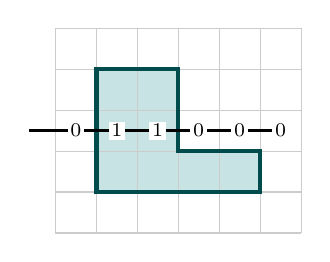
\begin{tikzpicture}[scale=.52]
\fill[teal!22] (1,1)--(5,1)--(5,2)--(3,2)--(3,4)--(1,4)--cycle;
\draw[step=1,gray!40,thin] (0,0) grid (6,5);
\draw[teal!60!black,line width=1.6pt] (1,1)--(5,1)--(5,2)--(3,2)--(3,4)--(1,4)--cycle;
\draw[->,thick] (-.65,2.5)--(5.7,2.5);
\foreach \x/\b in {0.5/0,1.5/1,2.5/1,3.5/0,4.5/0,5.5/0}
  \node[fill=white,inner sep=1pt] at (\x,2.5) {\scriptsize $\b$};
\end{tikzpicture}

{\small The scan toggles at each vertical polygon edge. A horizontal edge is\par
 accounted for by the parity equations in the two adjacent rows.}
\end{center}

\paragraph{Coordinate and arithmetic scope.}
Scaling by a common positive denominator and subdividing proves the same statements for simple rational rectilinear polygons. The number of grid cells can be large in the bit length of the coordinates but is primitive recursive in their numerical codes. The longest searches above may instead enumerate paths of length at most the number of graph vertices, with codes bounded by $(2+ab+a+b)^{2(ab+a+b+3)}$ for the dual walks. The row invariant in Lemma~\ref{lem:gridfill} is an equation of prefix parity bits. The assertion that all forest paths of length at most $V$ have the claimed cancellation is a bounded test. These are permissible induction formulas after Boolean compilation. Arbitrary Jordan embeddings require different separation information.

\begin{corollary}[The circle separates the plane]\label{cor:circlePlane}\label{idx-plane61}
For points equipped with positive distance from the unit circle, its complement in the presented plane has exactly two path components, the inside and the outside. Each point of the circle is in the boundary of both.
\end{corollary}
\begin{proof}
For the square $\|x\|_\infty=1$, a positive gap permits deciding the sign of $\|x\|_\infty-1$ from one sufficiently fine reading. The inside is convex, so contracts by straight segments. For two outside points choose a rational $R$ larger than both norms. Travel out each ray to the boundary of the square of radius $R$ and join the endpoints along that square. The latter path exists constructively by its perimeter parametrization: take a rational lift near each endpoint and interpolate in the covering line (use a radius-$1/4$ local chart to lift each named endpoint). Along the whole route the norm is at least the smaller original norm. No uniformly presented path with positive uniform clearance can join the two signs, since its norm along the path would take values arbitrarily close to $1$ by the approximate intermediate value theorem. The same holds when a pointwise positive clearance with a PR local test for the two signs is supplied, by the local connectedness test in Section~\ref{sec:metric-names}: signs restrict to an extensional locally constant bit on the parameter interval when a sign evaluator is supplied. For each square boundary point $p$, the points $(1\pm 2^{-j})p$, $j\ge1$, approach from the two sides. The explicit radial transformations in Section~\ref{sec:metric-names} are defined on the full plane, carry the square boundary to the unit circle, and carry each of the two strict norm inequalities to the corresponding Euclidean one. Their Lipschitz bounds transport positive clearance, giving the conclusion in the indicated path presentations.
\end{proof}

\section{Loops on a sphere and on a torus}\label{sec:loop}
A torus carries a loop that goes around its first circle once. On a two-dimensional sphere, every uniformly presented loop can be contracted. Both assertions have finite arithmetic proofs. Together they distinguish the two surfaces even when the hypothetical maps are given by evaluators and need not be simplicial.

\subsection{Counting turns by rational differences}
Write $C=\mathbb R/\mathbb Z$ using the dense rational presentation $\mathbb Q/\mathbb Z$. At rational inputs set
$d_C(x,y)=\min(|x-y|,1-|x-y|)$ for representatives in $[0,1)$. Completion uses the metric conventions of Section~\ref{sec:metric-names}. A loop is a uniformly presented map on $[0,1]$ with equal endpoint names. A free homotopy of loops is a uniformly presented map on the parameter square with equal values on the two vertical sides at each height. Boundary equalities are equalities to every accuracy. The unit loop is $t\mapsto t\bmod 1$.

A perimeter parameter identifies $C$ with the boundary of $[0,1]^2$: traverse its four unit edges at constant speed four, starting at the lower left corner. This map is $4$-Lipschitz into the sup metric. For the inverse, two points on the same edge are joined there. On adjacent edges the route through their common corner has length at most twice their sup distance. On opposite edges that distance is one and a shorter boundary route has length at most two. Dividing the length by four bounds their circular distance. The rational maps are inverses, and these bounds extend them to names, including corners. The radial homeomorphism in the metric section identifies this square with the round circle after centering and rescaling. Thus $C^2$ (here the Cartesian square of the circle) gives the usual product presentation of the torus.

\begin{lemma}[A winding obstruction]\label{lem:winding}\label{idx-surfaces10}
The unit loop in $C$ admits no uniformly presented free contraction.
\end{lemma}
\begin{proof}
Suppose a contraction is given. From its square-uniform modulus choose a square mesh $1/N$ such that adjacent true images differ by at most $1/16$, with $N\ge 16$. At each mesh point use one rational circle reading accurate to $1/32$. On the right repeat the left reading. On the bottom use $i/N\bmod 1$ exactly. On the top repeat one reading of the constant endpoint. All replacements are still accurate to $1/32$, by the side and endpoint contracts. Along every oriented mesh edge $pq$ there is a unique rational difference $\delta(p,q)$ congruent modulo one to $q-p$ and of absolute value $<1/4$: the circular distance of its readings is at most $1/8$. Compute it by testing three lifts, with at most one admissible. Reversing an edge negates its difference. The sum around a cell is an integer because the differences telescope modulo one. Its absolute value is $<1$, so it vanishes. Sum over all cells. Interior edges cancel and the left and right sums cancel because the readings coincide. The bottom sum in the positive horizontal direction is $N(1/N)=1$, including the wrap across zero. The top sum is zero. This contradicts the equality of the two sums.
\end{proof}

\paragraph{Other degrees.}
For the loop $t\mapsto kt\bmod 1$ with $k\in\mathbb Z$, take $N>8(1+|k|)$ in this argument. Each bottom difference is $k/N$, even at a wrap. Any two such loops joined by a uniformly presented free homotopy consequently have equal degrees. Conversely equal integers give the same loop. More generally every uniformly presented loop is freely homotopic to one of these, with a computable degree. Sample rational circle readings $r_i$ at mesh vertices with repeat at the seam, choosing mesh oscillation and reading error at most $1/32$ each. Lift $r_0$ to $a_0\in[0,1)$ and cumulatively add the short edge differences to get $a_i$. Then $k=a_N-a_0\in\mathbb Z$. Interpolate the $a_i$ linearly to $A(t)$. Throughout each mesh interval the circular distance from $A(t)\bmod1$ to the original loop is at most $3/32+2/32<1/4$. Two such close points have a unique signed short displacement. It is evaluated on names by approximating to any demanded accuracy and reducing their difference to the nearest lift; the strict $1/4$ margin avoids ambiguity at a half-integer. Multiplying that displacement by the homotopy parameter joins the two loops. Next interpolate linearly in the covering line from $A(t)$ to $kt$, then reduce modulo one. At $t=1$ both lifts differ from their values at $t=0$ by $k$, so this is a free homotopy throughout. For loops based at $0$, use the exact first and last readings $0$, with $a_0=0$. The same construction fixes the basepoint. For concatenated loops concatenate the polygonal lifts, translating the second to start at the endpoint of the first. Endpoint differences add. Reversal negates the difference. This proves $\pi_1(C,0)\cong\mathbb Z$ in this presentation. Coordinate projection and pairing of the homotopies give $\pi_1(C^r,0)\cong\mathbb Z^r$ for each finite $r$, including $r=0$.

\subsection{Choosing a cone point by a bounded scan}
For $d\ge3$ let $S_\infty^{d-1}$ be the boundary of $[-1,1]^d$. Write $\rho(u)=u/\|u\|_\infty$ when a positive lower bound on the denominator is available.
\begin{theorem}[Contraction on the cube boundary]\label{thm:loopSphere}\label{idx-surfaces22}
Every uniformly presented loop on $S_\infty^{d-1}$, $d\ge3$, has a uniformly presented free contraction, primitive recursive from its fixed evaluation and modulus routines. For based loops a contraction fixing the basepoint can also be produced.
\end{theorem}
\begin{proof}
Choose $m$ so the oscillation of $\gamma$ on a mesh interval is at most $1/16$. Read rational vertices $p_i$ within $1/16$ of $\gamma(i/m)$, repeating $p_0$ at $i=m$. They may be chosen on the cube boundary; the argument also works for readings in the ambient cube with the indicated error. For the polygonal interpolant $P$, each endpoint of its edge is within $1/8$ of the true value at any point of that interval. The convexity of the sup ball gives $\|P(t)-\gamma(t)\|_\infty\le1/8$. Thus $\rho((1-s)\gamma(t)+sP(t))$ joins $\gamma$ to $\rho(P)$ with denominator at least $7/8$.

For each of the $m$ edges find a nonzero rational covector $n_i$ perpendicular to both endpoints, supported on the first three coordinates. Take the cross product of the first three coordinates; if it vanishes, choose a coordinate vector perpendicularized by crossing it with a nonzero one of the two triples. If both triples vanish, use $(1,0,0)$. Exact rational equality decides all branches. For an integer $j$ put $u(j)=(1,j,j^2,0,\dots,0)$. The nonzero polynomial $n_i\cdot u(j)$ has at most two distinct integer roots: subtract two root equations, factor the nonzero differences, and a third root would force all three coefficients to vanish. Hence some $0\le j\le 2m$ avoids the roots for every edge. Set $w=u(j)/\|u(j)\|_\infty$ for the first such $j$.

The second homotopy is $\rho((1-s)P(t)+sw)$. Here is an explicit denominator bound on edge $i$. For $s\le1/8$, $\|P(t)\|_\infty\ge7/8$ and
\[
 \|(1-s)P(t)+sw\|_\infty\ \ge (7/8)(7/8)-1/8>1/2.
\]
For $s\ge1/8$, pair with $n_i$. The pairing with $P$ vanishes, giving the lower bound $|n_i\cdot w|/(8\|n_i\|_1)$. The minimum of these finitely many positive rationals and $1/2$ is an explicit positive $b$. The bound extends to all real parameters by rational approximation, with no decision about a real comparison required. On vectors of norm at least $b$, radial normalization is $(2/b)$-Lipschitz: subtract $u/\|u\|-v/\|u\|$, then bound the remaining term by $|\|v\|-\|u\||/\|u\|$. The polygon has a computable Lipschitz bound $m\max_i\|p_{i+1}-p_i\|_\infty$; ordinary product and sum estimates now give moduli for both homotopies. They agree at the join, and all stages are periodic in $t$.

For clarity, an explicit conversion to a based homotopy uses the track $h(s)=H(0,s)$ of the free contraction. At stage $s$ traverse $h|_{[0,s]}$, the loop $H(-,s)$, and the reverse of that track, on three equal parameter intervals. At $s=0$ shorten the two constant waiting intervals by a linear change of the time parameter to recover the original loop. At $s=1$ the middle loop is constant. Retract the outgoing and returning parts simultaneously by replacing their final track parameter $1$ by $1-s$, with a constant middle third at $h(1-s)$. This fixes both endpoints and terminates at the constant base loop. Every reparameterization has a rational piecewise formula and a modulus from the input.
\end{proof}

\begin{corollary}[Sphere and torus]\label{cor:sphereTorus}\label{idx-surfaces39}
The presented sphere $S^n$, $n\ge2$, has trivial based fundamental group. It is not uniformly presented homotopy equivalent to the torus $C^2$. In particular there is no homeomorphism with equipped uniform evaluators in both directions. The same distinction applies to $C^r$ for $r\ge1$.
\end{corollary}
\begin{proof}
Use radial normalization between round and cubical boundaries. If $f:C^r\to S^n$ and $g:S^n\to C^r$ had $gf$ uniformly homotopic to the identity, apply the sphere contraction to $f$ of the loop $(t,0,\dots,0)$. Compose it with $g$, attach the given homotopy at the first end, then project to the first circle. The result would contract the unit loop, contradicting Lemma~\ref{lem:winding}. The proof needs only this one composite homotopy.
\end{proof}

\paragraph{First-order interpretation.}
A construction yielding a homotopy is a recipe for PR evaluation and modulus \emph{terms} given fixed terms for the input. In the winding argument take parameters coding just the polygon, the endpoint witnesses and the rational grid for the allegedly contracting map. The test on every face is a bounded scan. Its conclusion is an equality of integer numerators after a denominator product. For the sphere contraction the exceptional value search has exactly $2m+1$ candidates; the count follows by summing the bit for each pair $(i,j)$ in either order. Bounds on $1/b$ are computable from the obtained positive rational. This explains why the proof can choose a pole depending on the loop without any principle selecting a point outside an arbitrary countable set.

\subsection{Lower homotopy groups of spheres}

The same choice of a direction avoiding finitely many linear subspaces
contracts a family of loops with several parameters. Use the based
cubical description: a representative in degree $k\ge1$ is a uniformly
presented map on $I^k=[-1,1]^k$ whose restriction to the boundary is one
specified named point $a$. Homotopies relative to the boundary have value
$a$ there at every time.

\begin{theorem}[Vanishing below the dimension of the sphere]\label{idx-higher10}
For $1\le k<n$, every such representative on the cubical sphere
$S^n_\infty=\{x\in[-1,1]^{n+1}:\|x\|_\infty=1\}$ has a uniformly
presented nullhomotopy relative to its boundary. Hence
$\pi_k(S^n,a)=0$ for these representatives, also in the round-sphere
presentation. Every two presented points of $S^n$ with $n\ge1$ can be
joined by a uniformly presented path. The constructions use primitive
recursion in the dimensions, mesh size and rational data, for each fixed
input evaluator and modulus.
\end{theorem}
\begin{proof}
Write $f$ for the input map, with a modulus $\mu$ on names in the maximum
metric. Take $m=2^{\mu(5)+1}$ and subdivide each parameter axis into $m$
pieces of length $l=2/m$. Two points of a mesh cube have images within
$1/32$. At each grid vertex $v$ take a rational vector $p_v$ within $1/32$
of $f(v)$, clipping to $[-1,1]^{n+1}$ if necessary. On \emph{every}
boundary vertex use the same reading of $a$. This makes the subsequent
polygonal approximation exactly constant on each boundary face, including
where different faces meet.

Here are the triangulation and its estimates. Within each grid cube write
the local coordinates as $t_i\in[0,1]$. Sort them as
$t_{i_1}\ge\cdots\ge t_{i_k}$, breaking ties by label. The simplex
vertices $v_0,\ldots,v_k$ start at the lower corner and successively
increase coordinates $i_1,\ldots,i_k$ by one grid step. For the affine
interpolant $P$ take the corresponding convex combination of the $p_{v_j}$
with weights
\[
 1-t_{i_1},\quad t_{i_1}-t_{i_2},\quad\ldots,\quad
 t_{i_{k-1}}-t_{i_k},\quad t_{i_k}.
\]
Exchanging equal coordinates changes only a zero-weight intermediate
vertex. On a shared cube face the vertices off the face have weight zero,
and the remaining coordinates have the same sorted order on either side.
The formulas consequently agree on all overlaps. On any one simplex,
$P=p_{v_0}+\sum_{j=1}^k t_{i_j}(p_{v_j}-p_{v_{j-1}})$, so its
Lipschitz constant is at most $2k/l=km$. This bound is global: for a
rational segment, split it where it crosses the finitely many grid and
coordinate-order hyperplanes. An equation holding on the entire segment
requires no cut. The maximum-norm lengths of successive subsegments sum
to the original length since all run along the same segment. This proves
the rational bound, whence extension gives a PR evaluator on names.
There are $M=m^k k!$ simplices in the enumeration (grid indices and
permutations). At rational parameters each vertex value used differs from
$f$ at the parameter by at most $1/16$; convexity and approximation give
$\|P-f\|_\infty\le1/16$ throughout. The first homotopy
$\rho((1-s)f+sP)$ has denominator at least $15/16$. At boundary
parameters its value depends only on $s$.

The $k+1$ rational vertex readings of each simplex admit a common
annihilating nonzero rational covector $c$ supported on the first $k+2$
coordinates. Indeed there are $k+1$ homogeneous row equations and $k+2$
unknowns. Row reduction uses at most $k+1$ pivots; choose a free coordinate,
set it to $1$ and the other free coordinates to zero, then back-substitute.
For $j\ge0$ put $u(j)=(1,j,\ldots,j^{k+1},0,\ldots,0)$ in
$\mathbb Q^{n+1}$. Each polynomial $c\cdot u(j)$ is nonzero as a
polynomial and excludes at most $k+1$ candidate integers. Indeed division
at a root $r$ gives the factor $T-r$ by coefficient subtraction. Every
other distinct root remains a root of the quotient. Repeating this on a
list of distinct roots more numerous than the degree would give a root of
a nonzero constant. The proof just uses rational operations on finite
lists. In the table counting excluded pairs (simplex, candidate), the
total therefore is at most $(k+1)M$. At least one of
$0,\ldots,(k+1)M$ has no exclusion. For its first such $j$ put
$w=u(j)/\|u(j)\|_\infty$. Its norm is one.

The second homotopy is $\rho((1-s)P+sw)$. For $s\le1/8$ the
denominator exceeds $1/2$ by $\|P\|_\infty\ge15/16$. On a simplex with
covector $c$ and $s\ge1/8$, pairing with $c$ gives the lower bound
$|c\cdot w|/(8\|c\|_1)$ because $c\cdot P=0$. Thus the minimum $b$ of
$1/2$ and these $M$ positive rational bounds works globally. The
inequalities follow first on rational parameters and then on names.
Normalization with this denominator is $(2/b)$-Lipschitz, as in the loop
proof. In both homotopies a convex mixture of two bounded vectors changes
by at most the larger endpoint displacement plus twice the change of the
time parameter. This estimate, $km$, the supplied modulus and $2/b$
give a modulus for the concatenated homotopy $H$. At the time seam use
target error $2^{-p-1}$ per side and double the time scale. The boundary
track $h(s)=H(v,s)$ is common to all $v\in\partial I^k$, with
$h(0)=a$ and $h(1)=w$.

We now keep the boundary fixed. Put $r=\|u\|_\infty$ for a parameter
$u\in I^k$. First deform $f(u)$ to its compressed copy using
$f(u/\max(r,1-s/2))$. The denominator is at least $1/2$, and at $r=1$
the input stays on the boundary. Next, at time $s$, use
\[
 \begin{cases}
  H(2u,s),&r\le1/2,\\
  h(2s(1-r)),&r\ge1/2.
 \end{cases}
\]
At the seam the values agree because $2u$ is a boundary point there.
At time zero this is the compressed copy, and at $r=1$ it equals $a$.
At time one the formula is $h(\min(1,2(1-r)))$ everywhere. Contract
it to $a$ with $h((1-s)\min(1,2(1-r)))$. The formula with cases is
evaluated first on rational parameters. The inputs to $H,h$ on the two
pieces vary by at most four times the domain displacement, and a segment
with one endpoint on either side can be split at its rational intersection
with $r=1/2$. Thus a common precision request on the two pieces, tightened
by one output bit and two input bits, yields a global modulus. The
case-free initial and final formulas have bounded denominators and
Lipschitz reparameterizations. Extension gives the three homotopies on
names, and their concatenation is relative to the boundary. The radial
homeomorphism transports the result to the round sphere.

For path connectedness take the two specified points as separate vertices,
with one rational reading close to each. Apply the same argument to these
two zero-dimensional simplices: a covector in the first two coordinates
for each single reading excludes at most one integer, so one of $0,1,2$
works for both. The two normalized interpolations join each original
point to the same $w$; reverse the second path to reach the second point.
\end{proof}

For Lean the new finite indices are a base-$m$ tuple and a permutation of
$k$ coordinate labels. Permutations may be obtained by filtering the
length-$k$ tuples with entries below $k$ for absence of repeats; for a simple
upper bound the search may use $m^k k^k$ in place of $M$ when $k\ge1$.
Prove the interpolation formula over rational inputs and its agreement
at ties before extending it. For the root bound keep a list of the distinct
roots already removed and the remaining coefficient vector; each synthetic
division shortens that vector by one and preserves vanishing at each of the
remaining listed roots. This is a bounded table invariant. The input for
the avoidance scan is the matrix of covectors and its output is the index
$j$ together with the rational $b$. These data supply all precision
requests in the three final homotopies.

\section{The boundary and twist of a Möbius band}\label{sec:ribbon}
Take $m\ge3$ unit rectangles indexed cyclically. Use coordinates $(x,y)$, $0\le x\le1$, $-1\le y\le1$. Glue the right end of panel $i$ to the left of panel $i+1$ by $y\mapsto e_i y$ with signs $e_i\in\{1,-1\}$. Put $e=\prod_{i<m}e_i$. Arithmetic on panel coordinates and all gluings is rational; maps agreeing on a seam specify maps on this finite presentation. Interior points have rectangular charts; at a seam use $x-1$ in the preceding panel and $x$ in the next, reversing the transverse coordinate when required. Horizontal-edge charts are half rectangles. These explicit charts also define the orientation and boundary used here.

\begin{theorem}[Parity of the twist]\label{idx-ribbon4}
Up to a panelwise affine homeomorphism there are two standard gluings, the cylinder for $e=1$ and the Möbius band for $e=-1$. The first has two boundary cycles and admits an orientation. The second has one boundary cycle and reverses a transverse direction around its core.
\end{theorem}
\begin{proof}
Replace the $i$th transverse coordinate by $p_i y$, with $p_0=1$ and $p_{i+1}=p_i e_i$ up to the last seam. All gluings except the last become the identity; the last has sign $e$. This coordinate change is its own inverse panel by panel. The horizontal edges are exactly the boundary in the displayed half-rectangle atlas. Travelling with increasing panel coordinate takes an edge sign $s$ to $e_i s$ at seam $i$. After $m$ steps the sign is $es$. If $e=1$ the two signs give separate cycles of length $m$; if $e=-1$ one cycle goes twice around, length $2m$. The same transition has Jacobian sign $e_i$ in the two-dimensional chart (the longitudinal coordinate increases on both sides). Consistent orientation signs $o_i$ satisfy $o_{i+1}=e_i o_i$, and exist exactly for $e=1$. Each panel interior is connected, so a locally constant orientation sign there is constant; the obstruction cannot be removed by subdividing a chart. In the product coordinates of the ambient interval bundle the calculation is also the reversal of any chosen normal direction to the central curve \emph{within the strip}.
\end{proof}

\begin{proposition}[Core circle, cut, and double cover]\label{idx-ribbon11}
Both bands strongly deformation retract to a circle. Cutting the Möbius band along its core gives one cylinder. Going twice round the base gives a cylinder double covering the Möbius band.
\end{proposition}
\begin{proof}
The maps $(x,y)\mapsto(x,(1-t)y)$ respect all signed seams, fix the core pointwise, and at $t=1$ take the band to it. The core is a cyclic interval of length $m$ with its endpoints glued. The displayed homotopy is given by rational multiplication on each panel with an explicit local Lipschitz bound. To cut, split each panel into two closed half panels and keep the two copies of $y=0$ distinct. Label such a half by $s=\pm1$ and use transverse coordinate $u=|y|\in[0,1]$. The gluing changes $s$ to $e_i s$ and preserves $u$; the length-$2m$ boundary permutation just calculated shows that the result is a single circle of $2m$ intervals times $[0,1]$. For the double cover, instead take $2m$ full panels with signs repeated. The product around the lifted base is $e^2=1$, so the resulting band is a cylinder. Reduction of the panel index modulo $m$ covers each small panel-interior chart and each seam chart by exactly two disjoint copies, sent homeomorphically onto it. The finite chart calculations give a two-sheeted covering map.
\end{proof}

Gluing two copies of the Möbius band along their boundary gives Euler characteristic zero in the polygonal cell count: each band has $2m$ boundary edges, $m$ vertical edges, $2m$ vertices and $m$ faces, and the common boundary has $2m$ vertices and $2m$ edges. This also illustrates directly why having the homotopy type of a circle determines neither the boundary count nor orientability of these bands.

\subsection{The circle is a one-manifold; the figure eight has a branch point}
Each point $c$ of the circle $C=\mathbb R/\mathbb Z$ has an arc chart. Choose a rational center $a$ within $1/16$ of $c$ and take signed differences from $a$ on the ball $d_C(a,x)<1/4$. These are unique lifts in $(-1/4,1/4)$ and have the inverse $t\mapsto a+t\bmod1$. Both maps have local Lipschitz bounds, and this arc contains $c$. The line itself has interval charts by translation. Consider instead the graph obtained by joining two unit-circumference circles at their basepoints, with shortest-path metric. The open ball of radius $1/8$ at the joint $o$ has four arms. For points on distinct arms in this ball, their distance is the sum of their distances to $o$: a route going the other way around a unit circle is longer than $1/2$.

\begin{proposition}[Branch obstruction]\label{idx-ribbon23}
The joint has no equipped interval chart. More generally a metric star with three or more arms at a vertex has the same obstruction. Here a chart contains a specified ball about the vertex, has both inverse identities, and supplies continuity at prescribed points and uniform moduli on the small closed arm segments used in the proof.
\end{proposition}
\begin{proof}
Suppose $f$ is such a chart with inverse $g$, with $b=f(o)$. Take three equal short closed arm segments $[o,p_i]$ of positive rational length $l$, inside the chart and the $1/8$ ball in the example. Write $b_i=f(p_i)$. The continuity bound for $g$ at $b$ for target error $l/2$ gives a positive threshold below which $b_i$ cannot lie from $b$, since $g(b_i)=p_i$. Consequently one can decide on which side of $b$ each $b_i$ lies using rational readings at precision finer than a quarter of this threshold. Two lie on one side. Choose a rational $c$ strictly between $b$ and both these endpoint values, with all three inequalities witnessed by positive margins. It lies in the interval chart.

Write $z=g(c)$. On either of the two arms the approximate intermediate value theorem in Section~\ref{sec:metric-names} gives points with images arbitrarily close to $c$. It applies to named endpoint values by choosing readings accurate within the strict margins (reverse signs on decreasing arms). Applying the continuity modulus of $g$ at $c$ gives arm points at distance at most $2^{-k}$ from $z$ on each arm, for any given $k$. These two points are at most $2^{1-k}$ apart; their distance equals the sum of their distances from $o$. Thus $z$ is within $3\cdot2^{-k}$ of $o$ for all $k$, so $z=o$. Applying $f$ gives $c=b$, contradicting the chosen margin. This argument explains the failure at the joint without assuming the existence of an exact zero for a general intermediate-value problem.
\end{proof}

\subsection{A solid handle and an embedded torus}
The cup-and-doughnut example requires specifying which surface one means. The following model includes the interior of the vessel's wall as solid material, and takes its complete boundary, including the inner bowl, as the surface.

\begin{proposition}[A handled ball and its boundary]\label{idx-ribbon35}
Let $D=[-1,1]^2$. A ball presented as $[0,1]\times D$, together with a second copy of $[0,1]\times D$ attached by its end disks to the two end disks of the ball with matching transverse coordinates, is a solid torus. Its boundary is $C\times C$, and both admit explicit embeddings in three-space.
\end{proposition}
\begin{proof}
Orient the two longitudinal intervals consecutively. Their endpoint gluings make a circle of length two, and leave the $D$ coordinate unchanged. The quotient is thus exactly $C\times D$ by the piecewise rescaling that sends each interval to half a turn. The disk interiors at the attachments are interior points after gluing by a product chart. The remaining lateral faces and their seams form $C\times\partial D$, identified with $C\times C$ by the perimeter parameter. This also supplies the boundary charts at the former rims.

Here is an embedding with an explicit inverse. For $u=(u_1,u_2)\in\partial D$ and $v=(v_1,v_2)\in D$, put
\[
      (X,Y,Z)=((3+v_1)u_1,(3+v_1)u_2,v_2).
\]
Writing $t=\max(|X|,|Y|)$ gives $t=3+v_1\ge2$. Recover $u=(X/t,Y/t)$ and $v=(t-3,Z)$. Thus the image is given by $\max(|t-3|,|Z|)\le1$ and its boundary by equality. All operations give PR evaluators with uniform bounds on this bounded region. For example coordinatewise multiplication on these parameter ranges changes by at most five times the sup displacement, and division uses $t\ge2$.

A hollow-looking bowl can be made in the ball before attaching the handle. With $u\in D$ and $s\in[0,1]$, put $h(u)=(1+\|u\|_\infty)/2$. The map $(s,u)\mapsto(u,s h(u))$ produces material between a flat bottom and a top surface depressed at its center, with the rim at height one. Its inverse uses division by $h\ge1/2$. Mark the images of the two attaching disks (or transport a chosen pair by a supplied ball chart); postcomposing that chart simply transports the gluing. This establishes the advertised cup comparison for a ball with one ordinary solid handle, without needing a recognition theorem for physical objects.
\end{proof}

\section{Why subgroups of free groups are free}\label{sec:schreier}
The overview gives this consequence as an example of topology proving a theorem of algebra. The topology here is a graph covering a bouquet of circles. Even when that graph is infinite, the part seen by a word can be computed within a bound set by the word itself.

\begin{theorem}[Schreier basis for a presented subgroup]\label{thm:schreier}\label{idx-schreier4}
Fix the free group $F_r$ of reduced words on $r$ letters and their inverses. For each fixed PR membership test $H(w)$ satisfying the subgroup and reduction laws, there is a PR test for basis symbols and mutually inverse PR procedures between elements of $H$ and reduced words on those symbols. In particular the subgroup is freely generated by a specified, possibly infinite, decidable set of words.
\end{theorem}
\begin{proof}
Use right cosets $Hw$ as notation for the numerical equivalence relation
$u\sim v$ if $uv^{-1}\in H$. Products always include free reduction. The subgroup laws give equivalence, and appending the same word preserves it. Among reduced $v\sim w$ with $|v|\le |w|$, choose the shortest, breaking ties lexicographically in a fixed order on signed letters. Call it $R(w)$. This is the least of the whole class because $w$ itself is a candidate. In particular $R$ is constant on classes. A scan of at most $(2r+1)^{|w|+1}$ candidates suffices (for $r=0$ only the empty word occurs).

Every prefix of a representative is again a representative. Otherwise replace that prefix by a smaller equivalent word and append the unchanged suffix. Free reduction can shorten it; if its length stays equal, the first lexical improvement persists. The result represents the same class and is smaller, a contradiction. The representatives therefore form a rooted tree under deleting the last letter, with root the empty word. Consider the graph with vertices these representatives and one oriented edge $(u,a)$ from $u$ to $v=R(ua)$ for each positive generator $a$. Traversing that edge backwards reads $a^{-1}$. The prefix tree consists exactly of edges for which $ua=v$ as reduced words: if cancellation occurs, the endpoint is the prefix of $u$; without cancellation, $u$ is the prefix of $v$. Each non-tree edge gives the basis symbol $(u,a)$ with value
\[
                          b(u,a)=uav^{-1}\in H .
\]
The test for a symbol is $R(u)=u$, $1\le a\le r$, and $ua\ne R(ua)$ as reduced words.

For a subgroup word $h$, start at the root and read it letter by letter. At a positive letter use the indicated edge; at $a^{-1}$ its positively oriented edge starts at $R(ua^{-1})$. Record nothing on tree edges and the signed symbol on every other edge; freely reduce this output. The final vertex is the root. A letter followed by its inverse traverses an edge and immediately returns on it, so removing this pair leaves the reduced output invariant. Two subgroup words concatenate as two loops at the root. Thus the reading map is a homomorphism. In the reverse direction substitute $b(u,a)$ for its symbol, using inverses when appropriate. The substituted word of a walk from $u_0$ to $u_k$ equals $u_0\,w\,u_k^{-1}$, since the factors at intermediate vertices cancel, and the omitted tree factors equal the identity. For a based loop this gives $h$ back. Conversely the path reading $b(u,a)$ follows the tree out along $u$, traverses the indicated non-tree edge and follows the tree home along $v^{-1}$. It records that one symbol. This proves mutual inverseness, generation and freedom. Distinct symbols have distinct group elements, since reading their expansions recovers the symbols.

At step $j$ of reading an input of length $L$ the representative has length at most $j$. The difference between testing a coset and deciding a real or infinitary predicate is important here: $H$ is a supplied numerical term. The proof of the reading identities is induction along a bounded word with tests on finite strings. It proves an iPRA schema with the stated membership and subgroup hypotheses.
\end{proof}

\begin{corollary}[The finite-index rank formula]\label{idx-schreier22}
Given a transitive right action of $F_r$ on $d\ge1$ numbered points by $r$ permutation tables, the stabilizer of a specified point is free of rank $1+d(r-1)$.
\end{corollary}
\begin{proof}
Send $Hw$ to the image of the basepoint under $w$. The test $uw^{-1}\in H$ says precisely that $u$ and $w$ send the basepoint to the same point. Transitivity gives every target and elementary path search gives a word of length at most $d-1$ reaching it. The graph has $d$ vertices and $dr$ positive edges, including loops and parallel edges. Its prefix spanning tree has $d-1$ edges; the remaining $dr-d+1$ give the displayed rank. When $r=0$, transitivity forces $d=1$ and the formula gives zero.
\end{proof}

\begin{theorem}[A finite list of subgroup generators suffices]\label{thm:fold}\label{idx-schreier29}
Given a finite list of words in $F_r$, one can compute a finite labelled graph deciding membership in their subgroup and a finite free basis. The construction is uniform and PR in the whole list.
\end{theorem}
\begin{proof}
Make a base vertex and a subdivided loop for each nonempty word, with its successive directed edges labelled by the input letters. An edge has a formal reverse carrying the inverse label. The reduced labels of closed based walks form exactly the generated subgroup. Indeed, cancelling immediate edge reversals leaves the label unchanged in $F_r$, and away from the base a walk without reversals must continue around the current loop until it returns. Conversely, concatenating the given loops and their reversals realizes each product.

If two distinct oriented edges of the same label start at the same vertex, identify them, their reverses, and their terminal vertices. Scan and repeat. This operation preserves the subgroup read by based walks. A walk downstairs lifts edge by edge to the old graph with possible jumps between the two merged terminal vertices. Bridge each jump by going backward along one old edge and forward along the other. This contributes a freely trivial label. The same bridge at the beginning or end aligns the lifted basepoint. If the terminal vertices already coincide, no bridges are needed. Conversely, projecting an old walk preserves its label. Each fold removes at least one unoriented edge, so their number is bounded by the sum $L$ of input lengths.

In the final graph each signed label has at most one outgoing edge per vertex. A based walk labelled by a word with adjacent inverse letters traverses an edge and its actual reverse at that pair: uniqueness holds at the intermediate vertex. Hence a reduced word is in the subgroup exactly when its unique attempted walk exists and ends at the base. This is a PR membership test. Choose a spanning tree; for each non-tree edge choose one orientation, take the tree path out, that edge, and the tree path home. These loops freely generate the edge-path group by the same cancellation and reading argument as above. The map from this group to $F_r$ is injective: a walk without immediate reversals has a freely reduced label, by determinism at each vertex. A nonempty reduced loop therefore cannot have trivial label. The labels of the constructed loops give a finite free basis of the prescribed subgroup. Breadth-first parent computation, each conflict search and relabelling, and the $L$ fold iterations are bounded finite operations.
\end{proof}

\section{Colorings of knot diagrams}\label{sec:knotcolor}
The figure-eight knot pictured at the beginning of \emph{Topology} has
a four-crossing diagram. Can one turn this diagram into a circle by
moving its strands? A count with five colors answers the question.
A separate four-letter computation identifies the knot with its mirror.

\subsection{Local rules and Reidemeister moves}
Use a finite diagram with crossing records. Each crossing has four
half-edges in cyclic order, an opposite pair marked over, and the other
pair marked under. Edges pair the half-edges between crossings. Store
each crossing-free circle separately. For planar diagrams one may give a
planar drawing or a list of elementary tangle slices as well. An
$n$-coloring, $n\ge1$, assigns each edge (and each free circle) a residue
modulo $n$. At a crossing the two over colors agree, say with $y$, and the
two under colors $x,x'$ satisfy $x+x'=2y$. Thus the under color changes
by the operation $x*y=2y-x$. Following a strand across successive
overcrossings gives the equivalent familiar coloring of arcs between
undercrossings. Write $C_n(D)$ for the number of colorings.

\begin{theorem}[Fox coloring invariance]\label{idx-knots20}
A Reidemeister move induces a bijection on $n$-colorings fixing the
untouched part of the diagram. In particular $C_n$, and the existence of
a nonconstant coloring, are invariant under a finite sequence of
diagram moves, for every positive modulus.
\end{theorem}
\begin{proof}
In a type I kink the over color is also one of the under colors,
since the small loop directly joins the corresponding half-edges. The
crossing equation forces the other under color to agree. The local
extension is unique and has equal colors at both ends.
In type II one strand passes over twice with the same color $y$. A
color $x$ on the other strand changes first to $x*y$ and then back to
$x$, since $(x*y)*y=x$. This determines all internal colors uniquely.

For type III name the strands by their relative height. Read the top
color as $z$, the middle color on the side before it passes under the
top as $y$, and the bottom input as $x$. On one side of the move the
bottom passes under the middle and then the top, leaving with
$(x*y)*z$. On the other side it passes under the top and then under
the transformed middle, leaving with $(x*z)*(y*z)$. These agree since
both equal $x-2y+2z$. The top stays $z$ and the middle exits with $y*z$
on both sides. These three parameters determine all local colors, so
the two local assignments agree at every exterior port. Directions here
are choices for tracing the three strands. Reading a strand backwards
uses the same crossing relation because it is involutive. The argument
therefore also covers reversed and rotated local pictures. Gluing the
unchanged exterior identifies the full colorings even if some exterior
ports are joined to one another. Constant colorings extend constantly
in both directions. Relabeling the edges simply permutes color
coordinates. Composing the local bijections proves the assertion.
\end{proof}

\subsection{Two-strand links and the figure-eight}
A braid word is read from top to bottom, and its closure joins each bottom
position to the top position of the same index. For a positive crossing
with the left strand passing over the right, the pair of colors transforms
by
\[
 B(x,y)=(2x-y,x),\qquad B^{-1}(x,y)=(y,2y-x).
\]
All untouched positions keep their colors. Once the top colors are
given, all internal colors are forced, so the colorings of the closure
are exactly the fixed vectors of the braid word modulo $n$.

\begin{theorem}[Two-strand closure formula]\label{idx-knots65}
For the closure $D_m$ of the two-strand braid with signed exponent
$m\in\mathbb Z$,
\[
                  C_n(D_m)=n\gcd(n,|m|).
\]
For odd $m$ this is a knot, and for even $m$ it is a two-component link.
The positive odd exponents give pairwise distinct diagram classes.
\end{theorem}
\begin{proof}
Put $a=x-y$. Both crossings preserve this difference. The positive
crossing adds $a$ to both entries and its inverse subtracts $a$.
Iteration gives $B^m(x,y)=(x+ma,y+ma)$. The closure condition is thus
$ma=0$ modulo $n$. Set $h=\gcd(n,|m|)$ and $n'=n/h$.
The admissible residues are exactly $0,n',\ldots,(h-1)n'$.
Indeed, cancelling $h$ gives $n'\mid (m/h)a$, and B\'ezout's identity
for the coprime integers $n',m/h$ gives $n'\mid a$. The converse
follows by multiplication. The identity is obtained by the ordinary
Euclidean algorithm with decreasing remainders, carrying the two
coefficients in each division. For $m=0$ every residue works. There are
$n$ independent choices of $y$, giving the formula. Every crossing
transposes the two strand positions, so the cycles of the endpoint
permutation give the asserted component counts. If $1\le m<k$ are odd,
use $n=k$: $C_k(D_k)=k^2$ while $C_k(D_m)\le km<k^2$.
\end{proof}

The trefoil is the closure $D_3$ and has nine three-colorings, six
nonconstant. At modulus three the crossing equation says that the
three arc colors are all equal or all different, as checking $x=y$ or
$x\ne y$ shows. The crossing-free unknot has exactly three
three-colorings, one per constant color. Thus no finite Reidemeister
sequence takes one of these two diagrams to the other.

\begin{proposition}[The figure-eight diagram]\label{idx-knots98}
Write $a=\sigma_1,b=\sigma_2$ for the adjacent crossings of three
strands. The figure-eight diagram is the closure of $w=(ab^{-1})^2$.
It has $C_n(w)=n\gcd(n,5)$. Its diagram class is distinct from the
unknot and the trefoil. It is equivalent to its mirror and has
unknotting number one under diagram moves and crossing changes.
\end{proposition}
\begin{proof}
Apply $B$ on slots $1,2$, then $B^{-1}$ on slots $2,3$, twice.
For input $(x,y,z)$, put $u=x-y$, $v=y-z$. Subtracting the input from
the output gives $(3u+v,-u-2v,-4u-3v)$. Vanishing is equivalent to
$v=-3u$ and $5u=0$ modulo $n$. Given $z,u$, these equations reconstruct
all three input colors. Counting $u$ as in the previous proof gives the
formula. At $n=5$ the count is $25$, whereas the trefoil and unknot
both have $5$. At $n=3$ the figure-eight has only its constant colorings.

Mirroring across the projection plane changes all crossing signs, giving
$(a^{-1}b)^2$. The braid relation $aba=bab$ is a type III move. Thus
$\Delta=aba=bab$ satisfies $\Delta a=b\Delta$ and $\Delta b=a\Delta$ by
concatenation. Conjugation by $\Delta$ interchanges $a,b$, including
their inverses. Conjugation preserves a closed braid diagram class:
move the cut around the annular closure, which cyclically permutes the
word, then cancel inverse pairs by type II. Hence the mirror has the
class of $(b^{-1}a)^2$, which cyclically shifts to $w$.

Change the first $a$ in $w$ to $a^{-1}$. Cyclically shifting its last
letter to the front gives $b^{-1}a^{-1}b^{-1}a$. The inverse braid
relation changes the first three letters to $a^{-1}b^{-1}a^{-1}$, so
cancellation leaves $a^{-1}b^{-1}$. Its rightmost strand now takes
part in only its last crossing. On closure the strand and its outer
closing arc form an empty kink, removable by a type I move after
straightening that arc. The two-strand closure left over is $D_{-1}$,
again a single removable kink. One crossing change therefore suffices.
Zero cannot suffice by the count at modulus five.
\end{proof}

\subsection{Joining knots and the arithmetic statement}
For connected sums use diagrams cut into $(1,1)$-tangles, each drawn
with one input at the top and one output at the bottom. Closing the cut
by an exterior arc gives its original diagram. Stacking two tangles and
closing the result gives their marked connected sum. Represent a tangle
by successive horizontal slices containing one crossing, one birth of a
pair at a local minimum when read in the chosen direction, or one death
of a pair. These are combinatorial instructions about adjacent positions.

\begin{proposition}[Connected-sum count]\label{idx-knots143}
For two such presented knots,
\[
 n C_n(D_1\mathbin{\#}D_2)=C_n(D_1)\,C_n(D_2).
\]
In particular the connected sum of $s\ge1$ trefoils has $3^{s+1}$
three-colorings. Distinct positive values of $s$ give inequivalent
diagrams.
\end{proposition}
\begin{proof}
On a horizontal slice with colors $c_1,\ldots,c_k$ the alternating sum
$c_1-c_2+c_3-\cdots$ is conserved. A crossing preserves the difference
of the two entries it acts on. Inserting or removing an adjacent equal
pair contributes zero and changes no subsequent sign. At the two ends
there is only one entry, so every coloring has equal endpoint colors.
It extends uniquely across the closing arc. Translating all residues by
a constant preserves the equations and bijects the colorings at any two
specified endpoint colors. Thus for $D_i$ let $q_i$ be the number with
endpoint color zero. Its total is $nq_i$. For the stack, choose the
common endpoint color in $n$ ways and the two restricted colorings in
$q_1q_2$ ways. This gives the identity and, by induction from
$C_3(D_3)=9$, the claimed powers of three.
\end{proof}

For Lean, encode a crossing record by four edge indices and a bit for
the over pair. Define \texttt{colorOK} by one modular test and one
equality per crossing. With $e$ edge variables including free circles,
enumerate the $n^e$ vectors by radix digits (handle $n=1$ by the unique
zero vector). For each external port table the type I--III proofs give
explicit inverse functions between extension lists. Define
\texttt{braidStep} on indexed color lists, and prove by induction on
the word the fixed-vector test for the closure. Implement the signed
two-strand formula as two inductions on $|m|$. For the connected-sum
proof the induction predicate is equality of the current and initial
alternating sums, evaluated modulo $n$. Thus iPRA proves the invariant
for every coded move list, and unequal counts rule out any such list.
Classically Reidemeister's theorem connects this diagram equivalence to
ambient isotopy of tame knots. The iPRA claims above work directly with
diagrams and the displayed moves. A translation of arbitrary ambient
isotopies into move certificates would be a separate geometric theorem.

\section{Dimension, fixed points, and tangent fields}\label{sec:companions}
Three complete earlier ProveIt manuscripts are included with their editable sources. They address prominent instances where an approximation error or an inverse modulus changes the statement one can prove. They are credited continuations of this collection. Their results are excluded from the count of numbered results in the main manuscript.

\paragraph{Dimension cannot be compressed at every scale.}
In \path{companions/dimension_invariance_ipra/dimension_invariance.pdf}, the numerical input is an arbitrary rational table $F:\{0,\ldots,N\}^d\to\mathbb Q^m$, $d,N\ge1$, and a rational $h>0$. If $d>m$ there is either a pair on opposite coordinate faces whose images have sup distance $<h$, or a pair of vertices of one Kuhn simplex whose images have sup distance $\ge h/d$. Both alternatives exhibit their vertices. The proof pairs incident facets to obtain cubical Sperner parity and uses staggered target grids: distinct boundary positions tied to the same target coordinate are separated by at least $h/d$. Sampling an equipped map on a sufficiently fine cube excludes the second alternative. An inverse separation bound excludes the first for an embedding with the specified inverse control. Applying the argument in both directions gives equality of dimensions for the indicated homeomorphic Euclidean presentations. The finite dichotomy is stronger evidence for its arithmetic content than a contradiction obtained by assuming an undefined continuous injection. The full parity proof, offsets and inverse hypotheses are in that manuscript.

\paragraph{A near-fixed point of a simplex map.}
In \path{companions/approximate_brouwer_ipra/brouwer.pdf}, $A(x,s)$ reads a rational simplex point at rational $x\in\Delta^d$ and has the contract
\[
 s,t\ge m,\quad \|x-y\|_\infty\le2^{-\mu(m)}
   \quad\Longrightarrow\quad\|A(x,s)-A(y,t)\|_\infty\le2^{-m}.
\]
With $m=k+2$ and $N=2^{\max(m,\mu(m))}$ the proof finds a rational $x$ of denominator $N$ such that for every $s\ge m$,
\[
             \|x-A(x,s)\|_\infty\le\frac{d}{d+1}\,2^{-k}.
\]
A fully labelled simplex exists by a facet parity count on at most $N^d$ cells. The coordinate residuals sum to zero because both vectors have barycentric mass one. Combining the sign information from the colors with the oscillation bound gives the displayed estimate. The paper also gives the changes of domain for cubes and balls. Each precision has its own witness; an additional selection argument would be needed to get a single exact fixed point.

\paragraph{Hairy balls and the parity of the dimension.}
In \path{companions/hairy_ball_ipra/hairy_ball.pdf}, the input dimension is $n=2m$, $d=n+1$. Rational directions are parametrized by $\|p\|_1=1$, representing $p/\sqrt{p\cdot p}$ on the round sphere. The PR evaluator $A(p,h)$ satisfies a regularity bound $\|A(p,j)-A(p,h)\|_1\le2\,2^{-h}$ for $j\ge h$, a same-stage variation bound $3\,2^{-h}$ whenever the input distance is at most $2^{-\mu(h)}$, and $|p\cdot A(p,h)|\le2^{-h}$. For $t=k+6$ and $D=2d\,2^{\mu(t)}$, it finds a rational direction $q$ with $Dq\in\mathbb Z^d$ such that
\[
       \|A(q,t)\|_1\le\tfrac34\,2^{-k},\qquad
       \|A(q,j)\|_1\le\tfrac{25}{32}\,2^{-k}\quad(j\ge t).
\]
The signed fundamental chain of a cross-polytope distinguishes the identity from the antipodal map in even sphere dimension. If no observed vector were small, the corrected tangent data would produce successive compatible labels joining those two maps; the chain calculation forces a pair of opposite labels instead. The companion proves the mesh and sampling bounds and converts a direction into a rational unit-vector witness with prescribed error. Its sharpness section explains the difficulty of selecting exact zeros.

\begin{proposition}[The other parity]\label{prop:oddfield}\label{idx-companions27}
On every odd-dimensional round unit sphere there is an explicitly presented tangent vector field of constant Euclidean length one.
\end{proposition}
\begin{proof}
The ambient dimension is even. Pair the coordinates and define
$J(x_1,x_2,\dots)=(-x_2,x_1,\dots)$ with the same rotation on each pair. Each pair contributes $-x_1x_2+x_2x_1=0$ to the dot product with $x$. The two squares in a pair are exchanged, so $\|Jx\|_2^2=\|x\|_2^2=1$. A signed permutation is 1-Lipschitz; at each precision simply permute and negate the readings of the input. The identities transfer to names by error removal. On $S^0$, the tangent space is zero and the two base points are rational.
\end{proof}

\section{From the proofs to Lean derivations}\label{sec:formal}
The formalization target for a closed arithmetical claim $\varphi$ is a value of type $[\,]\vdash[\mathsf{PRAAx}]\,\varphi$ in ProveIt's ordinary system. For a schema, first fix the PR syntax of the evaluators; put their arithmetic contracts in the antecedent or context. A semantic Lean theorem about functions on \texttt{Nat} is a useful specification. To certify the strength of the theorem one must construct the indicated object-language derivation.

\subsection{Syntax, modules, and a worked target}
We used the following interfaces from the repository at commit
\href{https://github.com/VladimirReshetnikov/ProveIt/tree/6d03f3643ebb91a6243eb1e35e7599b388197786}{\texttt{6d03f3643e}}.
\texttt{ConciseIPRA.PR} defines \texttt{PR k} (zero, successor, projections, composition and primitive recursion), terms \texttt{PTm n} built by variable and application, and \texttt{PRAAx}. In \texttt{PR.prec} the recursion argument occurs first; the step arguments begin with the predecessor and old state. The formulas and derivations use \texttt{Fm} and \texttt{Prf}. \texttt{PRA.qfInd} takes the quantifier-free check and derivations for the base and step. The module \texttt{IPRADerivations.Foundations.GuardedTrace} supplies \texttt{guarded\_loop}, \texttt{guarded\_trace}, and versions extracting every stage. \texttt{IPRADerivations.Core.IntCertificates} supplies signed integer terms \texttt{ZT}, their equality formula, and the sound ring lifting operation \texttt{ZT.derive}. Use \texttt{pra\_iff\_native} in \texttt{ConciseIPRA.NativeBiInterpretation} once an ordinary derivation has been obtained.

\paragraph{The rectangular target from the circle argument.}
Encode horizontal rational increments on a $(w,h)$ grid by a row-major array $H$ with $w(h+1)$ entries. Encode the vertical ones by $V$ with $(w+1)h$ entries. Multiply by the product of the positive denominators, so both signed arrays use integers and a common positive scale $D$. Index $H$ by $(j,i)\mapsto jw+i$, $V$ by $(j,i)\mapsto j(w+1)+i$. Let $B(j,r)$ be the sum of the first $r$ horizontal entries of row $j$. The displayed formula is an actual target for numerical coding, with each bounded conjunction expanded as in Lemma~\ref{lem:bounded}:
\[
\begin{split}
 \operatorname{Valid}(H,V,w,h)\ \land\;
 &\bigwedge_{j<h,\ i<w}
 [H_{ji}+V_{j,i+1}=V_{ji}+H_{j+1,i}]\\[-2pt]
 {}\land\;&\bigwedge_{j<h}[V_{jw}=V_{j0}]
       \quad\Longrightarrow\quad B(0,w)=B(h,w).
\end{split}
\]
Here subscripts such as $V_{jw}$ mean row $j$, column $w$. The inner invariant at prefix $r$ is
\[
 B(j,r)+V_{j,r}=V_{j,0}+B(j+1,r).
\]
At zero it is an identity. Add the next cell equality and cancel the repeated vertical edge. At $r=w$ substitute seam equality. The outer invariant $B(0,w)=B(j,w)$ advances by transitivity. Both are quantifier-free equations after substituting the PR table-access and summation terms. This is the entire uniform telescope derivation, including the empty rectangle. To finish the circle theorem, add a stage selecting signed residues in $(-D/4,D/4)$ at each edge; its bounded flag records congruence to the difference of endpoint readings modulo $D$. A cell sum has absolute value $<D$ and is divisible by $D$, hence zero. On the bottom row take the common scale divisible also by $N$ so the total is $D$. On the constant top row it is zero. The side and sampling assumptions in Lemma~\ref{lem:winding} supply exactly those checks.

The new file \texttt{lean/GridWinding.lean} expresses both iterations for ordinary Lean integer arrays. \texttt{lean/ObjectGrid.lean} gives a candidate proof-producing version: for every external rectangle size and every array of symbolic \texttt{ZT} entries it combines object-level cell proofs and seam proofs into an object-level row equality. The last step for the \emph{uniform} numerical target is to replace the two external size inductions by the two object-level guarded loops just specified. These new files were not compiled in this build. The repository's reusable finite-topology, metric, algebraic and sphere modules are included unchanged in \texttt{companions/}; their upstream build status is recorded separately in the archive guide.

\subsection{Definitions and order of the remaining work}
The relevant definitions, bounds, and witness-producing invariant for each family occur together in the preceding proofs. The following is a dependency order for implementing them in the same object calculus. All functions can be made total by returning zero on malformed tables; validity always occurs in the antecedent.
\begin{enumerate}
\item \textbf{Arrays and arithmetic.} Define \texttt{bit}, \texttt{read}, \texttt{write}, \texttt{firstHit}, \texttt{allBelow}, prefix parity, and signed rational comparisons using the encoding in Section~\ref{sec:arithmetic}. Prove read-after-write at equal and unequal indices, the prefix fold equations, and the witness specifications of Lemma~\ref{lem:bounded}. For rational linear operations prove compatibility with scaling both numerators and denominators and enforce the denominator tests.
\item \textbf{Spaces and graphs.} \texttt{Open} tests upward closure over all $n^2$ pairs. \texttt{LeastNbr} intersects all open masks containing the given point. \texttt{Reach} repeats one mark expansion $n$ times, storing a parent at each new marked vertex. Prove that marks have recorded paths and that closure under adjacency holds at the end. The component, subcover, quotient and beat-point verifiers in the finite section use these three operations. For grid drawings define the two edge arrays, row parity and the dual adjacency test. The exact recurrences of Lemma~\ref{lem:gridfill} yield boundary after filling, and filling after boundary; the forest proof gives the face count.
\item \textbf{Chains and reduced words.} Define face size, simplex image and boundary by enumeration of one-vertex deletions. Pair the two deletion orders; each target bit then cancels in $d^2$. Carry a column and its preimage together in elimination. Extend this in the order specified at the end of Section~\ref{sec:algtop}; the projection matrices from interval splitting give the barcode. For the polygon models use the explicit signed substitutions, testing the free coordinates and the residue modulo two. For graph words use a signed-letter stack. Store the current representative and emitted symbols for Theorem~\ref{thm:schreier}. Its prefix invariant is that their expansion equals the scanned input prefix times the inverse of the representative. In folding, store the vertex equivalence and images of oriented edges; the two-edge bridges lift a given word with a bounded certificate at each fold. For Fox colorings the data and move bijections are the crossing records of Section~\ref{sec:knotcolor}.
\item \textbf{Cauchy names and charts.} For each fixed input array term put the universally quantified regularity and modulus formulas in the context. A new name is an actual PR term in the precision and all free parameters. To prove a comparison, fix all outer stage indices, derive a rational estimate with auxiliary error $C2^{-s}$ and remove that error as in the metric section. Implement grid rounding, clamped interval maps, rational square-root approximation, sign-certified division, and the local chart inverses there. Cantor coding adds finite binary prefixes, ternary interval endpoints and finite metric nets. Branch decisions on real names are implemented through finite readings with a proved positive margin, or by gluing uniformly compatible rational formulas.
\item \textbf{Higher homotopy and surfaces.} Implement \texttt{kuhnWeights}, deterministic rational elimination for a covector, root counting by polynomial division and the $j$-scan on the moment curve. The output certificate contains the successful $j$, all covectors and the rational lower bound $b$. Check annihilation and nonzero pairings by finite products before defining the normalized coning name. The collar formulas prove the boundary equations at every stage. For the Möbius atlas, store $m$ seam bits; the invariant for a lifted side after $i$ seams is $s\prod_{j<i}e_j$. The branch obstruction uses just three segment maps and the interval search, with no classification of general manifolds.
\end{enumerate}
\paragraph{What is checked.}
The archive provides runnable rational and finite regression checks for the principal combinatorial constructions. The supplied Lean code and declaration-level plan give a path to formal completion. The complete collection of uniform object-language derivations is still to be constructed. The bare theorem that a search routine is PR, a passing finite test, or an ordinary Lean proof in a stronger logic does not close that remaining step.

\section{Source map and scope}\label{sec:sources}
The starting text is the English Wikipedia article \href{https://en.wikipedia.org/wiki/Topology}{\emph{Topology}}, especially its motivation, surface table, general and algebraic topology sections, and applications to data. The table groups its assertions with topics on its immediate outgoing pages. Some statements are direct arithmetic versions of statements in those pages. Others are consequences or tools developed here to explain a linked topic.
\begingroup\small
\renewcommand{\arraystretch}{1.15}
\begin{longtable}{@{}L{.31\linewidth}L{.63\linewidth}@{}}
\toprule
Article topic or linked page & Proven scope in this collection\\
\midrule\endfirsthead
\toprule Article topic or linked page & Proven scope in this collection\\\midrule\endhead
\href{https://en.wikipedia.org/wiki/Topological_space}{Topological space}, open and closed sets & Section~\ref{sec:finite-spaces} reconstructs all finite topologies from preorders, solves separation and continuity tests, and reconstructs finite $T_0$ spaces from their lattices of opens. Section~\ref{sec:metric-names} builds presented opens on completions.\\
\href{https://en.wikipedia.org/wiki/Homeomorphism}{Homeomorphism} and
\href{https://en.wikipedia.org/wiki/Homotopy}{homotopy} & Finite homeomorphism and homotopy equivalence have constructive decision procedures. For named Euclidean examples the maps are explicit. Sections~\ref{sec:loop} and \ref{sec:ribbon} compute homotopies for curves and bands.\\
\href{https://en.wikipedia.org/wiki/Compact_space}{Compact space} and
\href{https://en.wikipedia.org/wiki/Connected_space}{connected space} & A sharp subcover bound on finite spaces, certified covers and nets of cubes, exact cover decision for rational boxes, the cube's discrete-color test, a noncompact line, and the Cantor surjection in Section~\ref{sec:cantor}.\\
\href{https://en.wikipedia.org/wiki/Metric_space}{Metric space} and
\href{https://en.wikipedia.org/wiki/Euclidean_space}{Euclidean space} & Completion, dense extension, open inverse images, fixed accuracy extrema and intermediate values. The round sphere and cube boundary are uniformly homeomorphic (Section~\ref{sec:metric-names}).\\
\href{https://en.wikipedia.org/wiki/Seven_Bridges_of_K%C3%B6nigsberg}{Seven bridges} and
\href{https://en.wikipedia.org/wiki/Graph_theory}{graph theory} & Euler's complete trail criterion, impossibility for the historical graph, graph free groups and Betti numbers (Section~\ref{sec:algtop}).\\
\href{https://en.wikipedia.org/wiki/Euler_characteristic}{Euler characteristic} and
\href{https://en.wikipedia.org/wiki/Polyhedron}{polyhedra} & The planar formula for any number of components (Section~\ref{sec:grid}), the polyhedron formula for rational convex presentations, and Euler--Poincaré (Section~\ref{sec:algtop}).\\
\href{https://en.wikipedia.org/wiki/Algebraic_topology}{Algebraic topology},
\href{https://en.wikipedia.org/wiki/Homology_(mathematics)}{homology}, and
\href{https://en.wikipedia.org/wiki/Betti_number}{Betti numbers} & Binary chains, subdivision, invariance under chain homotopies, nerve and gluing theorems, and interval decomposition for finite persistence data. The coefficients in the surface table are integers.\\
\href{https://en.wikipedia.org/wiki/Torus}{Torus},
\href{https://en.wikipedia.org/wiki/Real_projective_plane}{projective plane},
\href{https://en.wikipedia.org/wiki/Klein_bottle}{Klein bottle}, and
\href{https://en.wikipedia.org/wiki/Orientability}{orientability} & Homology and orientation for standard closed polygonal models, including every handle and cross-cap row. An independent winding argument distinguishes the sphere and torus.\\
\href{https://en.wikipedia.org/wiki/Sphere}{Sphere},
\href{https://en.wikipedia.org/wiki/Manifold}{manifold}, and
\href{https://en.wikipedia.org/wiki/M%C3%B6bius_strip}{Möbius strip} & Sphere charts and lower homotopy groups, the line and circle as one-manifolds, the branch point of the figure eight, the twist and boundary of the Möbius band, and an embedded handled solid.\\
The square and circle separating the plane, dimension & Grid Jordan separation with same-side paths, the circle corollary, and an opposite-face dimension obstruction with explicit alternative witnesses (companion).\\
Subgroups of free groups in the algebraic-topology discussion & Section~\ref{sec:schreier} gives a Schreier basis for PR-decidable subgroups, the finite-index rank formula, and a folding algorithm starting with a finite list of generators.\\
\href{https://en.wikipedia.org/wiki/Figure-eight_knot_(mathematics)}{Figure-eight knot} and knot theory & Section~\ref{sec:knotcolor} proves move invariance, coloring counts and a one-crossing unknotting calculation. The equivalence relation consists of finite diagram moves.\\
\href{https://en.wikipedia.org/wiki/Hairy_ball_theorem}{Hairy-ball theorem} and
\href{https://en.wikipedia.org/wiki/Tangent_vector_field}{tangent vector fields} & A bounded approximate-zero search for a PR field with modulus on every even sphere (companion), and a nonvanishing field on every odd sphere.\\
\bottomrule
\end{longtable}
\endgroup

\paragraph{Classical readings and proof boundaries.}
The surface computation gives every homology entry of the source table for its standard polygonal presentation. The classification of arbitrary closed surfaces is a separate theorem. Metric compactness here has a precise net or cover contract, whereas the classical theory also treats arbitrary open covers. Unrestricted set-theoretic topology, general ambient isotopy, recognition of arbitrary surfaces, uniformization and three-manifold geometrization lie outside the proved claims. The finite-space discussion identifies where the ordinary real interval is used externally to interpret a numerical certificate.

\paragraph{Mathematical references.}
Compare J. P. May, \href{https://math.uchicago.edu/~may/FINITE/FINITEBOOK/FINITEBOOKCollatedDraft.pdf}{\emph{Finite Spaces and Larger Contexts}}, Chs.~1--4; R. E. Stong, \href{https://doi.org/10.1090/S0002-9947-1966-0195042-2}{\emph{Finite topological spaces}} (1966); A. Hatcher, \href{https://pi.math.cornell.edu/~hatcher/AT/ATpage.html}{\emph{Algebraic Topology}}, Chs.~1--2; J. R. Stallings, \href{https://www2.math.ou.edu/~nbrady/teaching/s11-5863/stallings.pdf}{\emph{Topology of finite graphs}} (1983); and A. Zomorodian and G. Carlsson, \href{https://doi.org/10.1007/s00454-004-1146-y}{\emph{Computing persistent homology}} (2005). The main text includes the finite arguments it uses. Each companion supplies its own references and full argument.

\paragraph{Repository provenance.}
The source snapshot is \href{https://github.com/VladimirReshetnikov/ProveIt/tree/6d03f3643ebb91a6243eb1e35e7599b388197786/Logic/PrimitiveRecursiveArithmetic}{\emph{VladimirReshetnikov/ProveIt, Logic/PrimitiveRecursiveArithmetic}}. The three mathematical companion directories come from \texttt{docs/proofs/topology/}. Four additional Lean modules come from the \path{general_topology_ipra_2026-11-19} packet. The archive manifest gives the exact path and Git blob hash of every copied file.

\paragraph{Further research questions.}
Can the dimension-uniform pole-avoidance construction be compiled into a reusable object-level iPRA derivation with a practical binary encoding of the intermediate simplices? Can a quantitative obstruction distinguish all pairs of distinct closed orientable surface genera starting with arbitrary equipped continuous maps? Which geometric clearance data suffice for a PR conversion of a tame spatial knot isotopy into a sequence of the diagram moves of Section~\ref{sec:knotcolor}?

\section*{Index of proved statements}
\addcontentsline{toc}{section}{Index of proved statements}
The index lists the 64 numbered results in the main text. Several entries prove multiple conclusions. The page number and result number both refer to this manuscript.
\small
\begin{multicols}{2}
\raggedcolumns\raggedright
\par\addvspace{6pt}\noindent{\bfseries\color{ink}1\quad What a topological assertion means in iPRA}\par\nobreak
\noindent\hangindent=1em\hyperref[idx-arithmetic9]{\ref*{idx-arithmetic9}\enspace Bounded decisions and witnesses}\nobreak\dotfill\,\pageref{idx-arithmetic9}\par
\noindent\hangindent=1em\hyperref[idx-arithmetic16]{\ref*{idx-arithmetic16}\enspace Finite loop reasoning}\nobreak\dotfill\,\pageref{idx-arithmetic16}\par
\par\addvspace{6pt}\noindent{\bfseries\color{ink}2\quad Finite spaces from their least neighbourhoods}\par\nobreak
\noindent\hangindent=1em\hyperref[idx-finite26]{\ref*{idx-finite26}\enspace Finite specialization correspondence}\nobreak\dotfill\,\pageref{idx-finite26}\par
\noindent\hangindent=1em\hyperref[idx-finite66]{\ref*{idx-finite66}\enspace Local formulas and the closure axioms}\nobreak\dotfill\,\pageref{idx-finite66}\par
\noindent\hangindent=1em\hyperref[idx-finite114]{\ref*{idx-finite114}\enspace A minimum dense subset}\nobreak\dotfill\,\pageref{idx-finite114}\par
\noindent\hangindent=1em\hyperref[idx-finite136]{\ref*{idx-finite136}\enspace Continuity tests}\nobreak\dotfill\,\pageref{idx-finite136}\par
\noindent\hangindent=1em\hyperref[idx-finite159]{\ref*{idx-finite159}\enspace Separation, reflection, and the Sierpi\'nski space}\nobreak\dotfill\,\pageref{idx-finite159}\par
\noindent\hangindent=1em\hyperref[idx-finite216]{\ref*{idx-finite216}\enspace Finite distributive lattice representation}\nobreak\dotfill\,\pageref{idx-finite216}\par
\noindent\hangindent=1em\hyperref[idx-finite273]{\ref*{idx-finite273}\enspace Subspaces, products, sums and quotients}\nobreak\dotfill\,\pageref{idx-finite273}\par
\noindent\hangindent=1em\hyperref[idx-finite324]{\ref*{idx-finite324}\enspace Finite function spaces}\nobreak\dotfill\,\pageref{idx-finite324}\par
\noindent\hangindent=1em\hyperref[idx-finite348]{\ref*{idx-finite348}\enspace Components and clopens}\nobreak\dotfill\,\pageref{idx-finite348}\par
\noindent\hangindent=1em\hyperref[idx-finite389]{\ref*{idx-finite389}\enspace A sharp subcover bound}\nobreak\dotfill\,\pageref{idx-finite389}\par
\noindent\hangindent=1em\hyperref[idx-finite453]{\ref*{idx-finite453}\enspace Core reduction and rigidity}\nobreak\dotfill\,\pageref{idx-finite453}\par
\noindent\hangindent=1em\hyperref[idx-finite512]{\ref*{idx-finite512}\enspace Fixed points of finite-space maps}\nobreak\dotfill\,\pageref{idx-finite512}\par
\par\addvspace{6pt}\noindent{\bfseries\color{ink}3\quad Metric topology at all precisions}\par\nobreak
\noindent\hangindent=1em\hyperref[idx-metric32]{\ref*{idx-metric32}\enspace Error removal, density, and the metric laws}\nobreak\dotfill\,\pageref{idx-metric32}\par
\noindent\hangindent=1em\hyperref[idx-metric51]{\ref*{idx-metric51}\enspace A countable basis and separation}\nobreak\dotfill\,\pageref{idx-metric51}\par
\noindent\hangindent=1em\hyperref[idx-metric91]{\ref*{idx-metric91}\enspace Completion with a Cauchy modulus}\nobreak\dotfill\,\pageref{idx-metric91}\par
\noindent\hangindent=1em\hyperref[idx-metric124]{\ref*{idx-metric124}\enspace Uniform extension and open inverse images}\nobreak\dotfill\,\pageref{idx-metric124}\par
\noindent\hangindent=1em\hyperref[idx-metric166]{\ref*{idx-metric166}\enspace Quantitative compactness of a cube}\nobreak\dotfill\,\pageref{idx-metric166}\par
\noindent\hangindent=1em\hyperref[idx-metric198]{\ref*{idx-metric198}\enspace Deciding rational box covers and computing a Lebesgue radius}\nobreak\dotfill\,\pageref{idx-metric198}\par
\noindent\hangindent=1em\hyperref[idx-metric247]{\ref*{idx-metric247}\enspace Extremal values with near-optimizers}\nobreak\dotfill\,\pageref{idx-metric247}\par
\noindent\hangindent=1em\hyperref[idx-metric277]{\ref*{idx-metric277}\enspace Contractibility and a connectedness test}\nobreak\dotfill\,\pageref{idx-metric277}\par
\noindent\hangindent=1em\hyperref[idx-metric314]{\ref*{idx-metric314}\enspace Intermediate values and a fixed point at prescribed accuracy}\nobreak\dotfill\,\pageref{idx-metric314}\par
\noindent\hangindent=1em\hyperref[idx-metric350]{\ref*{idx-metric350}\enspace Radial homeomorphism, uniformly in the dimension}\nobreak\dotfill\,\pageref{idx-metric350}\par
\noindent\hangindent=1em\hyperref[idx-metric438]{\ref*{idx-metric438}\enspace Two charts for the sphere}\nobreak\dotfill\,\pageref{idx-metric438}\par
\noindent\hangindent=1em\hyperref[idx-metric502]{\ref*{idx-metric502}\enspace Completeness depends on the metric}\nobreak\dotfill\,\pageref{idx-metric502}\par
\par\addvspace{6pt}\noindent{\bfseries\color{ink}4\quad Cantor space, gaps, and continuous images}\par\nobreak
\noindent\hangindent=1em\hyperref[idx-cantor17]{\ref*{idx-cantor17}\enspace Clopen cylinders and finite prefix covers}\nobreak\dotfill\,\pageref{idx-cantor17}\par
\noindent\hangindent=1em\hyperref[idx-cantor69]{\ref*{idx-cantor69}\enspace The middle-thirds embedding}\nobreak\dotfill\,\pageref{idx-cantor69}\par
\noindent\hangindent=1em\hyperref[idx-cantor144]{\ref*{idx-cantor144}\enspace A Cantor surjection from finite metric nets}\nobreak\dotfill\,\pageref{idx-cantor144}\par
\par\addvspace{6pt}\noindent{\bfseries\color{ink}5\quad Graphs, homology, and the surface table}\par\nobreak
\noindent\hangindent=1em\hyperref[idx-algebraic29]{\ref*{idx-algebraic29}\enspace Euler trails and the seven bridges}\nobreak\dotfill\,\pageref{idx-algebraic29}\par
\noindent\hangindent=1em\hyperref[idx-algebraic56]{\ref*{idx-algebraic56}\enspace The edge-path group of a graph}\nobreak\dotfill\,\pageref{idx-algebraic56}\par
\noindent\hangindent=1em\hyperref[idx-algebraic103]{\ref*{idx-algebraic103}\enspace Binary elimination with witnesses}\nobreak\dotfill\,\pageref{idx-algebraic103}\par
\noindent\hangindent=1em\hyperref[idx-algebraic131]{\ref*{idx-algebraic131}\enspace Euler--Poincar\'e and cohomology}\nobreak\dotfill\,\pageref{idx-algebraic131}\par
\noindent\hangindent=1em\hyperref[idx-algebraic166]{\ref*{idx-algebraic166}\enspace Graphs and degree zero}\nobreak\dotfill\,\pageref{idx-algebraic166}\par
\noindent\hangindent=1em\hyperref[idx-algebraic193]{\ref*{idx-algebraic193}\enspace Simplex and boundary sphere}\nobreak\dotfill\,\pageref{idx-algebraic193}\par
\noindent\hangindent=1em\hyperref[idx-algebraic227]{\ref*{idx-algebraic227}\enspace A cone filling for chain homotopies}\nobreak\dotfill\,\pageref{idx-algebraic227}\par
\noindent\hangindent=1em\hyperref[idx-algebraic250]{\ref*{idx-algebraic250}\enspace Contiguity, elementary collapse, and subdivision}\nobreak\dotfill\,\pageref{idx-algebraic250}\par
\noindent\hangindent=1em\hyperref[idx-algebraic302]{\ref*{idx-algebraic302}\enspace Planar sections of a finite hull}\nobreak\dotfill\,\pageref{idx-algebraic302}\par
\noindent\hangindent=1em\hyperref[idx-algebraic343]{\ref*{idx-algebraic343}\enspace Euler's polyhedron formula}\nobreak\dotfill\,\pageref{idx-algebraic343}\par
\noindent\hangindent=1em\hyperref[idx-algebraic402]{\ref*{idx-algebraic402}\enspace The surface table over the integers}\nobreak\dotfill\,\pageref{idx-algebraic402}\par
\noindent\hangindent=1em\hyperref[idx-algebraic480]{\ref*{idx-algebraic480}\enspace Interval decomposition and recovery from ranks}\nobreak\dotfill\,\pageref{idx-algebraic480}\par
\noindent\hangindent=1em\hyperref[idx-algebraic519]{\ref*{idx-algebraic519}\enspace Mayer--Vietoris with a computed connecting map}\nobreak\dotfill\,\pageref{idx-algebraic519}\par
\noindent\hangindent=1em\hyperref[idx-algebraic549]{\ref*{idx-algebraic549}\enspace Finite nerve lemma for cone intersections}\nobreak\dotfill\,\pageref{idx-algebraic549}\par
\noindent\hangindent=1em\hyperref[idx-algebraic589]{\ref*{idx-algebraic589}\enspace Dual complexes of a finite relation}\nobreak\dotfill\,\pageref{idx-algebraic589}\par
\par\addvspace{6pt}\noindent{\bfseries\color{ink}6\quad A Jordan theorem on the square grid}\par\nobreak
\noindent\hangindent=1em\hyperref[idx-plane7]{\ref*{idx-plane7}\enspace Filling an even grid chain}\nobreak\dotfill\,\pageref{idx-plane7}\par
\noindent\hangindent=1em\hyperref[idx-plane22]{\ref*{idx-plane22}\enspace Euler's planar region formula}\nobreak\dotfill\,\pageref{idx-plane22}\par
\noindent\hangindent=1em\hyperref[idx-plane33]{\ref*{idx-plane33}\enspace Grid Jordan separation, with paths}\nobreak\dotfill\,\pageref{idx-plane33}\par
\noindent\hangindent=1em\hyperref[idx-plane61]{\ref*{idx-plane61}\enspace The circle separates the plane}\nobreak\dotfill\,\pageref{idx-plane61}\par
\par\addvspace{6pt}\noindent{\bfseries\color{ink}7\quad Loops on a sphere and on a torus}\par\nobreak
\noindent\hangindent=1em\hyperref[idx-surfaces10]{\ref*{idx-surfaces10}\enspace A winding obstruction}\nobreak\dotfill\,\pageref{idx-surfaces10}\par
\noindent\hangindent=1em\hyperref[idx-surfaces22]{\ref*{idx-surfaces22}\enspace Contraction on the cube boundary}\nobreak\dotfill\,\pageref{idx-surfaces22}\par
\noindent\hangindent=1em\hyperref[idx-surfaces39]{\ref*{idx-surfaces39}\enspace Sphere and torus}\nobreak\dotfill\,\pageref{idx-surfaces39}\par
\noindent\hangindent=1em\hyperref[idx-higher10]{\ref*{idx-higher10}\enspace Vanishing below the dimension of the sphere}\nobreak\dotfill\,\pageref{idx-higher10}\par
\par\addvspace{6pt}\noindent{\bfseries\color{ink}8\quad The boundary and twist of a Möbius band}\par\nobreak
\noindent\hangindent=1em\hyperref[idx-ribbon4]{\ref*{idx-ribbon4}\enspace Parity of the twist}\nobreak\dotfill\,\pageref{idx-ribbon4}\par
\noindent\hangindent=1em\hyperref[idx-ribbon11]{\ref*{idx-ribbon11}\enspace Core circle, cut, and double cover}\nobreak\dotfill\,\pageref{idx-ribbon11}\par
\noindent\hangindent=1em\hyperref[idx-ribbon23]{\ref*{idx-ribbon23}\enspace Branch obstruction}\nobreak\dotfill\,\pageref{idx-ribbon23}\par
\noindent\hangindent=1em\hyperref[idx-ribbon35]{\ref*{idx-ribbon35}\enspace A handled ball and its boundary}\nobreak\dotfill\,\pageref{idx-ribbon35}\par
\par\addvspace{6pt}\noindent{\bfseries\color{ink}9\quad Why subgroups of free groups are free}\par\nobreak
\noindent\hangindent=1em\hyperref[idx-schreier4]{\ref*{idx-schreier4}\enspace Schreier basis for a presented subgroup}\nobreak\dotfill\,\pageref{idx-schreier4}\par
\noindent\hangindent=1em\hyperref[idx-schreier22]{\ref*{idx-schreier22}\enspace The finite-index rank formula}\nobreak\dotfill\,\pageref{idx-schreier22}\par
\noindent\hangindent=1em\hyperref[idx-schreier29]{\ref*{idx-schreier29}\enspace A finite list of subgroup generators suffices}\nobreak\dotfill\,\pageref{idx-schreier29}\par
\par\addvspace{6pt}\noindent{\bfseries\color{ink}10\quad Colorings of knot diagrams}\par\nobreak
\noindent\hangindent=1em\hyperref[idx-knots20]{\ref*{idx-knots20}\enspace Fox coloring invariance}\nobreak\dotfill\,\pageref{idx-knots20}\par
\noindent\hangindent=1em\hyperref[idx-knots65]{\ref*{idx-knots65}\enspace Two-strand closure formula}\nobreak\dotfill\,\pageref{idx-knots65}\par
\noindent\hangindent=1em\hyperref[idx-knots98]{\ref*{idx-knots98}\enspace The figure-eight diagram}\nobreak\dotfill\,\pageref{idx-knots98}\par
\noindent\hangindent=1em\hyperref[idx-knots143]{\ref*{idx-knots143}\enspace Connected-sum count}\nobreak\dotfill\,\pageref{idx-knots143}\par
\par\addvspace{6pt}\noindent{\bfseries\color{ink}11\quad Dimension, fixed points, and tangent fields}\par\nobreak
\noindent\hangindent=1em\hyperref[idx-companions27]{\ref*{idx-companions27}\enspace The other parity}\nobreak\dotfill\,\pageref{idx-companions27}\par
\end{multicols}

\end{document}
